\documentclass[letter,12pt]{article}
\usepackage[letterpaper,right=1.25in,left=1.25in,top=1in,bottom=1in]{geometry}
\usepackage{setspace}

%\usepackage[utf8]{inputenc}   % allows direct input of accented and other special characters input directly (instead of \'a etc).
\usepackage[T1]{fontenc}      % what fonts to use when printing characters       (output encoding)
\usepackage{amsmath}          % facilitates writing math formulas and improves the typographical quality of their output
\usepackage{amssymb}          % extended symbol collection
\usepackage{url}              % adds line breaks to long urls
\usepackage[pdftex]{graphicx} % enhanced support for graphics
\usepackage[pdftex, hidelinks]{hyperref} % 
\usepackage{tikz}

\usepackage[longnamesfirst, sort]{natbib}\bibpunct[]{(}{)}{,}{a}{}{;}

\usepackage{mathptmx}           % set font type to Times
\usepackage[scaled=.90]{helvet} % set font type to Times (Helvetica for some special characters)
\usepackage{courier}            % set font type to Times (Courier for other special characters)

\usepackage{rotating}
%\usepackage{pdflscape}

\newcommand{\mc}{\multicolumn}

\usepackage{dcolumn}          % aligns tabular columns at decimal point---column type D{.}{.}{N decimal places}

\usepackage{arydshln}         % dashed lines in tables (usage: \hdashline, \cdashline{3-4}, 
                              %see http://tex.stackexchange.com/questions/20140/can-a-table-include-a-horizontal-dashed-line)
                              % must be loaded AFTER dcolumn, 
                              %see http://tex.stackexchange.com/questions/12672/which-tabular-packages-do-which-tasks-and-which-packages-

\graphicspath{{../graphs/}}   % double braces needed for this to work

%\usepackage{epigraph}         % write/format epigraphs

% listings CUSTOMIZATION STARTS HERE     %%%%%%%%%%%%%%%%%%%%%%%%%%%%%%%%%%%%%%%%%%%%%%%
\usepackage{listings} % better than verbatim to report code (color highlights etc)

\definecolor{codegreen}{rgb}{0,0.6,0}
\definecolor{codegray}{rgb}{0.5,0.5,0.5}
\definecolor{codepurple}{rgb}{0.58,0,0.82}
\definecolor{backcolour}{rgb}{0.95,0.95,0.92}
 
\lstdefinestyle{mystyle}{
    backgroundcolor=\color{backcolour},   
    commentstyle=\color{codegreen},
    keywordstyle=\color{magenta},
    numberstyle=\tiny\color{codegray},
    stringstyle=\color{codepurple},
    basicstyle=\footnotesize,
    breakatwhitespace=false,         
    breaklines=true,                 
    captionpos=b,                    
    keepspaces=true,                 
    numbers=left,                    
    numbersep=5pt,                  
    showspaces=false,                
    showstringspaces=false,
    showtabs=false,                  
    tabsize=2
}
 
%\lstset{style=mystyle}
% listings CUSTOMIZATION ENDS HERE     %%%%%%%%%%%%%%%%%%%%%%%%%%%%%%%%%%%%%%%%%%%%%%%%%


% %for submission: sends figs, tables, and footnotes to last pages
% \RequirePackage[nomarkers,nolists]{endfloat}     % sends tables and figures to the end
% \RequirePackage{endnotes}                        % turns fn into endnotes; place \listofendnotes where you want 
%                                                  %the endnotes to appear (it must be after the last endnote).
% \let\footnote=\endnote
% \newcommand{\listofendnotes}{
%    \begingroup
%    \parindent 0pt
%    \parskip 2ex
%    \def\enotesize{\normalsize}
%    \theendnotes
%    \endgroup
% }

%% for submission: drop page numbers when producing title page
%% \pagenumbering{gobble} \pagenumbering{gobble}% Remove page numbers (and reset to 1)
%% \pagenumbering{arabic}% Arabic page numbers (and reset to 1)
\usepackage{lipsum}

% cross-reference to main document
\usepackage{xr}
\externaldocument{redMexBias09}

\begin{document}

\title{On-line appendix for ``Components of Partisan Bias Originating from Single-Member Districts in Multi-Party Systems: An application to Mexico''}
% \author{E.~Magar \\ \emph{ITAM} \and
%         A.~Trelles \\ \emph{Pitt} \and  
%         M.~Altman \\ \emph{MIT}  \and
%         M.P.~McDonald \\ \emph{UF} 
%       }
\date{\today}
\maketitle

\setstretch{2}

% resets table, figure, section count for appendix (table A.1 etc)
\renewcommand{\thefigure}{A\arabic{figure}}
\setcounter{figure}{0}
\renewcommand{\thetable}{A\arabic{table}}
\setcounter{table}{0}
\renewcommand{\thesection}{A\arabic{section}}
\setcounter{section}{0}

\section{Introduction}

We offer here a sketch of the on-line appendix. Data and code to replicate the analysis will be posted alongside upon publication. All will be polished/fully written if manuscript is accepted for publication. 

\section{The Mexican estimation procedure step by step}

\subsection*{Step 1: Aggregate secci\'on-level into district-level votes}

\begin{table}
\centering
\footnotesize
\textbf{Part A: before partial coalitions allocated to major party}\\
\begin{tabular}{lrrr|rrr|rrr|rrr|rrr}
          & \mc{3}{c}{2003} & \mc{3}{c}{2006} & \mc{3}{c}{2009} & \mc{3}{c}{2012} & \mc{3}{c}{2015} \\
          & dis. & $v$ & $s$ & dis. & $v$ & $s$ & dis. & $v$ & $s$ & dis. & $v$ & $s$ & dis. & $v$ & $s$ \\ \hline
PAN       & 300  & .32 & .27 & 300  & .34 & .45 & 300  & .29 & .24 & 300  & .27 & .17 & 300  & .22 & .18 \\
PRI       & 203  & .24 & .40 & ---  & --- & --- & 237  & .28 & .46 & 101  & .11 & .17 &  50  & .04 & .08 \\
PRI coal. &  97  & .14 & .15 & 300  & .28 & .22 &  63  & .12 & .17 & 199  & .27 & .41 & 250  & .33 & .53 \\
PRD       & 300  & .18 & .18 & ---  & --- & --- & 300  & .14 & .13 & ---  & --- & --- & 200  & .05 & .02 \\
PRD coal. & ---  & --- & --- & 300  & .31 & .34 & ---  & --- & --- & 300  & .28 & .24 & 100  & .08 & .10 \\
Green     & 203  & .04 & --- & ---  & --- & --- & 237  & .06 & --- & 101  & .02 & .01 &  50  & .01 & --- \\
MC        & 300  & .02 & --- & ---  & --- & --- & ---  & --- & --- & ---  & --- & --- & 300  & .06 & .03 \\
MC coal.  & ---  & --- & --- & ---  & --- & --- & 300  & .07 & .01 & ---  & --- & --- & ---  & --- & --- \\
Morena    & ---  & --- & --- & ---  & --- & --- & ---  & --- & --- & ---  & --- & --- & 300  & .09 & .05 \\
Other     & 300  & .06 & --- & 300  & .07 & --- & 300  & .04 & --- & 300  & .05 & --- & 300  & .12 & .01 \\
\end{tabular}\\ 

\textbf{\\Part B: partial coalitions given to major party, shares of effective vote and district population} \\
\begin{tabular}{rrrr|rrr|rrr|rrr|rrr} 
Party     &   \mc{3}{c}{2003}   &   \mc{3}{c}{2006}  &   \mc{3}{c}{2009}   &   \mc{3}{c}{2012}  &   \mc{3}{c}{2015} \\ 
          & $v_1$ & $v_2$ & $s$ & $v_1$ & $v_2$ & $s$ & $v_1$ & $v_2$ & $s$ & $v_1$ & $v_2$ & $s$ & $v_1$ & $v_2$ & $s$ \\ \hline 
PAN       & .32   & .08  & .27  & .34  & .11  & .45  & .29   & .07  & .24  & .27  & .11   & .17  & .22  & .07   & .18 \\ 
PRI       & .38   & .10  & .55  & .28  & .09  & .22  & .40   & .09  & .63  & .38  & .16   & .58  & .38  & .11   & .62 \\ 
PRD       & .18   & .05  & .18  & .31  & .10  & .34  & .14   & .03  & .13  & .28  & .12   & .24  & .13  & .04   & .12 \\ 
Green     & .04   & .01  & ---  & ---  & ---  & ---  & .06   & .01  & ---  & .02  & .01   & .01  & .01  & .00   & --- \\ 
MC        & .02   & .01  & ---  & ---  & ---  & ---  & .07   & .02  & .01  & ---  & ---   & ---  & .06  & .02   & .03 \\ 
Morena    & ---   & ---  & ---  & ---  & ---  & ---  & ---   & ---  & ---  & ---  & ---   & ---  & .09  & .03   & .05 \\ 
Abtention & ---   & .75  & ---  & ---  & .71  & ---  & ---   & .77  & ---  & ---  & .60   & ---  & ---  & .72   & --- \\ 
\end{tabular}
\caption{Summary of five elections. Entries in part A indicate the number of plurality districts contested by each party/coalition, the national vote share won ($v$), and the share of plurality seats won ($s$). In part B, the national vote share relative to effective votes with coalitions allocated to the corresponding major party ($v_1$) and the same including non-voters compared to total population ($v_2$). Prepared with data from \protect\url{www.ine.mx} and \protect\url{www.inegi.org.mx}}\label{T:votesUnprocessed}
\end{table}

Table \ref{T:votesUnprocessed} summarizes five Diputado elections analyzed. Part A reports official returns almost straight from the source (we have aggregated a residual others category for convenience). Data includes the number of plurality districts that parties/coalitions contested, the national vote share $v$, and the share of plurality seats, out of 300, won $s$. Statistics on partial coalitions (e.g., between the PRI and Green in all but one year) appear here: the number of districts where it happened or not, and the share of votes and seats won in tandem. 

Part B aggregates the partial coalitions by allocating their votes in those districts to the major party involved, as discussed in the text. We report two metrics for national vote shares: $v_1$ has effective votes in the denominator (total votes minus voided ballots, votes for write-in candidates, and votes for small parties dropped from analysis\footnote{All will be listed in this footnote.}); $v_2$ has total district population in the denominator (so that abstention is the share of the total population not voting for one of the parties/coalitions in the analysis). The separation method relies upon relative district populations and turnout statistics to compute partisan bias.

Data discussed in the last two paragraphs are national-level aggregates. Analysis in fact proceeds from much smaller aggregates: district- and secci\'on-level returns. Secci\'on-level votes are used to reproduce district returns using hypothetical maps (e.g., the 2003 votes had it been held with the 2006 district map)---secciones are the basic building blocks of redistricting. District-level returns are then used as input for the simulation of national elections, as detailed in step 3.  

\subsection*{Step 2: Produce inter-census population estimates}

Population figures for years 2000, 2005, and 2010 were prepared by Mexico's census bureau (INEGI) for the purpose of redistricting. Data is available at the secci\'on-level, making the aggregation of district populations possible. With elections taking place between census counts, and after, we proceeded to estimate inter-census populations by linear projection of 5-year rates of growth. So the 2000--2005 growth rate is used to estimate year 2003 district populations, and the 2005--2010 rate for years 2006, 2009, 2012, and 2015. Population projections for different maps were done after secci\'on census populations had been aggregated into actual or hypothetical districts. Performing linear projection on secciones before any aggregation might have been preferable (because they are much smaller geographic units), but a fair amount of over-populated secciones are routinely split into new ones between elections, complicating the projection exercise.

% PLOT PREPARED IN RED.R
\begin{figure}
\centering 
  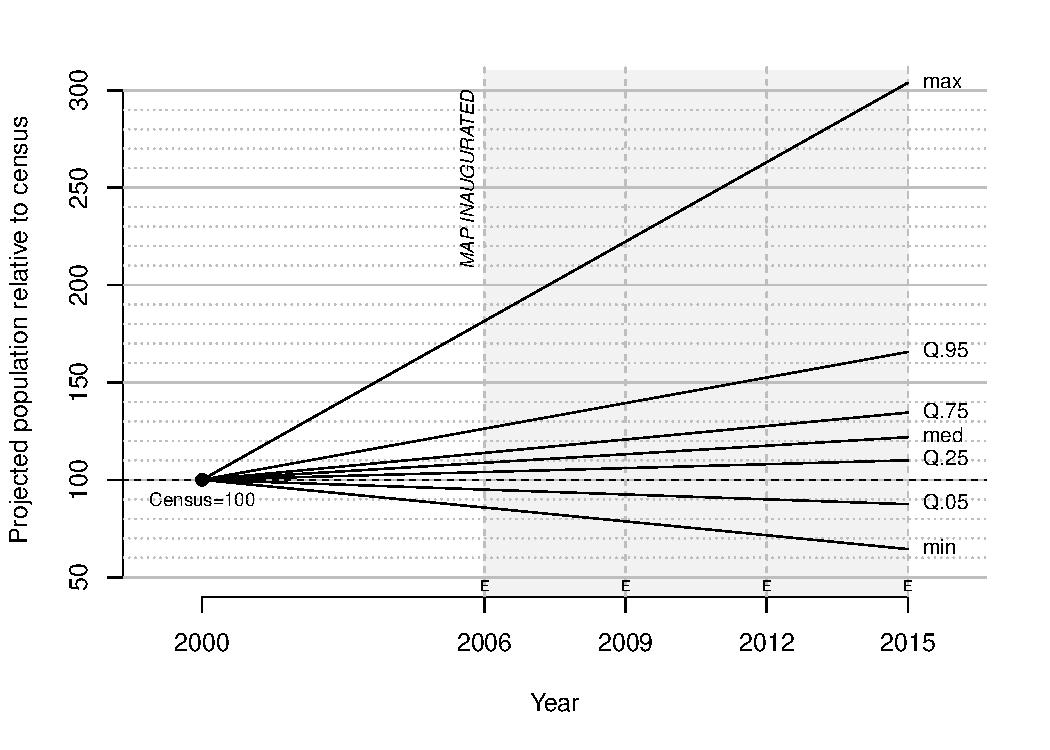
\includegraphics[width=.8\columnwidth]{disRelPopProj2006map.pdf} 
  \caption{The 2006 map and demographic change. Plotted population projections relied on the 2000--2010 censuses rate of change (see text for details). Letters \textsc{e} in the horizontal axis indicate elections using this map. Source: prepared with data from \url{www.inegi.org.mx} and \url{www.ine.mx}.}\label{F:disRelPop2006map}
\end{figure}

Figure \ref{F:disRelPop2006map} illustrates the projection exercise, and how it puts creeping malapportionment within reach to assess its impact on representation. If every district had experienced the same rate of population change, the redistricting census lag would be inconsequential. With variable rates of population growth, malapportionment creeps in. Compared to the 2000 census, projected district populations in 2006, when the map was inaugurated, are off by 9.7\% in absolute value on average, with a standard deviation of 10.6\%. Indexing 2000 census district populations at 100, as the figure does, reveals how different the most demographically dynamic units were on paper and in reality. The fastest-growing district was 88\% larger in 2006 than what census data otherwise suggested (the line labeled `max'). The district shedding most population was 16\% smaller (the `min' line). These are outliers, but central tendencies reflect sizable lags as well. The inter-quartile range (lines Q.25 and Q.75) covered 1\%--13\% above census in the 2006 election, and expanded to 4\%--20\%, 7\%--27\%, and 10\%--35\% in the three subsequent Diputado elections using the same map.

Estimating intercensal populations non-linearly is also preferable to our linear approach. The key problem on this front appears to be the choice of a functional form that both smoothes the inter-census rate of population growth while also taking the values actually observed on three census years (2000, 2005, and 2010). An exponential form between pairs of census counts \citep{dasGupta1978RateGrowth} does a good job for years between observations, but not before and after, nor does it treat transitions from one pair to the next smoothly. A polinomial form would allow work with all three census counts, but also seems problematic for proecting estimates beyond 2010. We therefore abandoned the attempt to refine population estimates non-linearly.

\subsection*{Step 3: Simulate national-level elections}

In order to simulate national elections (i.e., a vote-seat share for each party), the Linzer method infers the distribution of district-level returns from every pair of parties' correlations. Some parties do not field candidates in every district, so finding district patterns of party contestation starts the process \citep[][:405]{linzerSeatVoteElasticity2012}. For example, two patterns were observed in 2009: the PAN, PRI, PRD, and MC contested 63 districts, while the same plus the Green party contested the remainder 237 districts. Subsets of districts in each pattern are analyzed separately. To also take district population and turnout into account, the patterns of contestation also include the abstention rate, as discussed in step 1. 

% plot prepared in linzerElas.r
\begin{figure}
\centering 
  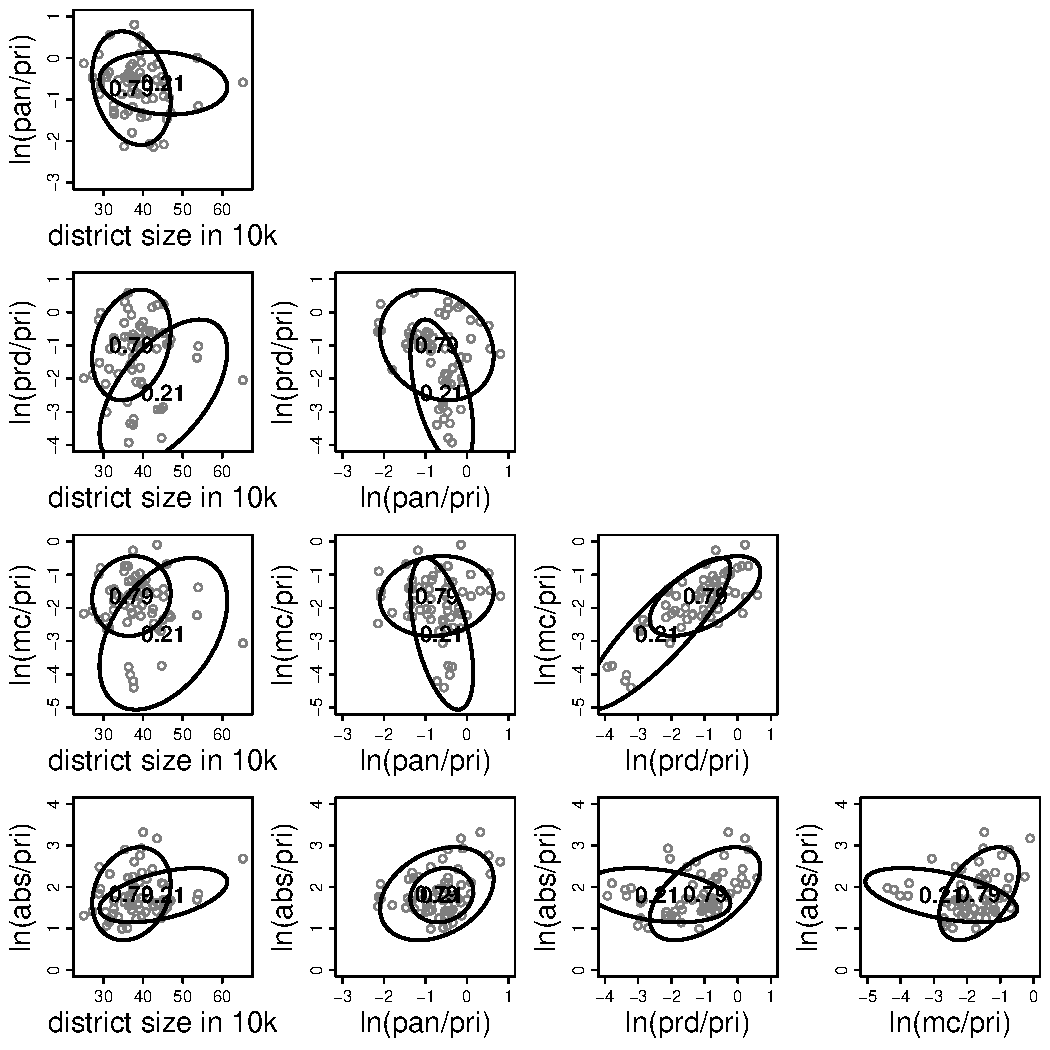
\includegraphics[width=.8\columnwidth]{linzerCorrelat2009.pdf} 
  \caption{How pairs of parties' votes correlated (vis-\`a-vis the PRI) in 2009: 63 districts that the Green party did not contest}\label{F:linzerCorr}
\end{figure}

The density of district returns is unlikely to conform to a textbook statistical distribution. But a mix (superimposition) of multi-variate normals will capture much of the observed variance. Exploration of district outcomes by plotting the relative performance of party pairs (including abstention) relative to the PRI in 2009 (first pattern of contestation) reveals two apparent clusters of districts. In one, including 21 percent of districts in the pattern, MC won/lost votes relative to the PRI ($\ln(\frac{mc}{pri})$ increases) without hurting PAN's performance relative to the PRI ($\ln(\frac{pan}{pri})$ constant); in the other cluster, accounting for 79 percent of districts, PAN won/lost votes relative to the PRI without much affecting how MC performed relative to the PRI. The same is generally true of the PRD and the PAN (as seen in the $\ln(\frac{prd}{pri})$ and $\ln(\frac{pan}{pri})$ plot), but not of the PRD and MC (districts where one grew relative to the PRI also had the other growing relative to the PRI). Choosing the number of components to use is impressionistic \citep[][:405]{linzerSeatVoteElasticity2012}: we proceeded with a single component for the first pattern of 2003 (hypothetical map), for both patterns of 2015 (status quo map), and for the second pattern of 2015 (hypothetical map); two components for the second pattern of 2003 (hypothetical map), for the first pattern of 2015 (hypothetical map), and for both patterns of 2003 (status quo map), 2009, and 2012; and three components for the sole pattern of 2006.

% plot prepared in linzerElas.r
\begin{figure}
\centering 
  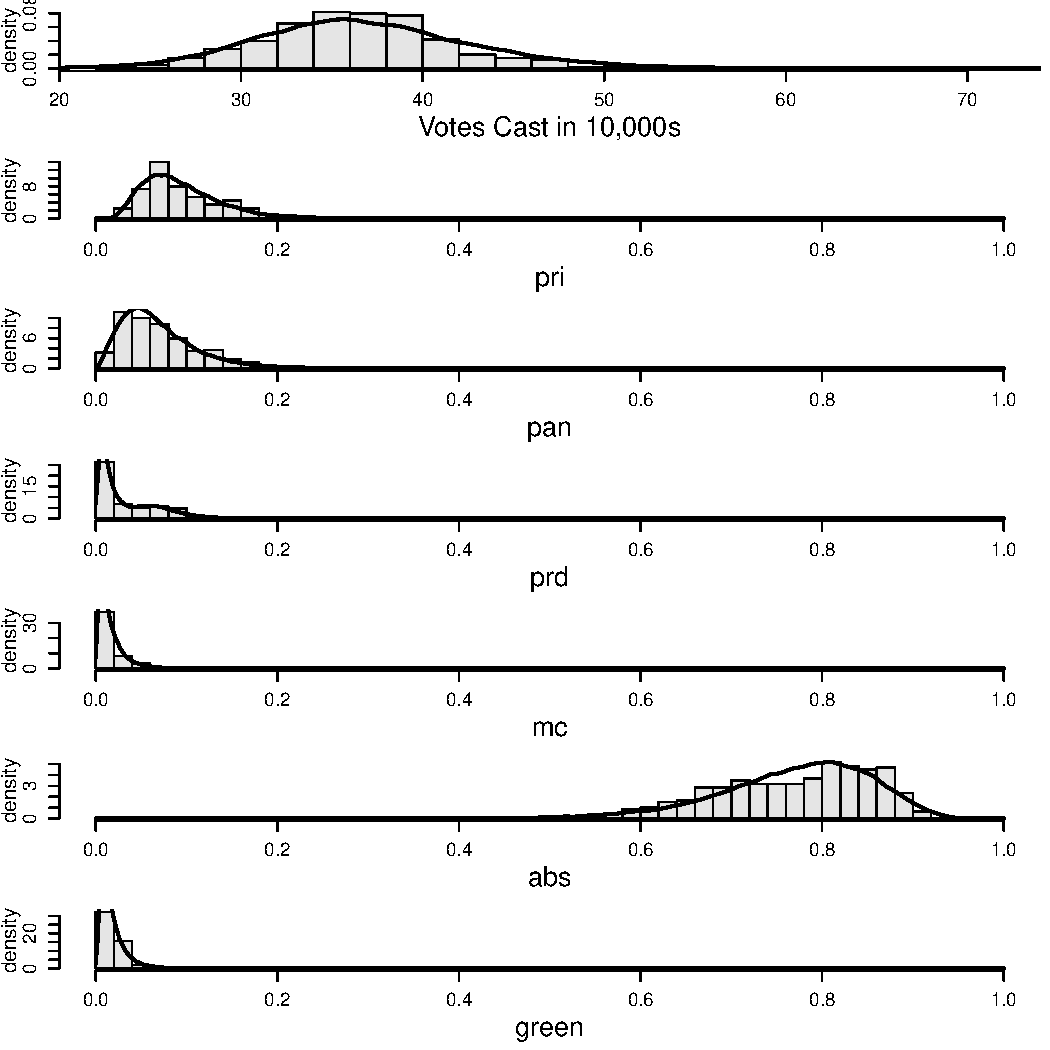
\includegraphics[width=.7\columnwidth]{linzerMg2009.pdf} 
  \caption{Mixture model's marginal densities in 2009}\label{F:linzerMg}
\end{figure}

Figure \ref{F:linzerMg} compares observed 2009 frequencies with the mixture model's marginal density to verify that there is a good match between the two. Other than a slight bimodality in the abstention rate, marginals follow the contour neatly. Monte Carlo sampling with a weighted mix of the bi-variate normals generated one thousand simulated elections for 2009 in the analysis. The procedure is identical for all other years/maps. 

%Original version starts by dropping parties irrelevant for analysis (and possibly none), recomputing vote shares so that those remaining add up to 1. (Effective district votes, equal the vote total minus votes for parties dropped and voided ballots, serve as denominator.) A $D=300 \times P=6$ matrix $v$ ensues (as well as seat shares matrix $s$ of same dimensionality). In our version, we include a $P+1$th column reporting the abstention, equal the total district population minus effective vote. District population serves as denominator to produce vote shares. 

\subsection*{Step 4: Estimate responsiveness and partisan bias}

We use MCMC to estimate equation \ref{E:kingMulti}, implemented with Jags \citep{jags.cite}, called from R \citep{r.cite}. Preparation involves generating data objects first: $i$ indexes $I=100$ simulated observations for a given year; $p$ indexes $P=6$ parties in the analysis; and $D=300$ is the number of plurality districts; votes and seats $I\times P$ matrices $\texttt{v}$ (where $\texttt{v}_{i,p}$ is party $p$'s vote share in the $i$th simulated election) and $\texttt{S}$ (where $\texttt{S}_{i,p}$ are the seats that party $p$ won in the $i$th simulation); and a $P$-length vector $\texttt{dummy}$ (where $\texttt{dummy}_p$ equals 1 if party $p$ contested the election in the given year, 0 otherwise). Our single-year research design avoids the obstacle posed by elections with varying sets and sizes of candidates in in MCMC estimation (an analyst could adapt the Bugs model in Table \ref{T:bugsCode} to the number of parties in the simulated elections). The code, however, is prepared to tackle a multi-year estimation with different contestation patterns: $\texttt{dummy}$ indicates parties contesting each election and fed to the MCMC process. Each additive component of the numerator and denominator (i.e., the party's $\lambda * v^\rho$) is multiplied by the corresponding dummy, so that parties not contesting drop from the likelihood function. All data objects are bundled in a list 

\begin{center}
\lstinline[language=R]!lrdata <- list("S", "v", "I", "J", "D", "dummy")!.
\end{center}

\noindent We next randomize a set of initial values for the model parameters ($\lambda$ needs only $J-1=5$ initial values because we restrict $\lambda_{\text{PRI}}=0$)

\begin{center}
\lstinline[language=R]!lrinits <- function(){ list (lambda=rnorm(J-1), rho=rexp(1)) }!
\end{center}

\noindent and define objects to store  parameters' posterior distribution samples

\begin{center}
\lstinline[language=R]!lrparameters <- c("lambda", "rho")!.
\end{center}

\lstset{style=mystyle}
\begin{table}
\centering
\setstretch{1}
\begin{lstlisting}[language=R]
lambda.rho <- function() {
  for (i in 1:I){   # loop over observations (simulations)
    for (p in 1:P){ # loop over parties (dummy selects who ran)
      S[i,p] ~ dbin(pi[i,p], D[i])  # D is the number of SMD seats
    }
    numerator[i,1] <- dummy[i,1] * exp( lambda[1] ) * v[i,1]^rho
    numerator[i,2] <- dummy[i,2]                    * v[i,2]^rho
    for (p in 3:P){
      numerator[i,p] <- dummy[i,p] * exp( lambda[p-1] ) * v[i,p]^rho
    }
    for (p in 1:P){ # loop over parties
      d1[i,p] <- dummy[i,1] * exp( lambda[1] ) * v[i,1]^rho 
      d2[i,p] <- dummy[i,2]                    * v[i,2]^rho # reference
      d3[i,p] <- dummy[i,3] * exp( lambda[2] ) * v[i,3]^rho 
      d4[i,p] <- dummy[i,4] * exp( lambda[3] ) * v[i,4]^rho 
      d5[i,p] <- dummy[i,5] * exp( lambda[4] ) * v[i,5]^rho 
      d6[i,p] <- dummy[i,6] * exp( lambda[5] ) * v[i,6]^rho 
      denominator[i,p] <- d1[i,p] + d2[i,p] + d3[i,p] 
                        + d4[i,p] + d5[i,p] + d6[i,p]
      pi[i,p] <- numerator[i,p] / denominator[i,p]
    }
  }
  ### priors
  for (q in 1:5){ # P=6 party labels minus reference party is 5
    lambda[q] ~ dnorm( 0, tau.lambda )
  }
  tau.lambda <- pow(.25, -2)
  rho ~ dexp(.75) # has positive range, med about 1, mean 1.25, max 4.5
}
\end{lstlisting}
\setstretch{2}
\caption{Code for Bugs model}\label{T:bugsCode}
\end{table}

The formal model estimated appears in Table \ref{T:bugsCode}. Reliance on $\texttt{dummy}$ is convenient as is allows to proceed with six-party votes and seats matrices regardless of the year selected---otherwise the code would need to be adapted each year for variable parties, which is trivial. Parties not contesting an election (Morena in 2003--12, Green in 2006, MC in 2006 and 2012), with zero votes and seats columns, need not be dropped from matrices. Instead, multiplying the corresponding $\lambda * v^\rho$ term by contestation $\texttt{dummy}$ annuls them from equation \ref{E:kingMulti}. 

Our multinomial logistic regression type model satisfies the independence of irrelevant alternatives assumption in the same way that King does. Quoting at length: 
\begin{quotation} 
\singlespacing
\noindent [T]he implied assumption of independence of irrelevant alternatives is satisfied ... since the entire stochastic component is conditional on all parties and votes. The only random choice being made is by the electoral system in assigning seats to parties. Therefore, I use the multinomial probability distribution for the number of seats allocated to the $J$ political parties, a straightforward generalization of the binomial \citep[][:168]{king.1990elRespBiasMultiparty}.
\end{quotation} 
The only difference is our use of $P$ seat-allocating binomial distributions instead of one multinomial (line 4 of the code in Table \ref{T:bugsCode}).

R package $\texttt{r2jags}$ \citep{r.r2jags} is a suite of functions to bind all these objects into a Jags call for estimation (and do post-estimation evaluations):

\setstretch{1}
\begin{center}
\begin{tabular}{ll}
\\
results~~<$-$~~\textbf{jags} ( & data = lrdata, \\ 
                  & inits = lrinits, \\
                  & parameters.to.save = lrparameters, \\
                  & model.file = lambda.rho, \\
                  & n.chains = 3, \\
                  & n.iter = 50000, \\
                  & n.burnin = 25000, \\
                  & n.thin = 50~~~). \\ \\
\end{tabular}
\end{center}
\setstretch{2}

\noindent We stop the algorithm after 50 thousand iterations. The first 25 thousand are discarded to let the model adapt by updating the prior distributions of parameters to the data. Non-informative priors were used across the board: $\lambda_q \sim \mathcal{N}(0, 4),~q=1,\ldots5)$ and $\rho \sim \texttt{exp}(\frac{3}{4})$ (the exponential distribution has positive range and, with this parameterization, a median of about 1, a mean of 1.25, and a maximum value of 4.5). Every fiftieth iteration of the final 25 thousand was saved as sample of parameters' posterior distributions (of size $3~\text{chains} \times 25000/50 = 1500$). 

To verify convergence, Tables \ref{T:traceplotStart}--\ref{T:traceplotEnd} plot iterations of the Gibbs sampler (x-axis) and sampled values of model parameters (y-axis). One election/map is reported per Table, and one parameter per plot, with columns selecting three ways to measure votes: raw vote shares ($\texttt{v}$), mean district vote shares ($\bar{\texttt{v}}$), and population-weighted mean district votes ($\bar{\texttt{v}}$). With three chains utilized in each Jags call, plots allow verification of two things: that chains had reached a steady state; and that all chains (one in green, one in red, one in blue in the plots) had converged. With no exception, the parameter samples we report in the text had all converged.

\begin{table}
\centering
\begin{tabular}{cccc}
                     & $\texttt{v}$ & $\bar{\texttt{v}}$ & $\bar{\texttt{w}}$ \\ 
    Dev.             & 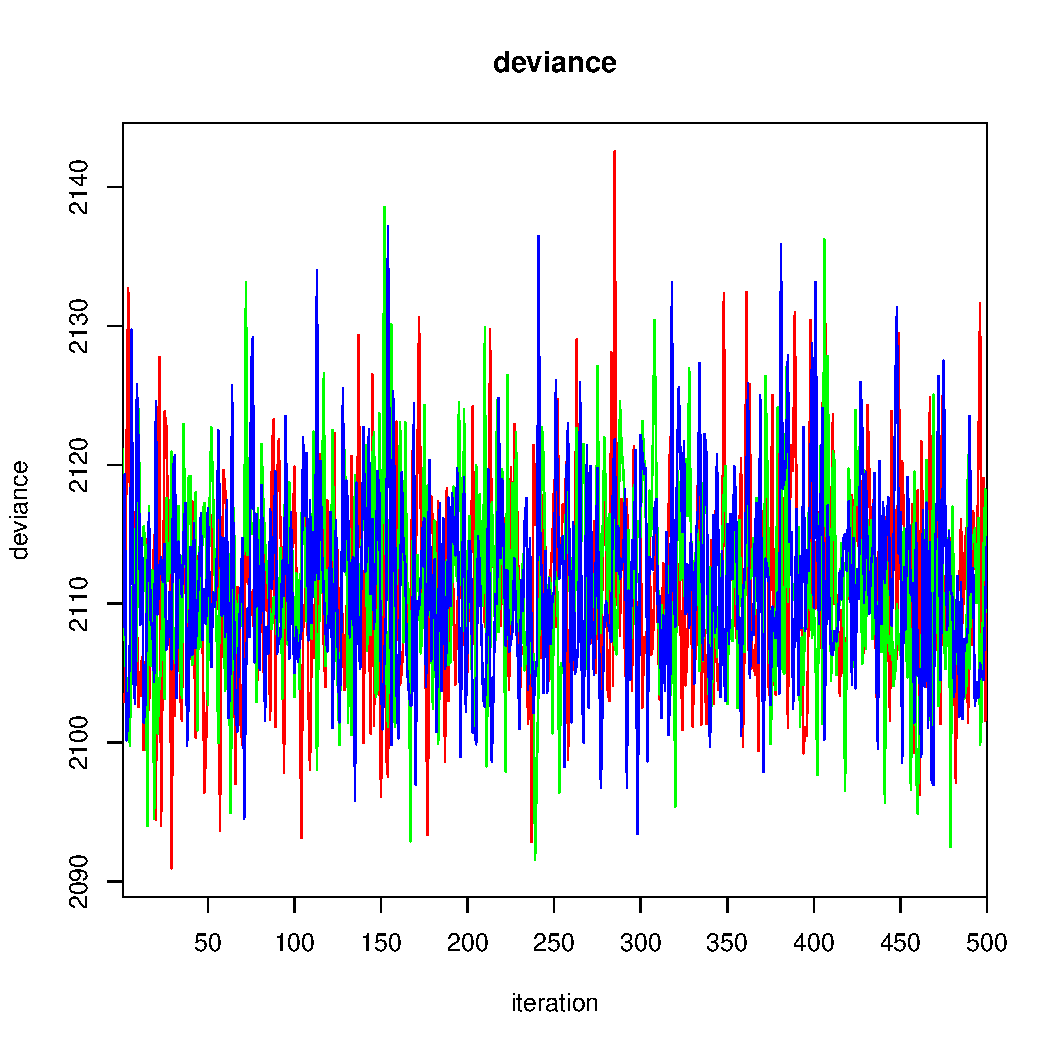
\includegraphics[width=.15\columnwidth]{../graphs/traceplots/2003d97v_1.pdf} &
                        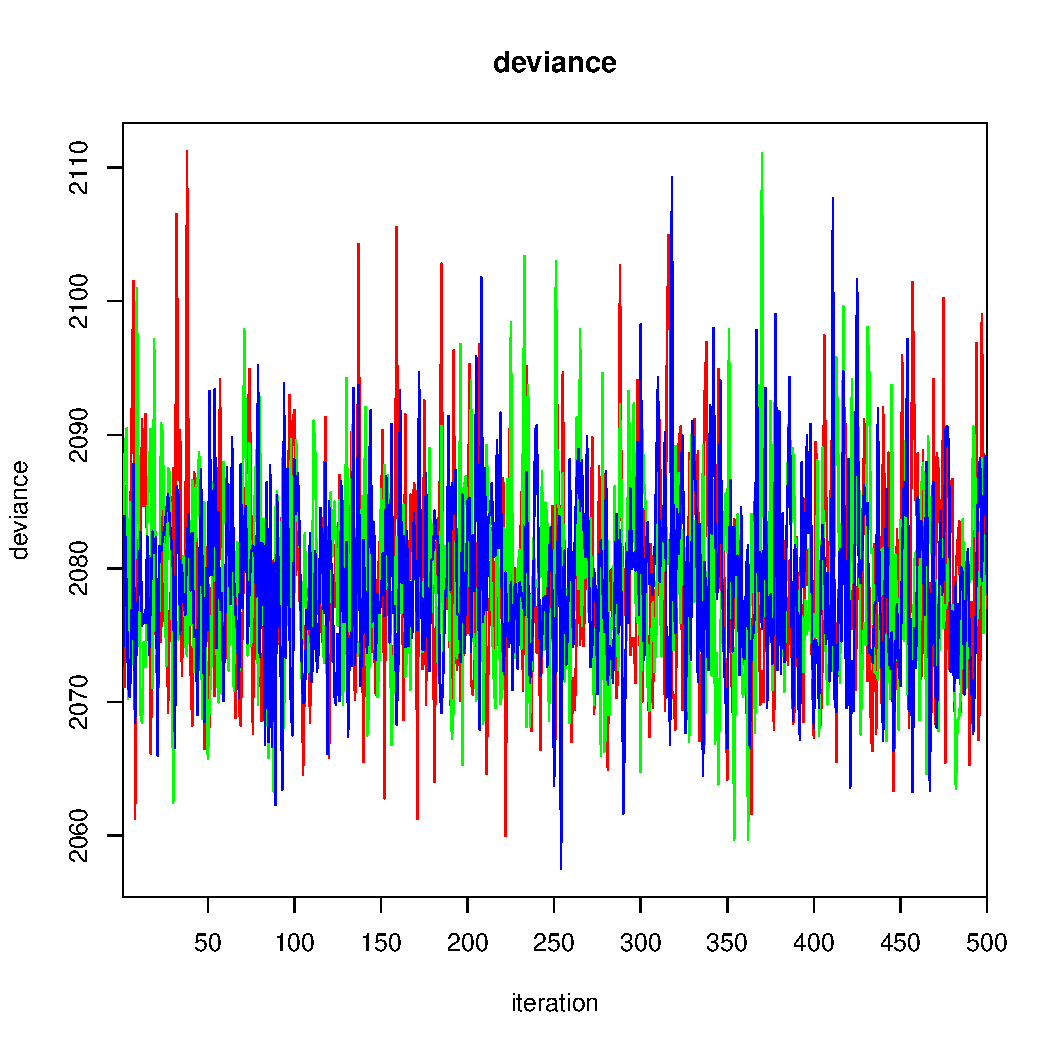
\includegraphics[width=.15\columnwidth]{../graphs/traceplots/2003d97vbar_1.pdf} &
                         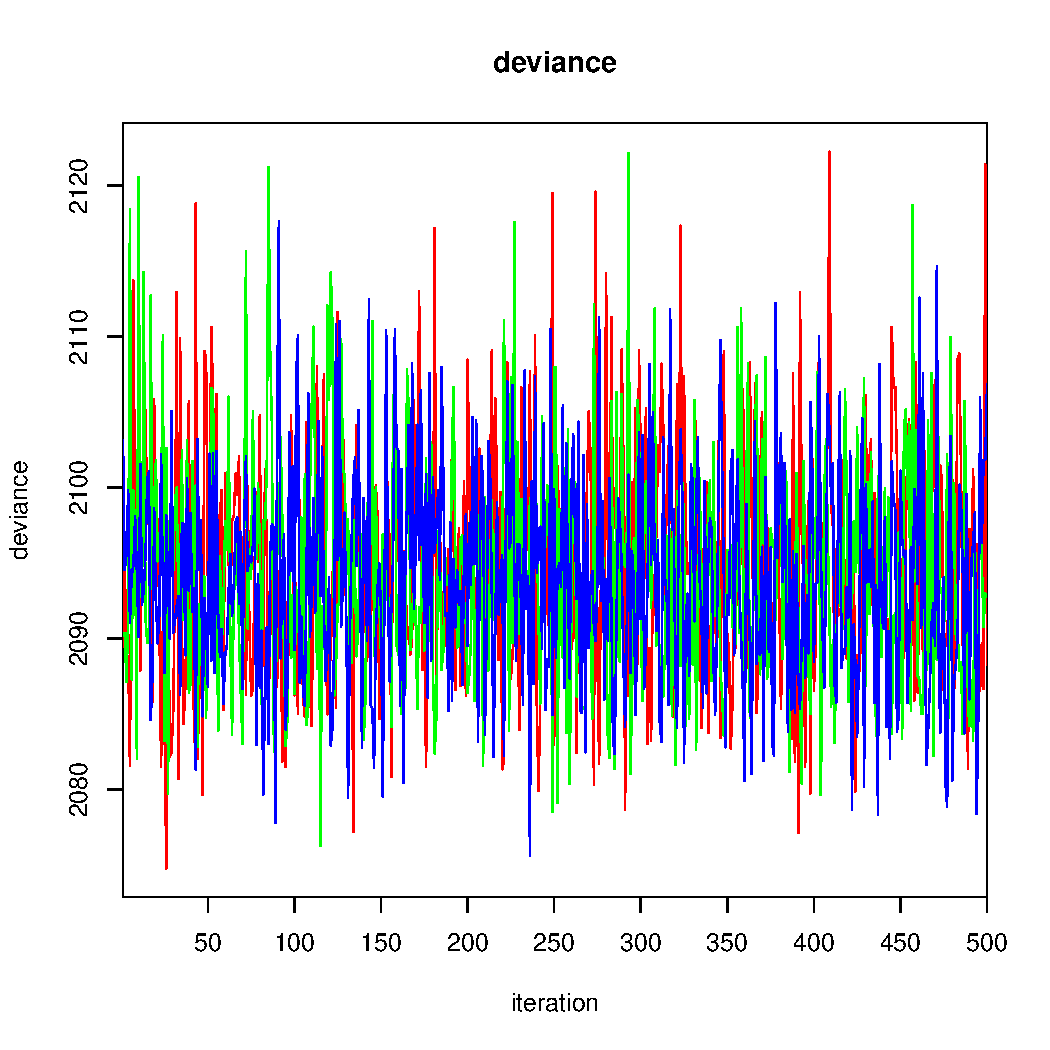
\includegraphics[width=.15\columnwidth]{../graphs/traceplots/2003d97wbar_1.pdf} \\
    $\lambda_{PAN}$   & 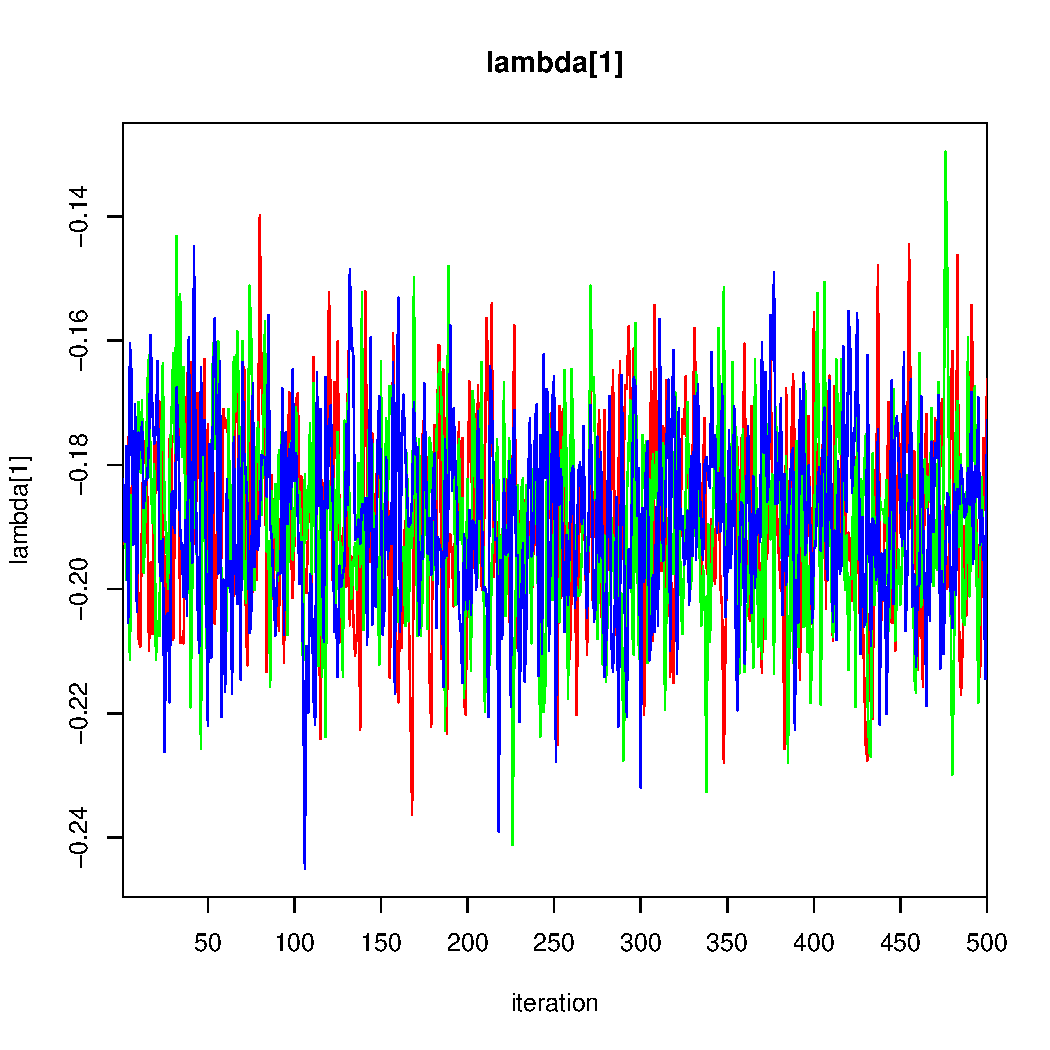
\includegraphics[width=.15\columnwidth]{../graphs/traceplots/2003d97v_2.pdf} &
                        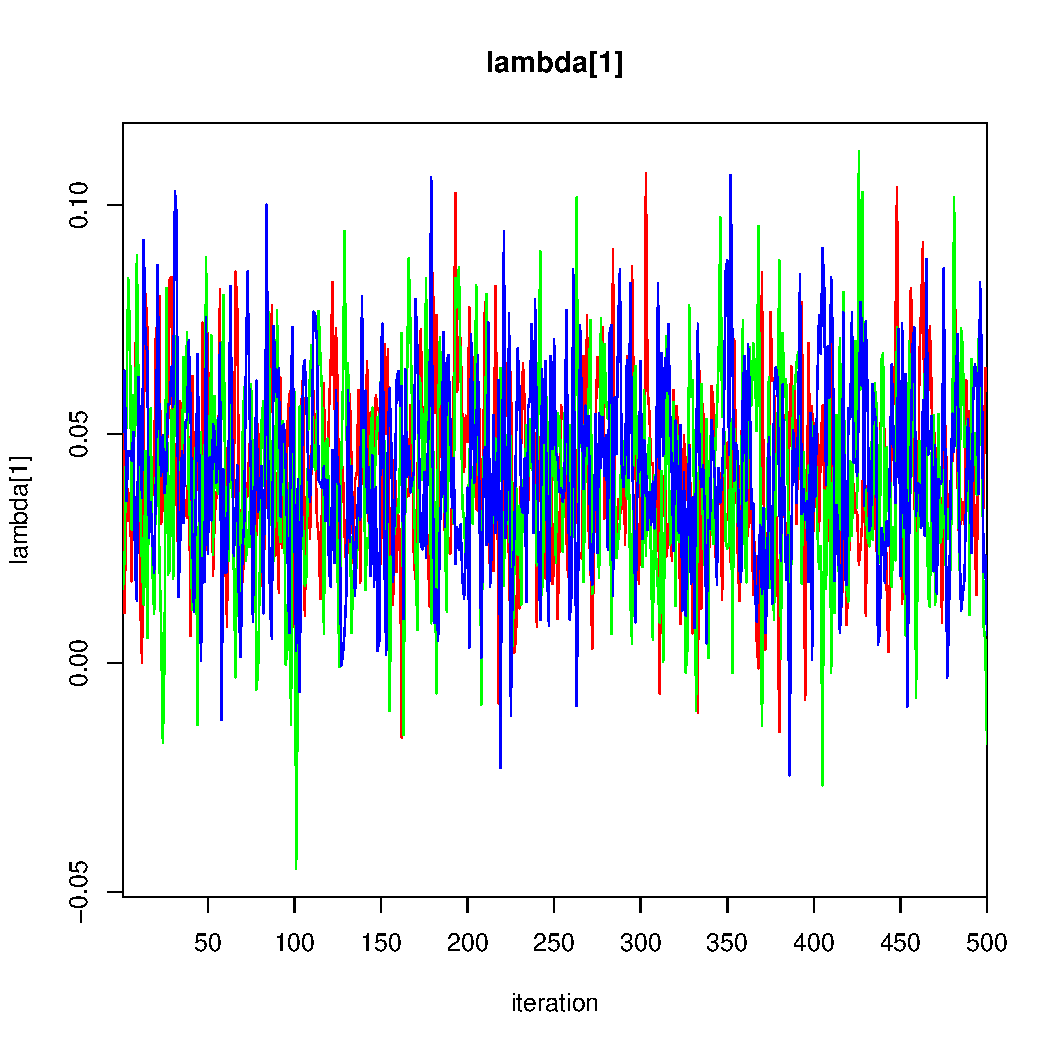
\includegraphics[width=.15\columnwidth]{../graphs/traceplots/2003d97vbar_2.pdf} &
                         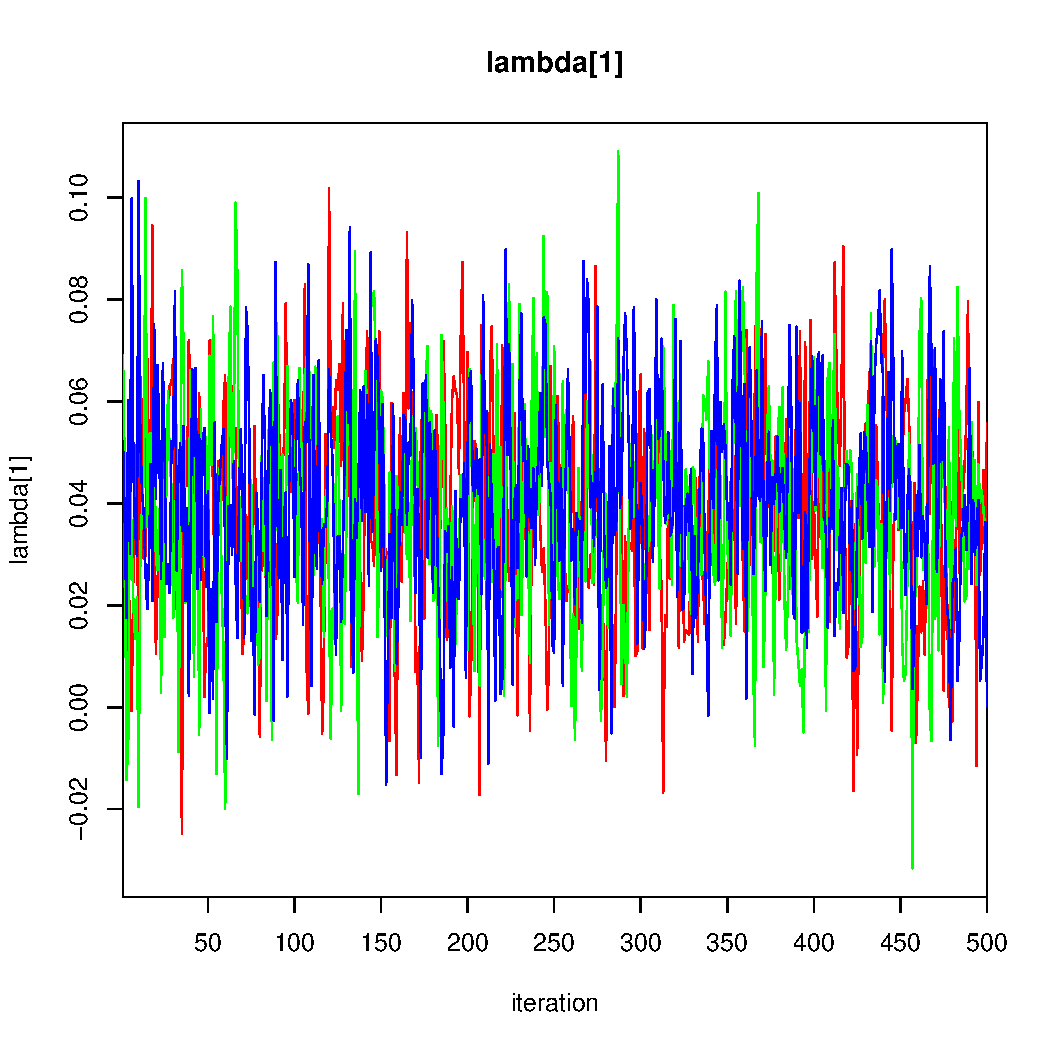
\includegraphics[width=.15\columnwidth]{../graphs/traceplots/2003d97wbar_2.pdf} \\
    $\lambda_{PRD}$   & 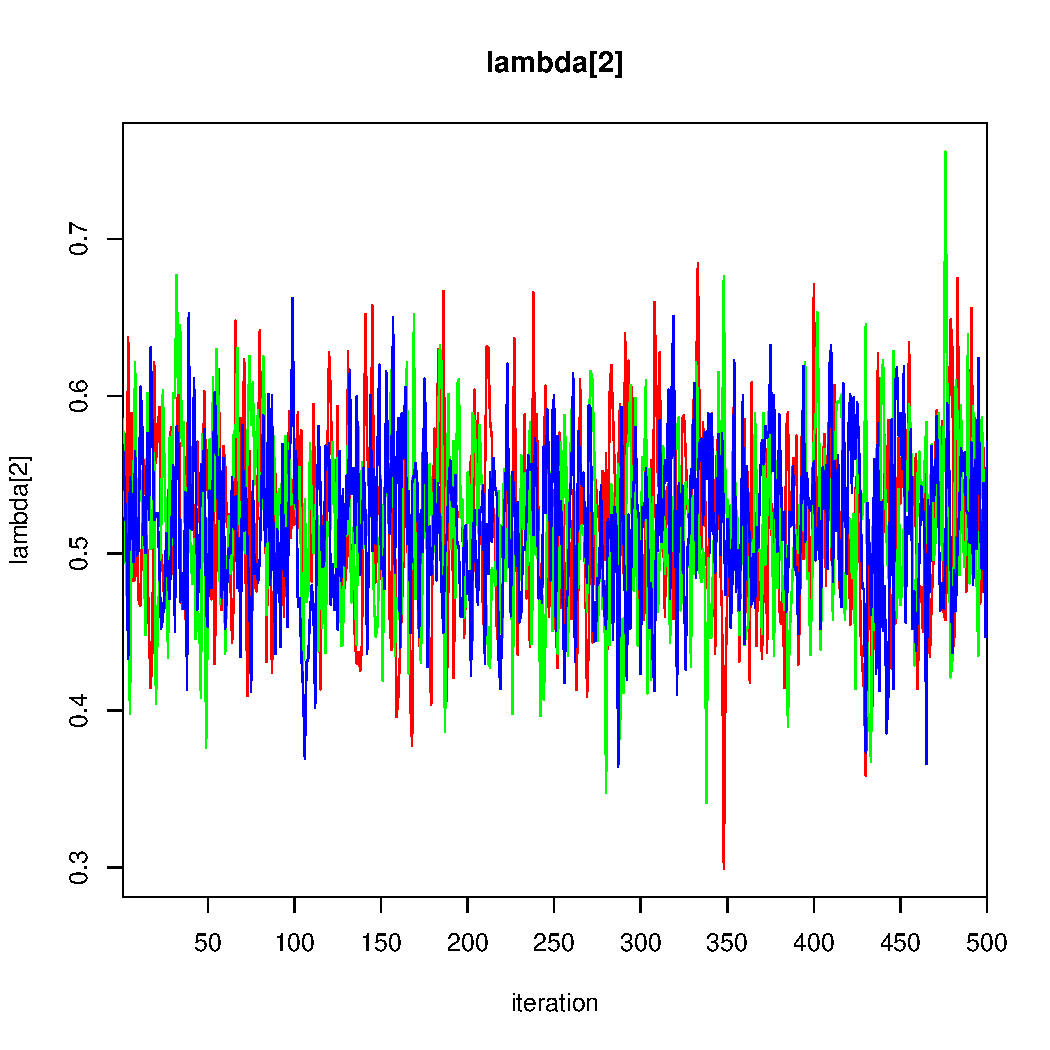
\includegraphics[width=.15\columnwidth]{../graphs/traceplots/2003d97v_3.pdf} &
                        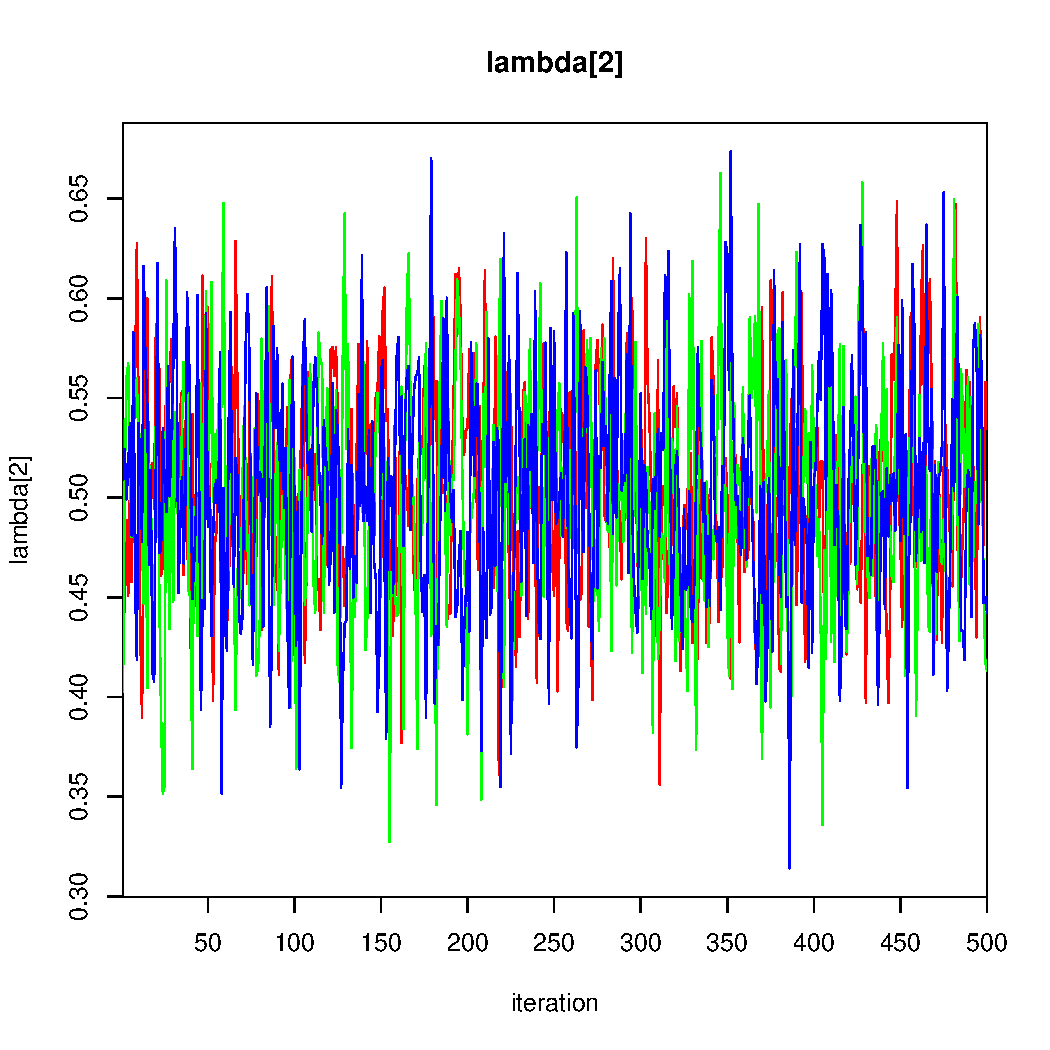
\includegraphics[width=.15\columnwidth]{../graphs/traceplots/2003d97vbar_3.pdf} &
                         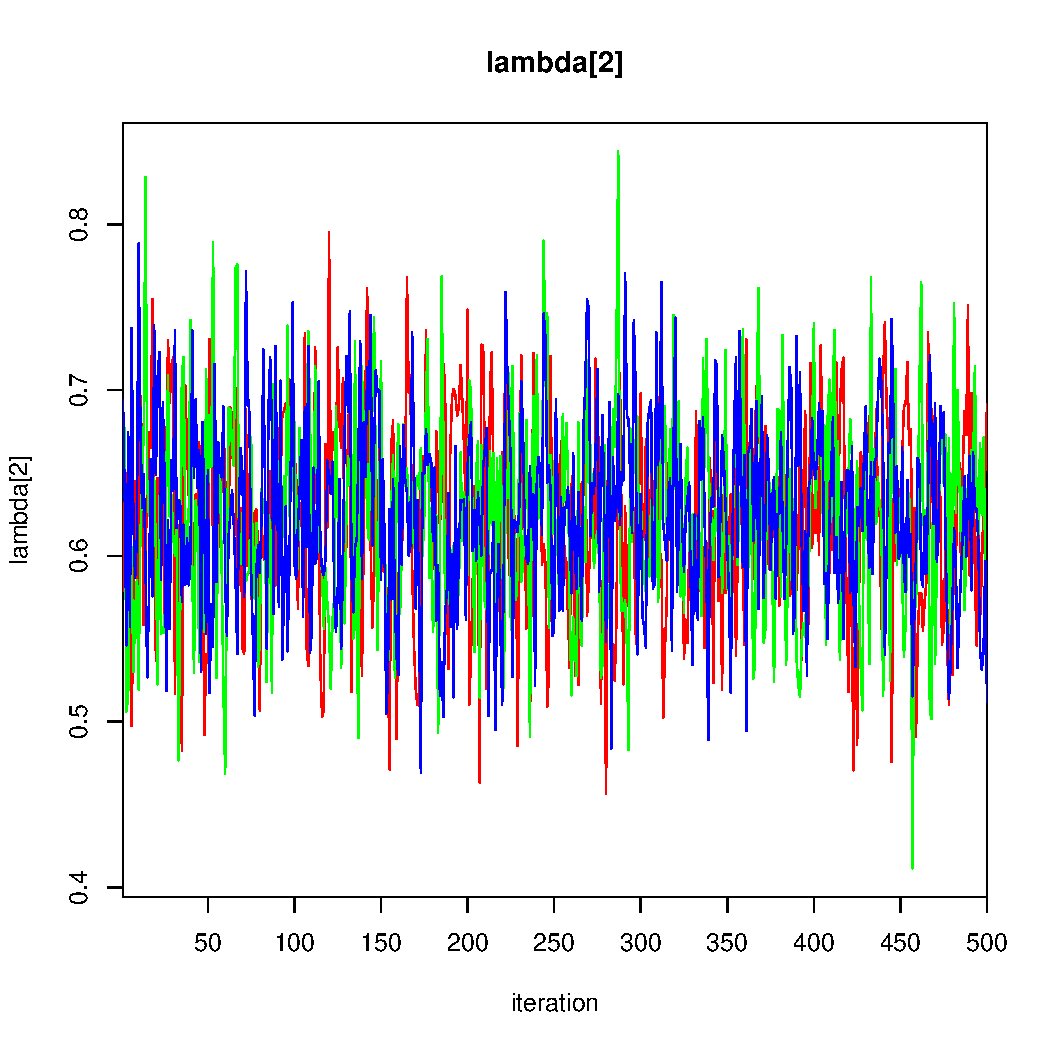
\includegraphics[width=.15\columnwidth]{../graphs/traceplots/2003d97wbar_3.pdf} \\
    $\lambda_{Green}$  & 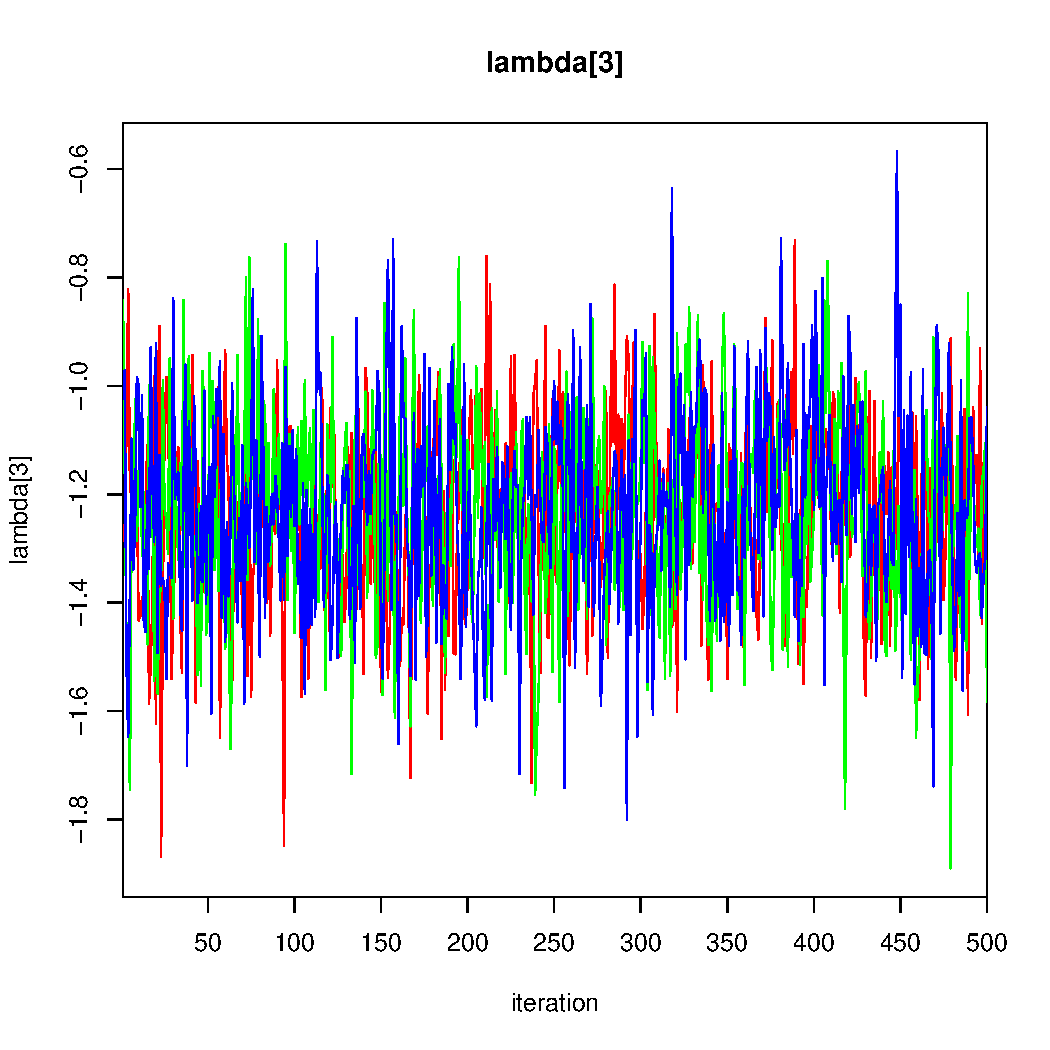
\includegraphics[width=.15\columnwidth]{../graphs/traceplots/2003d97v_4.pdf} &
                        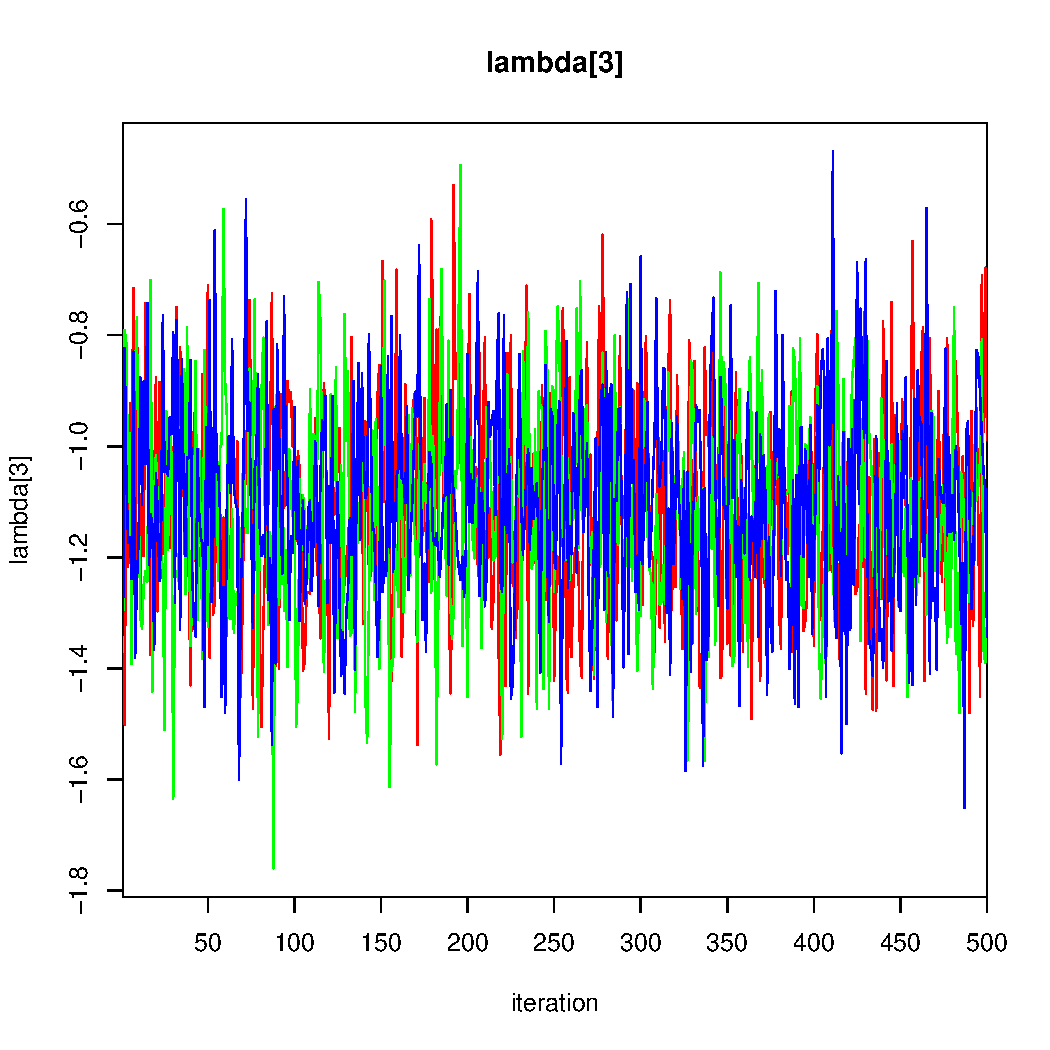
\includegraphics[width=.15\columnwidth]{../graphs/traceplots/2003d97vbar_4.pdf} &
                         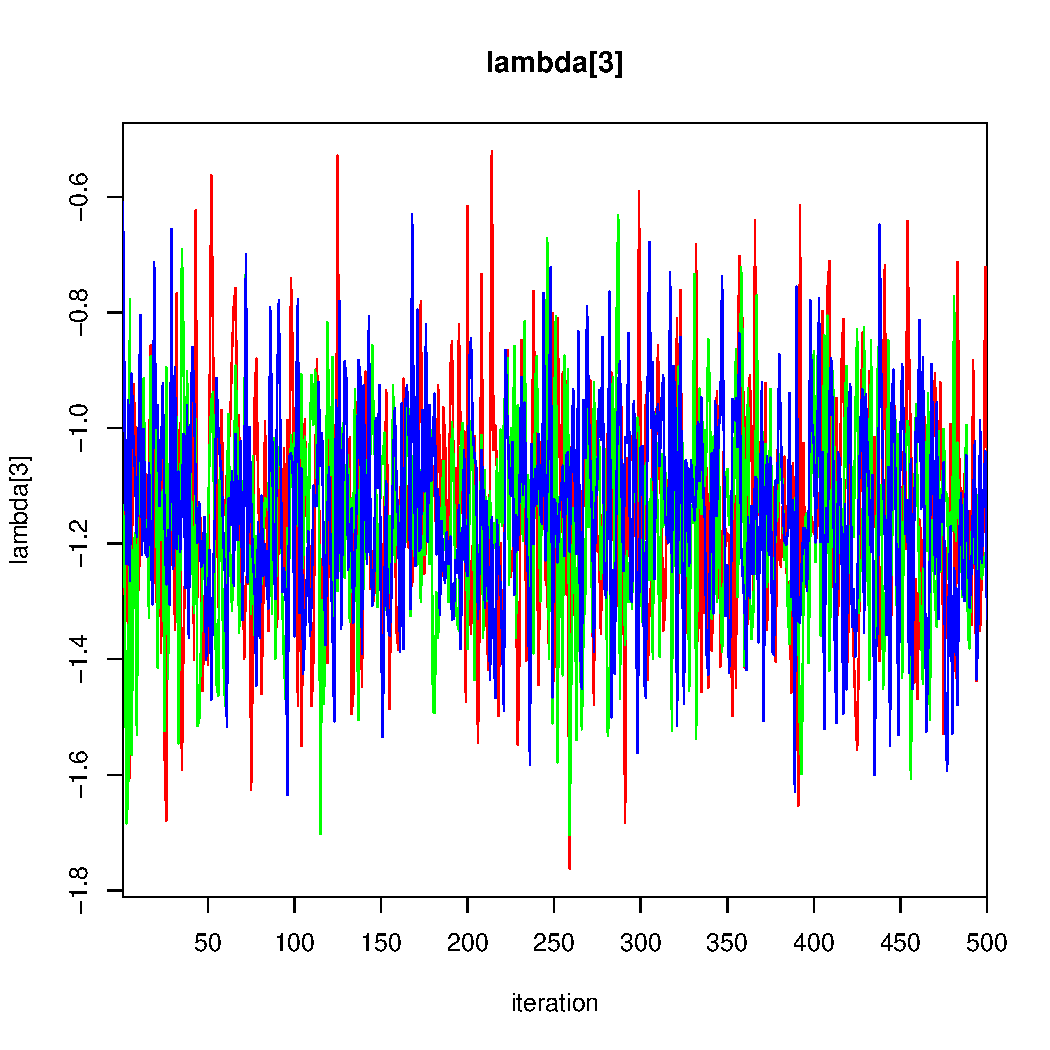
\includegraphics[width=.15\columnwidth]{../graphs/traceplots/2003d97wbar_4.pdf} \\
    $\lambda_{MC}$    & 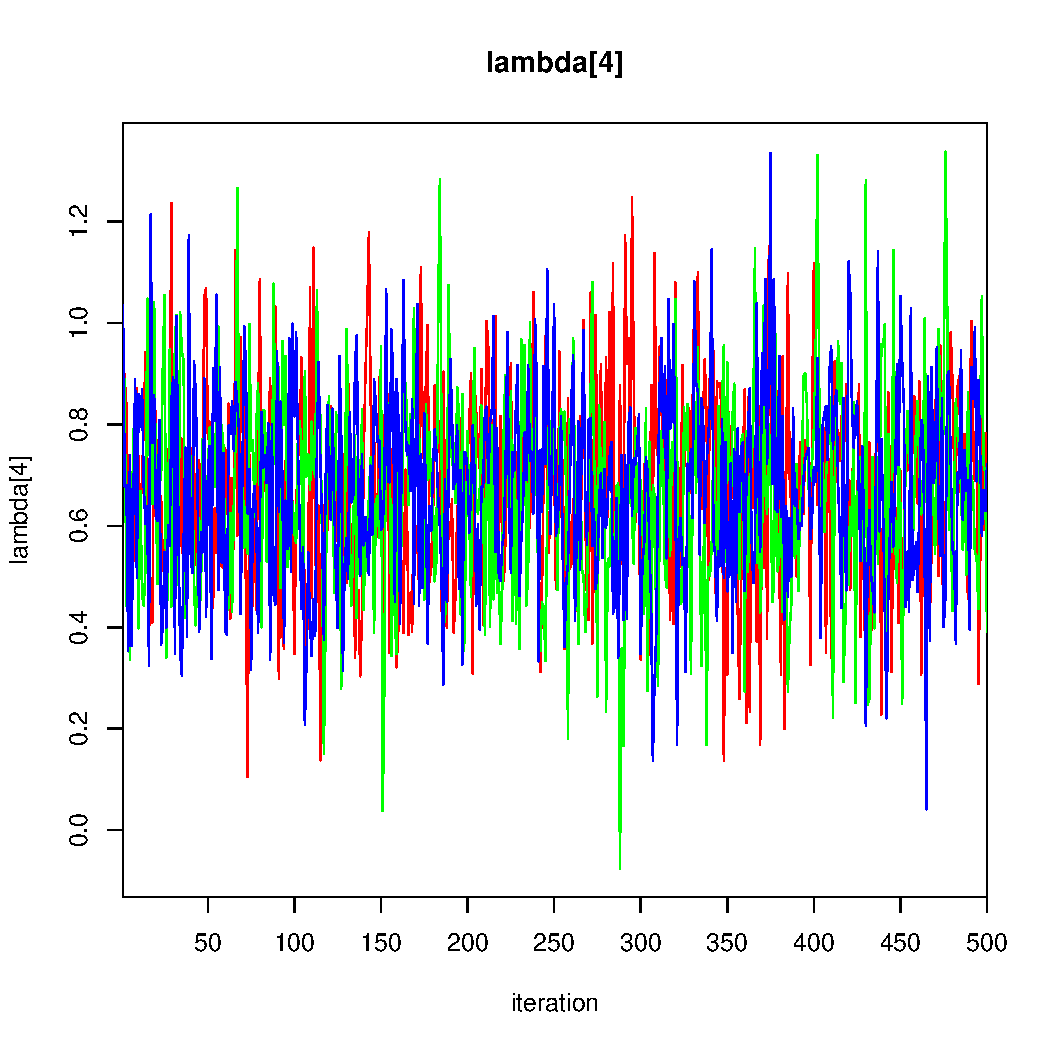
\includegraphics[width=.15\columnwidth]{../graphs/traceplots/2003d97v_5.pdf} &
                        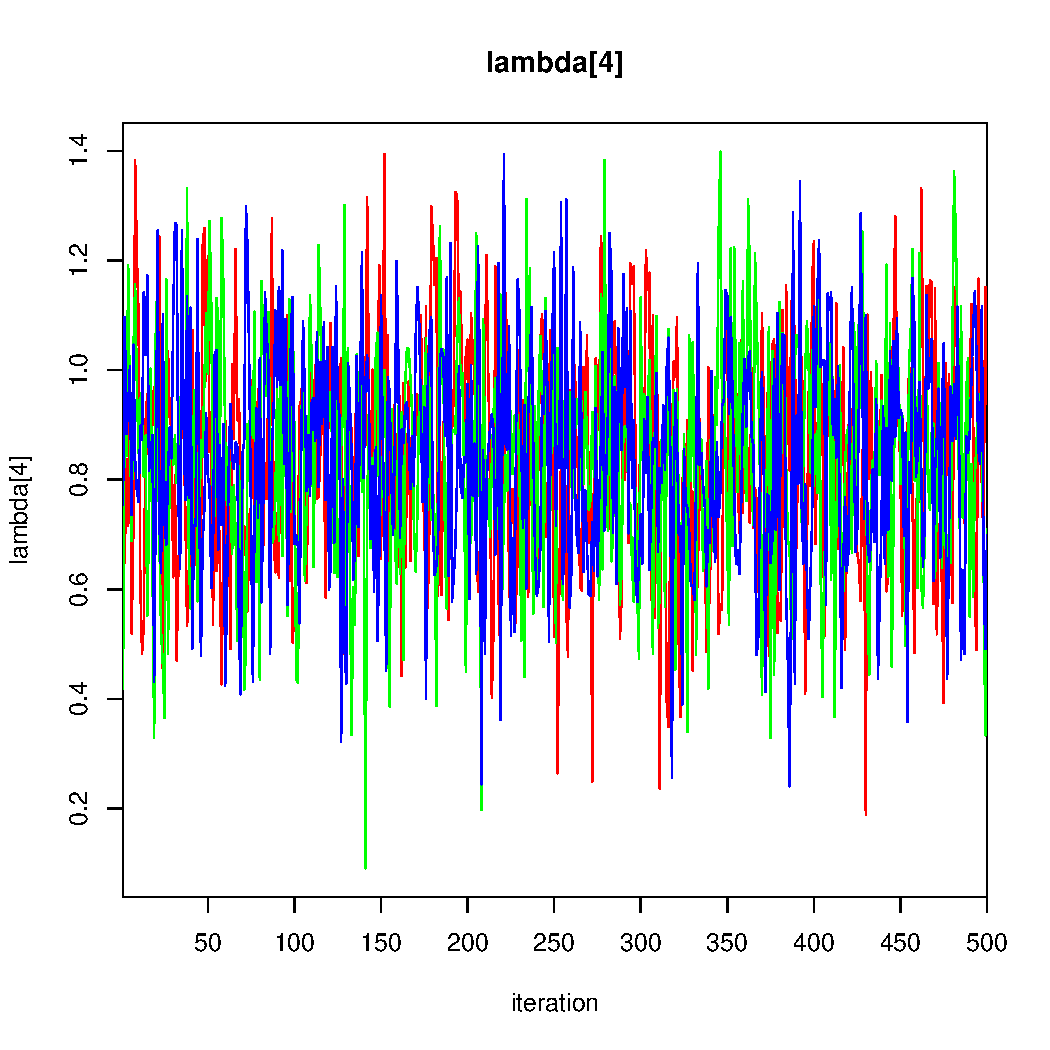
\includegraphics[width=.15\columnwidth]{../graphs/traceplots/2003d97vbar_5.pdf} &
                         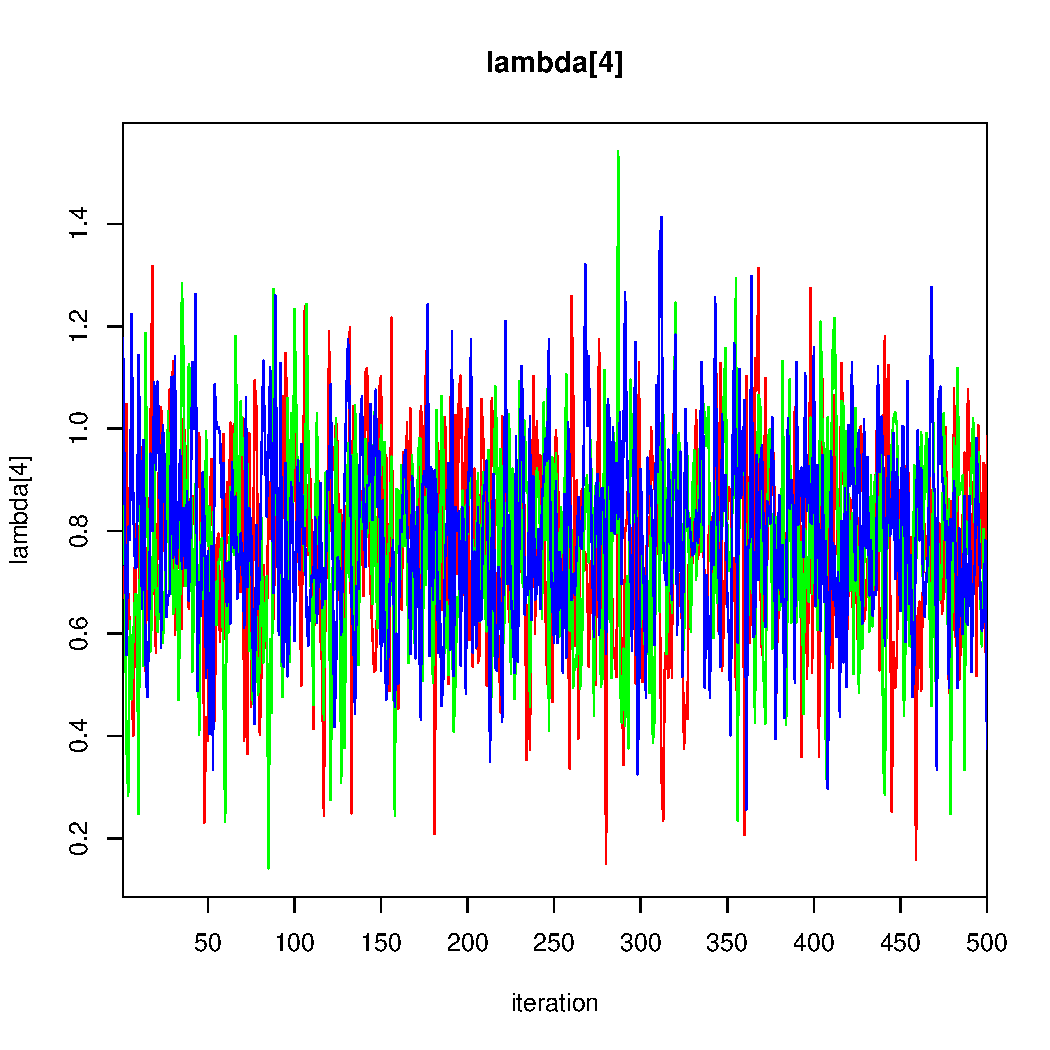
\includegraphics[width=.15\columnwidth]{../graphs/traceplots/2003d97wbar_5.pdf} \\
    % $\lambda_{morena}$ & 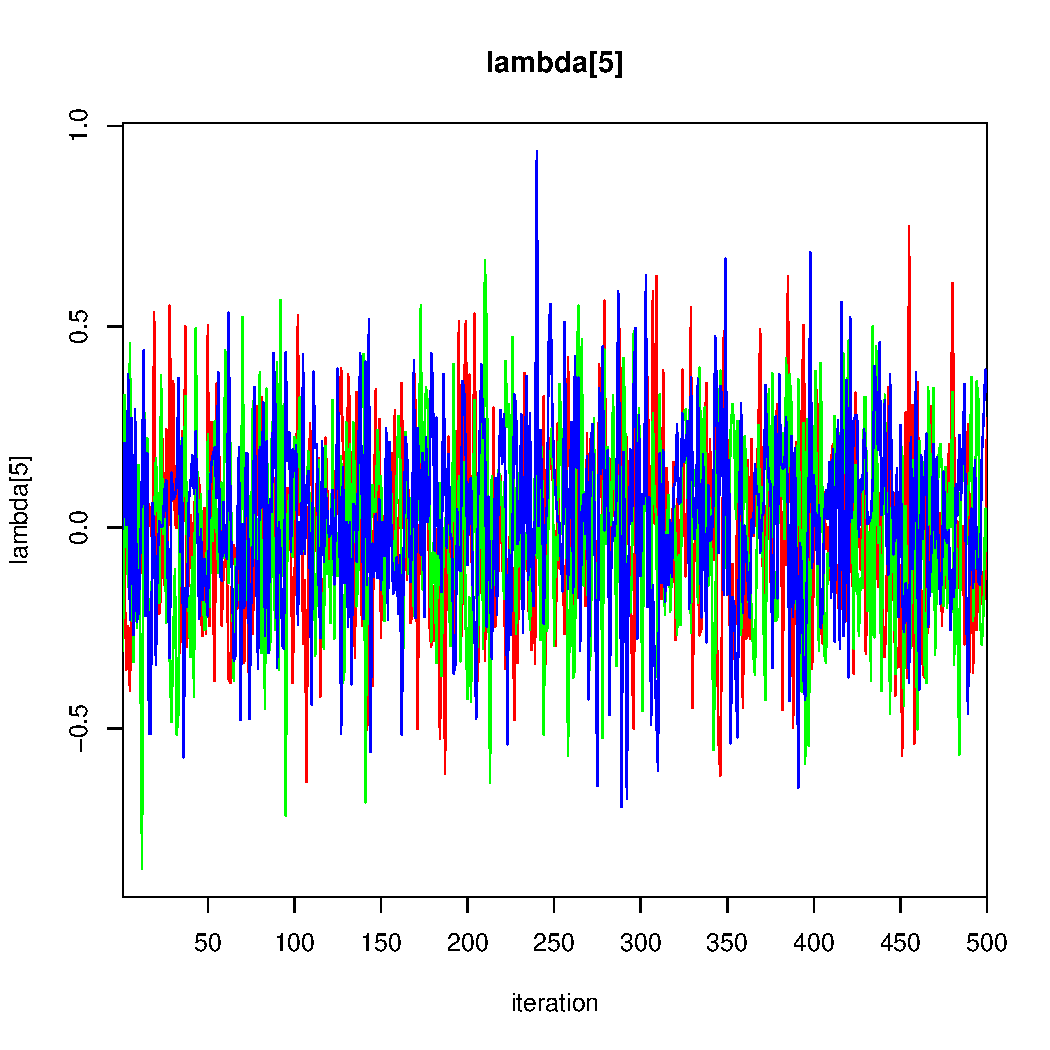
\includegraphics[width=.15\columnwidth]{../graphs/traceplots/2003d97v_6.pdf} &
    %                     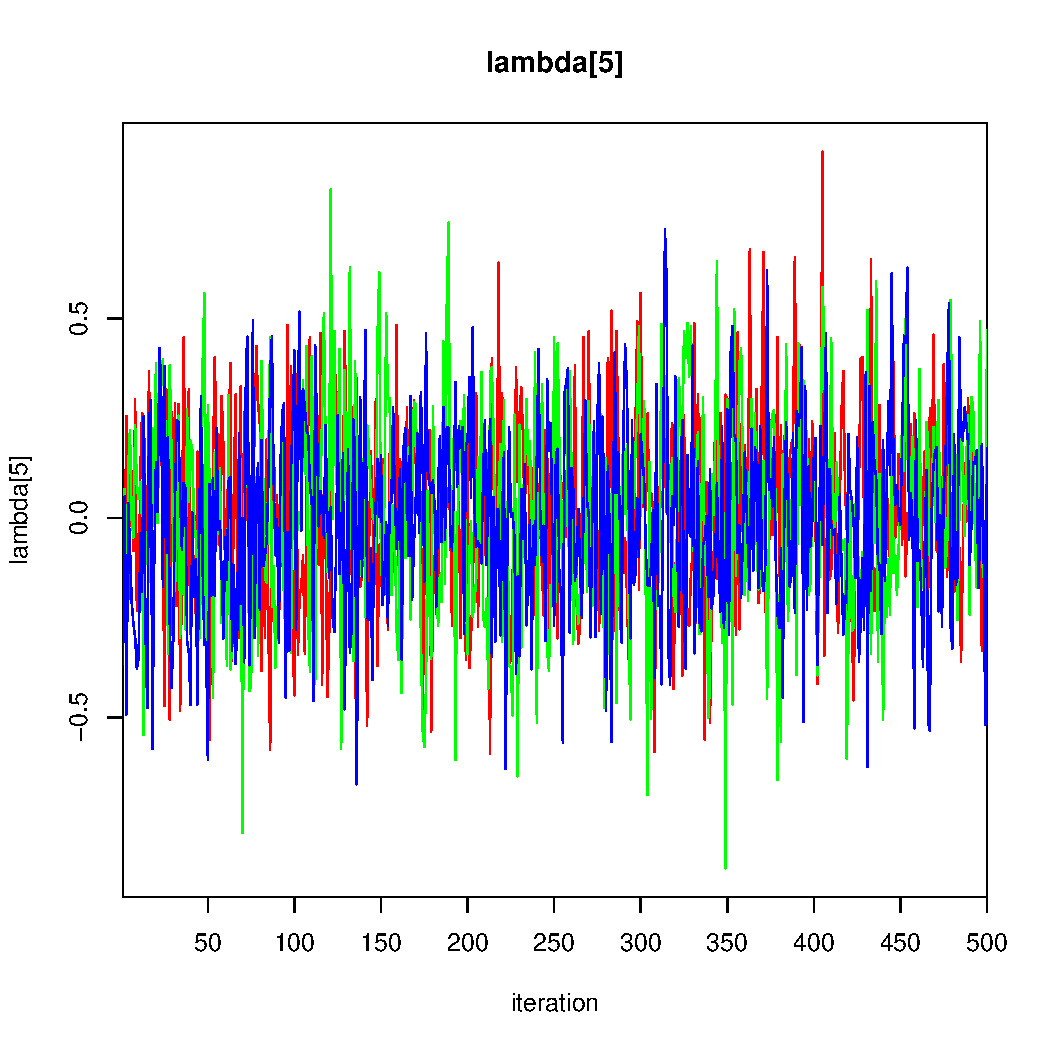
\includegraphics[width=.15\columnwidth]{../graphs/traceplots/2003d97vbar_6.pdf} &
    %                      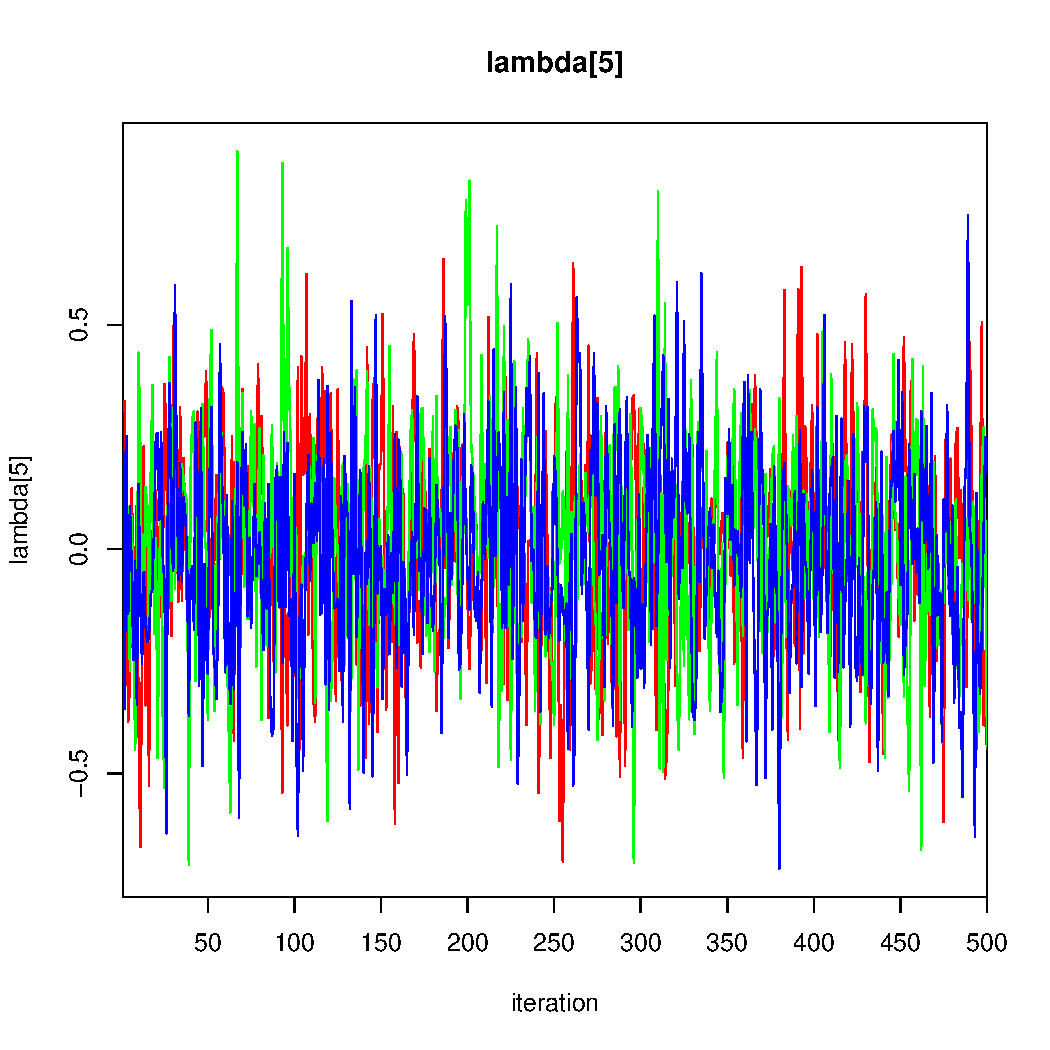
\includegraphics[width=.15\columnwidth]{../graphs/traceplots/2003d97wbar_6.pdf} \\
    $\rho$           & 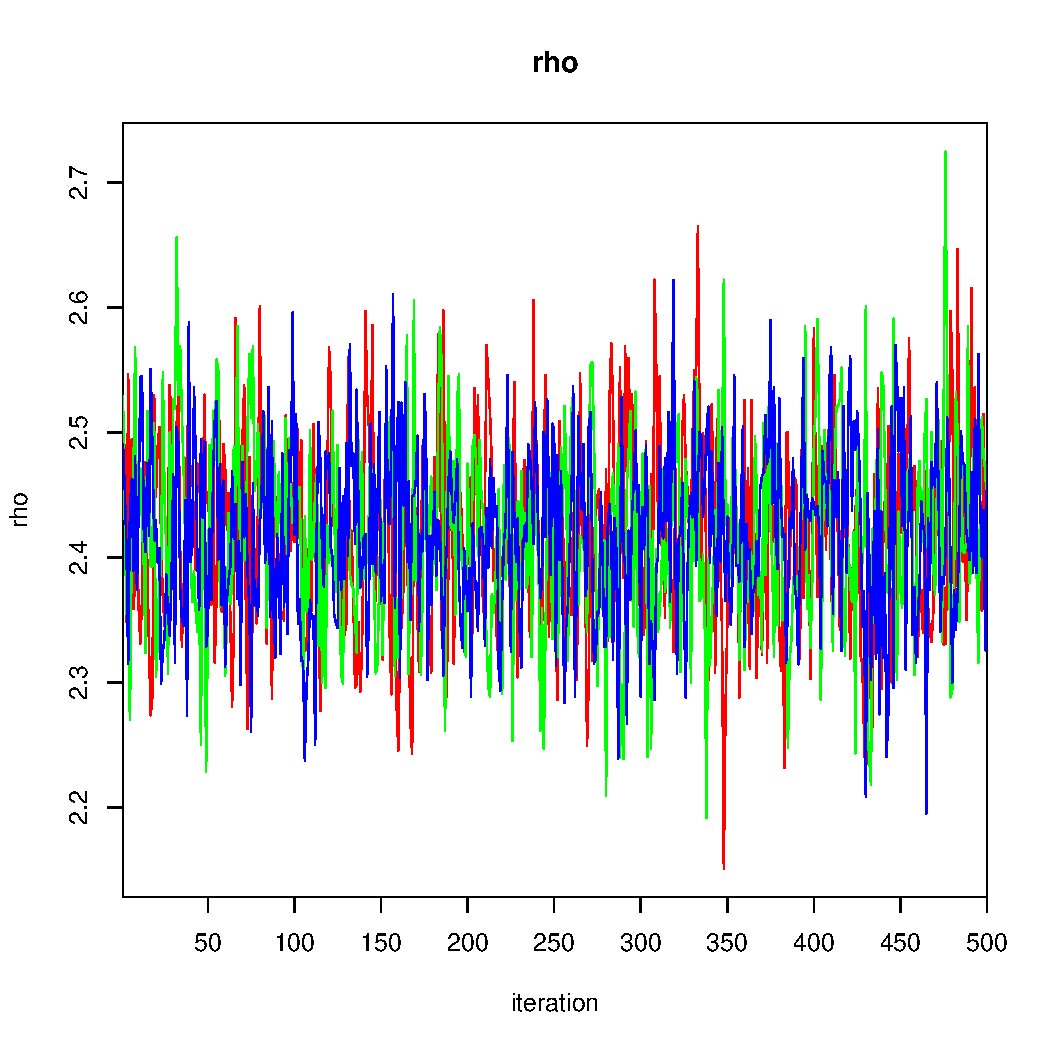
\includegraphics[width=.15\columnwidth]{../graphs/traceplots/2003d97v_7.pdf} &
                        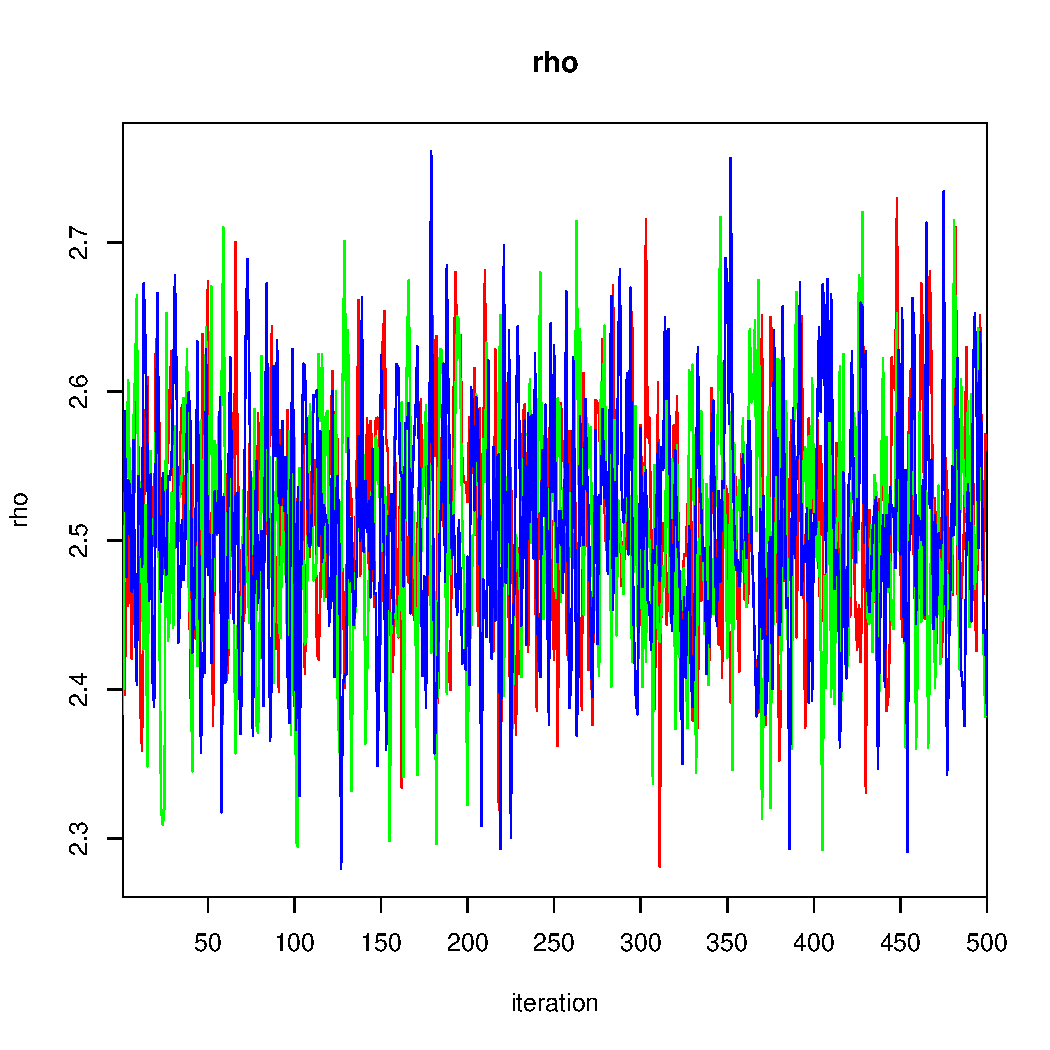
\includegraphics[width=.15\columnwidth]{../graphs/traceplots/2003d97vbar_7.pdf} &
                         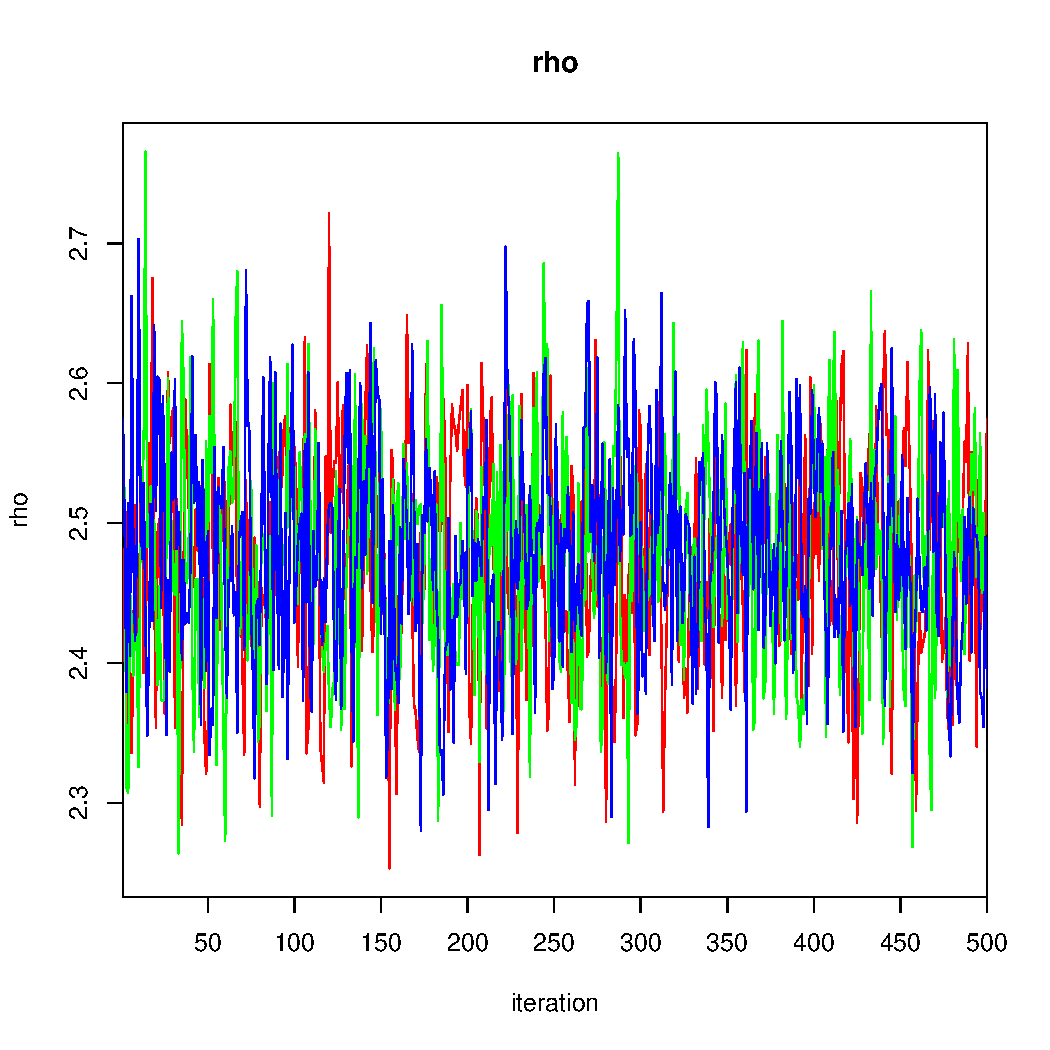
\includegraphics[width=.15\columnwidth]{../graphs/traceplots/2003d97wbar_7.pdf} \\
\end{tabular}
\caption{Three-chain traceplots for 2003 with status quo map}\label{T:traceplotStart}
\end{table}

\begin{table}
\centering
\begin{tabular}{cccc}
                     & $\texttt{v}$ & $\bar{\texttt{v}}$ & $\bar{\texttt{w}}$ \\ 
    Dev.             & 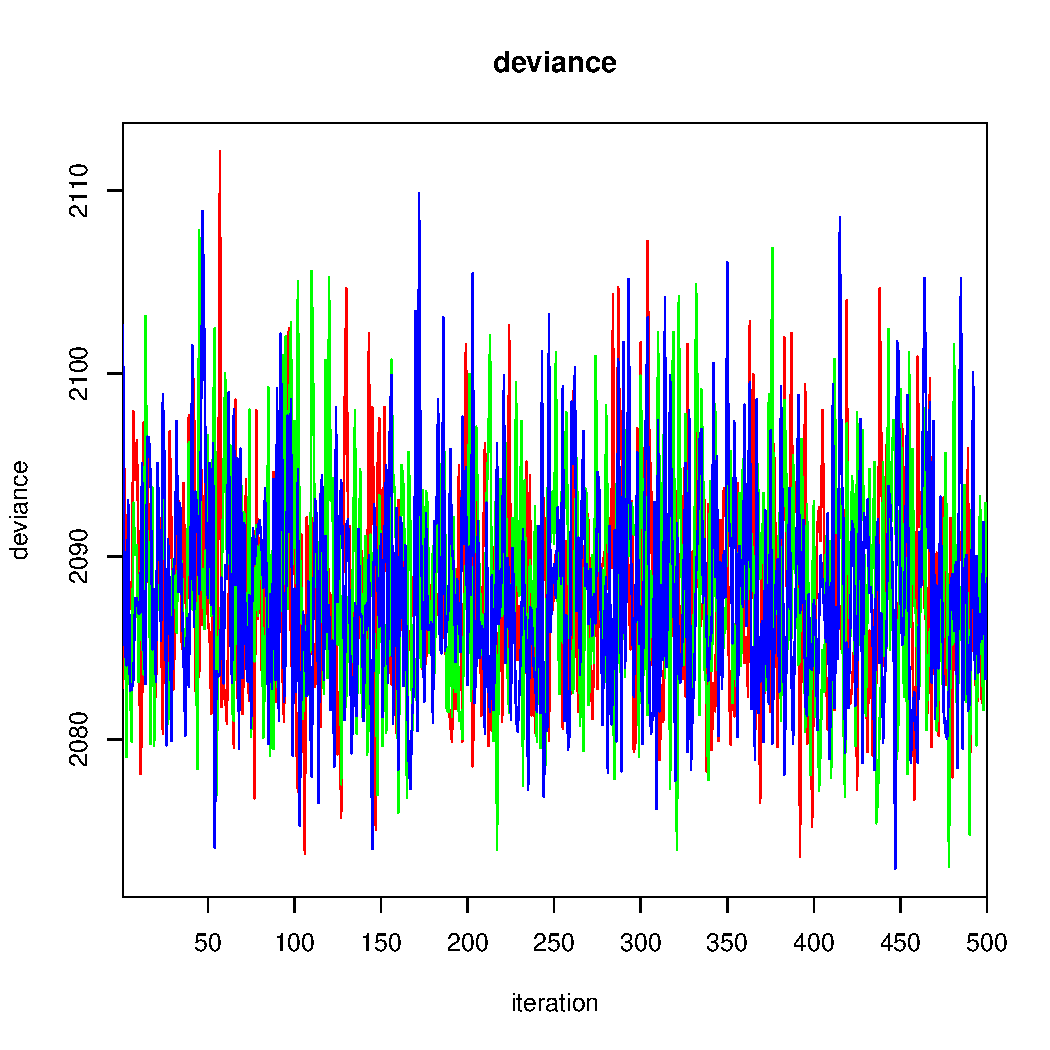
\includegraphics[width=.15\columnwidth]{../graphs/traceplots/2003d0v_1.pdf} &
                        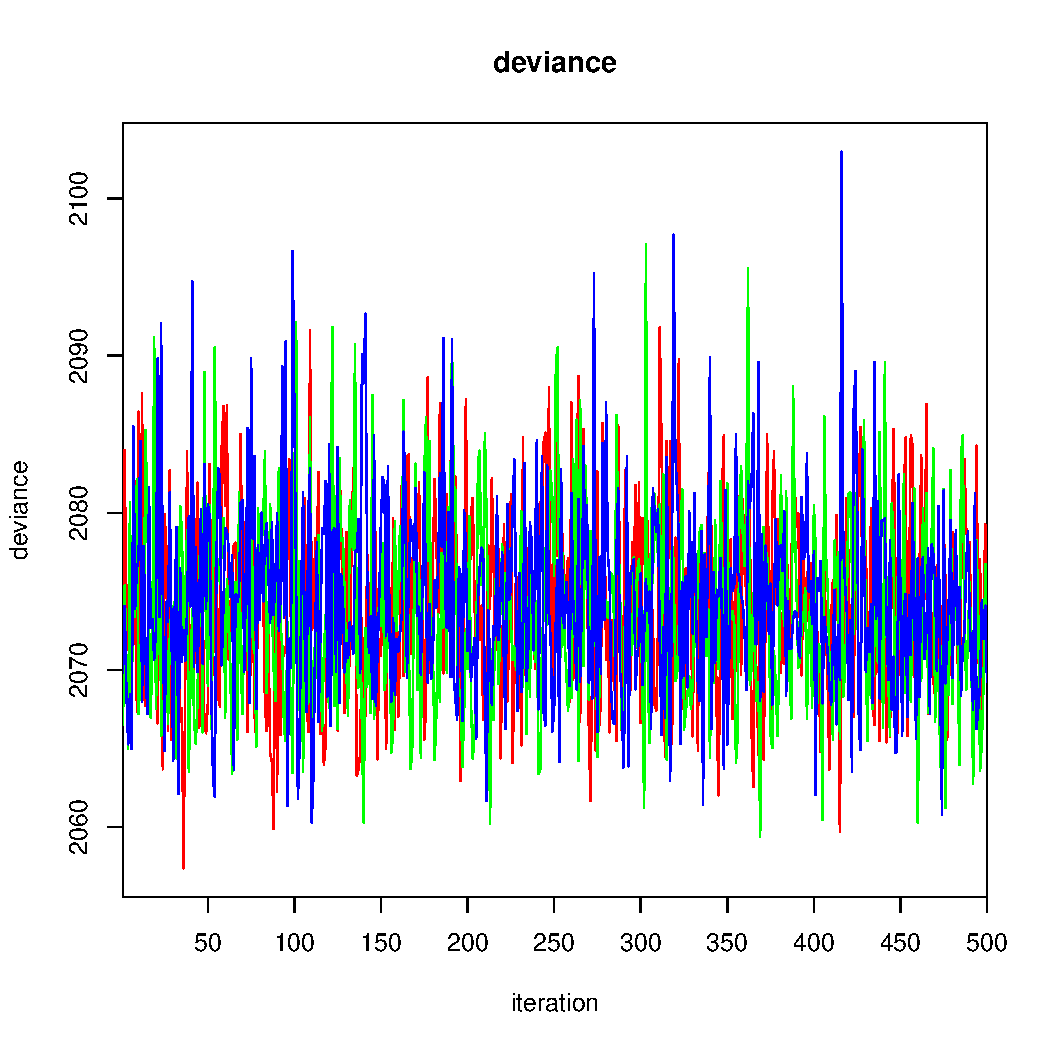
\includegraphics[width=.15\columnwidth]{../graphs/traceplots/2003d0vbar_1.pdf} &
                         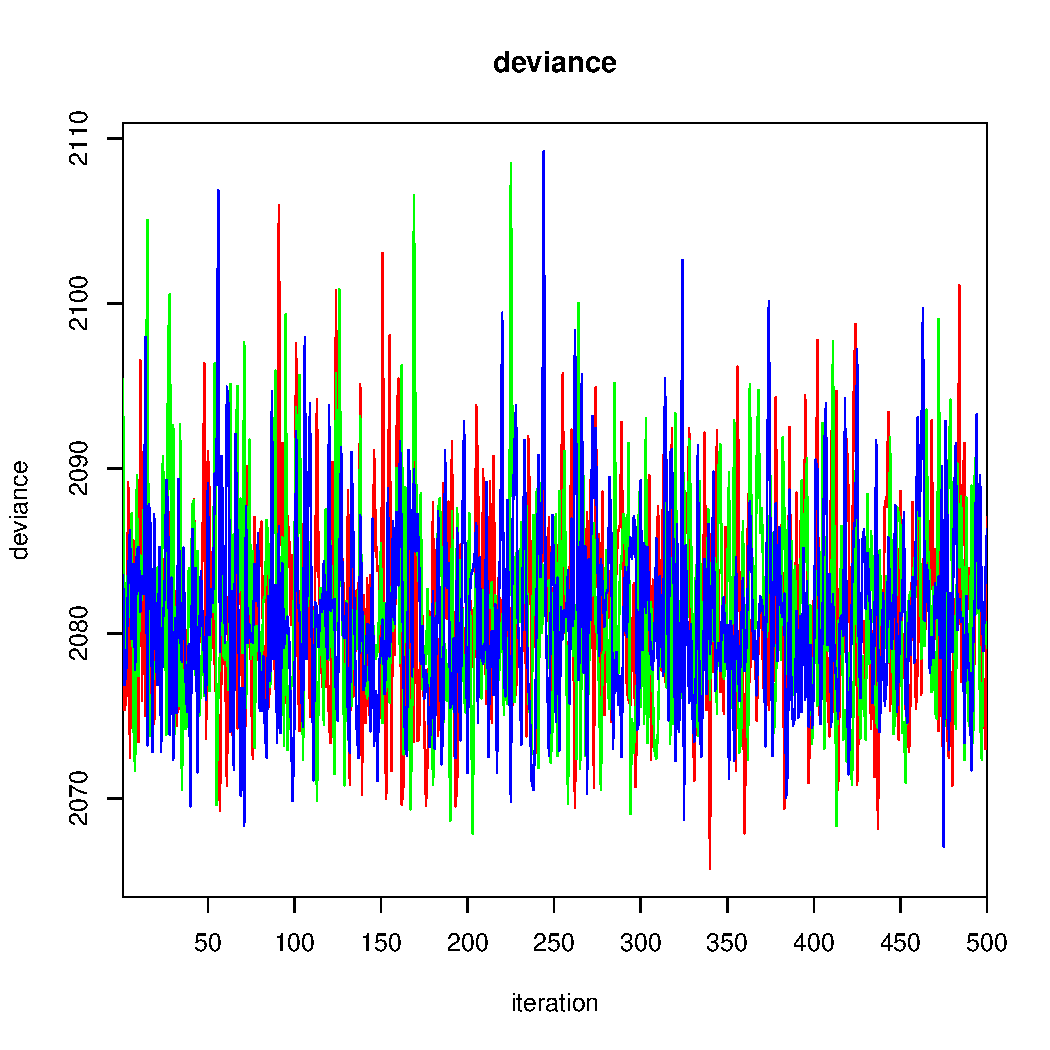
\includegraphics[width=.15\columnwidth]{../graphs/traceplots/2003d0wbar_1.pdf} \\
    $\lambda_{PAN}$   & 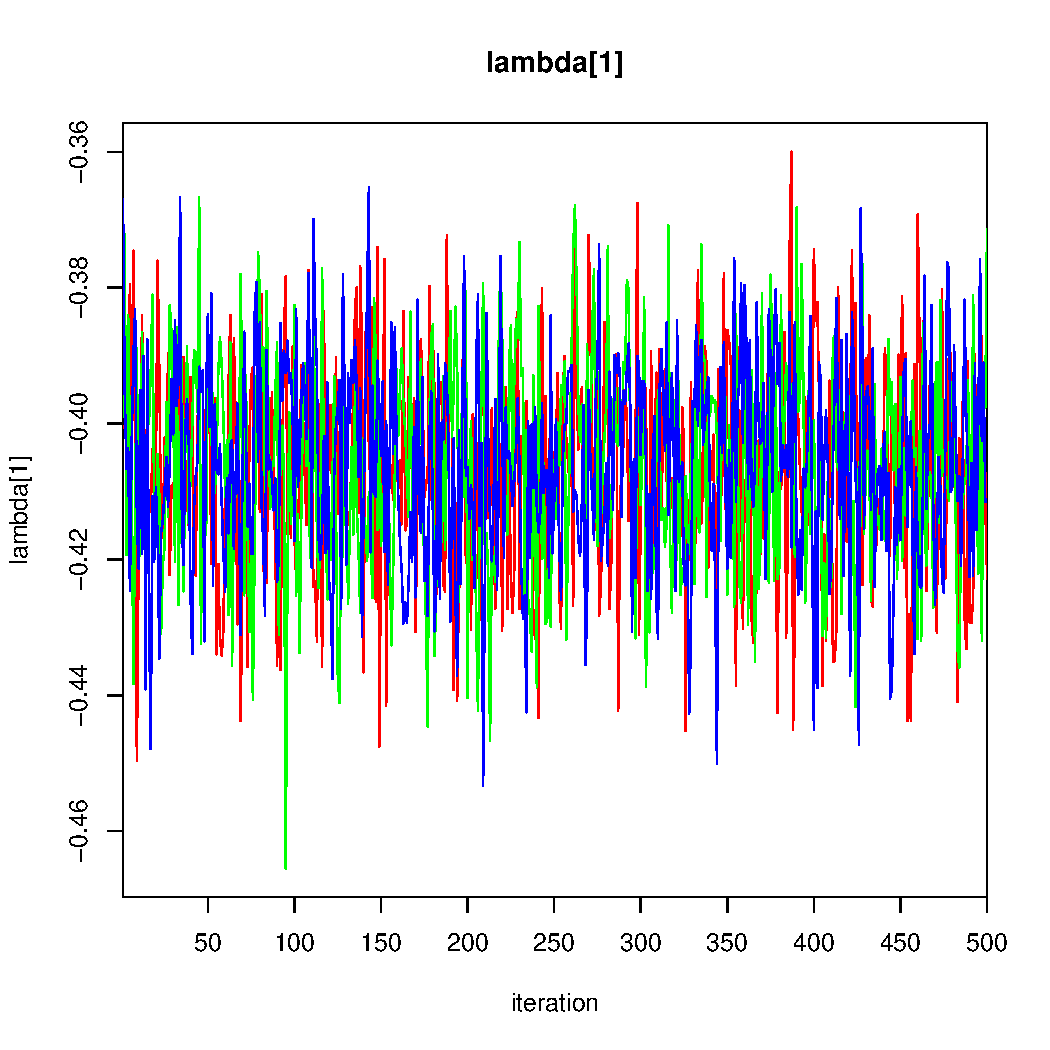
\includegraphics[width=.15\columnwidth]{../graphs/traceplots/2003d0v_2.pdf} &
                        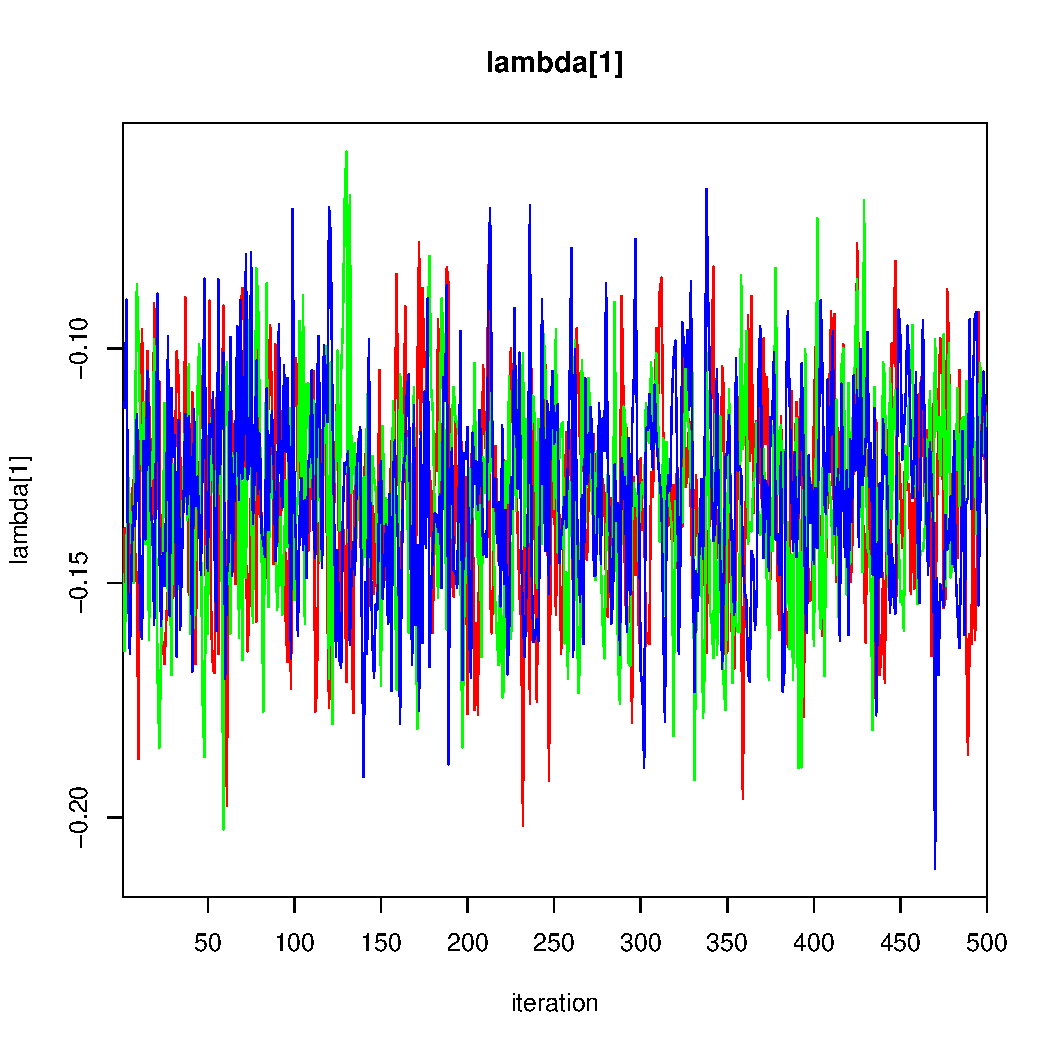
\includegraphics[width=.15\columnwidth]{../graphs/traceplots/2003d0vbar_2.pdf} &
                         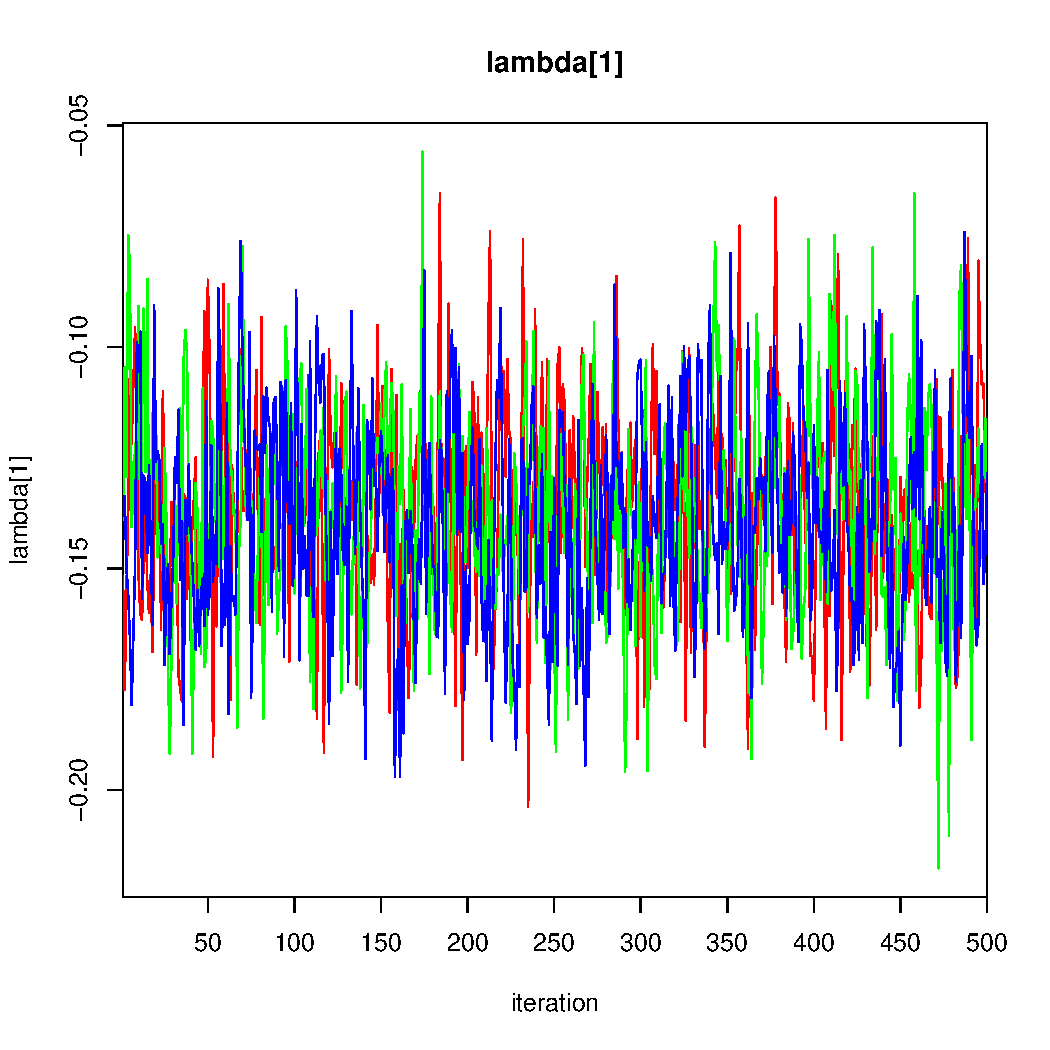
\includegraphics[width=.15\columnwidth]{../graphs/traceplots/2003d0wbar_2.pdf} \\
    $\lambda_{PRD}$   & 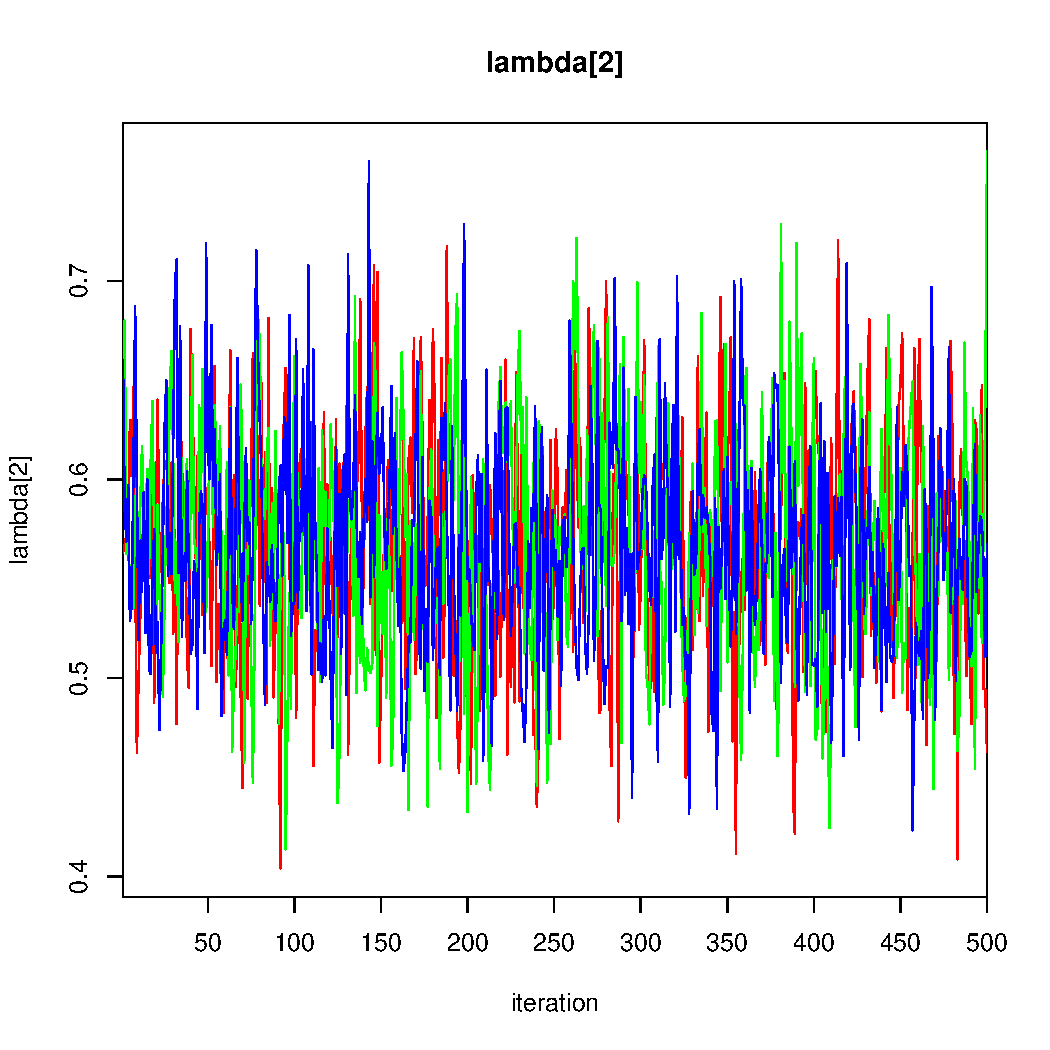
\includegraphics[width=.15\columnwidth]{../graphs/traceplots/2003d0v_3.pdf} &
                        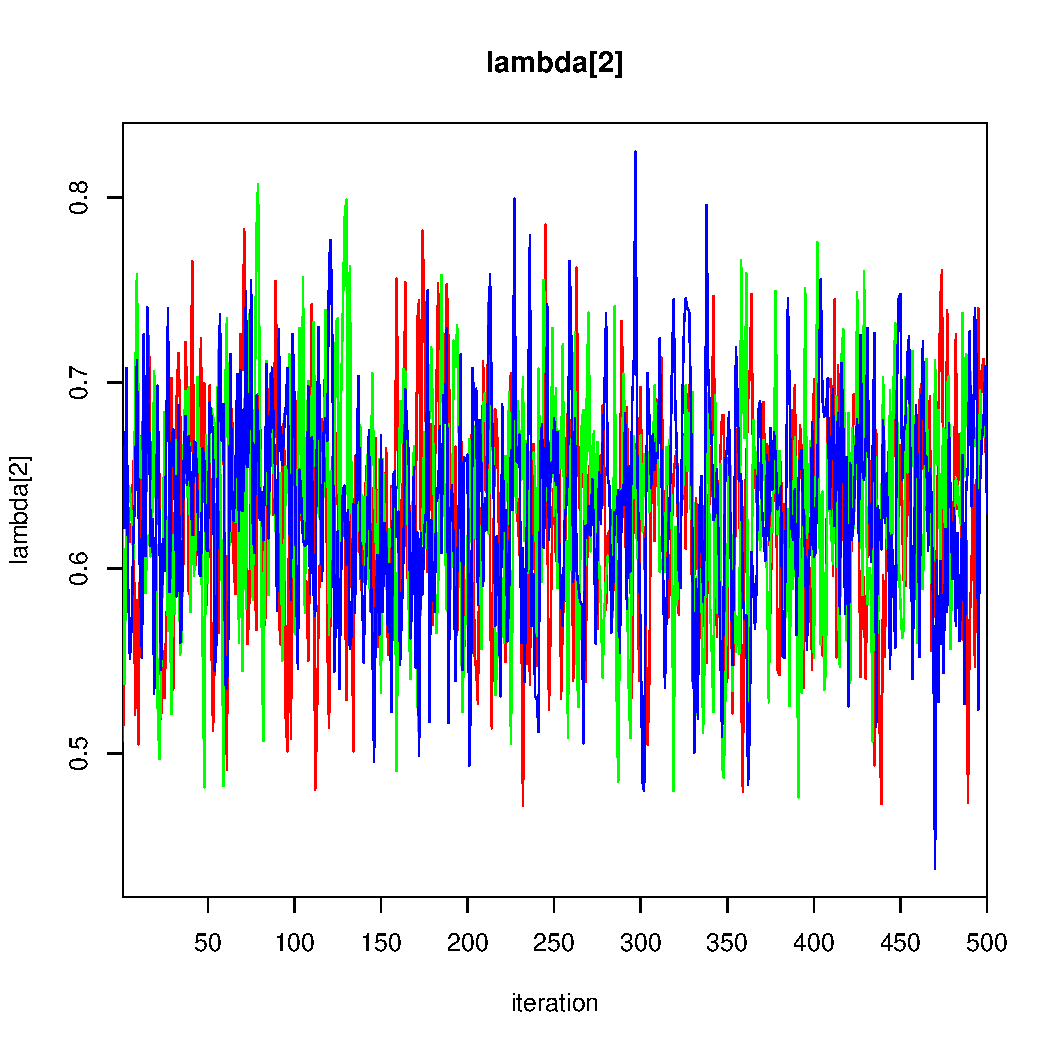
\includegraphics[width=.15\columnwidth]{../graphs/traceplots/2003d0vbar_3.pdf} &
                         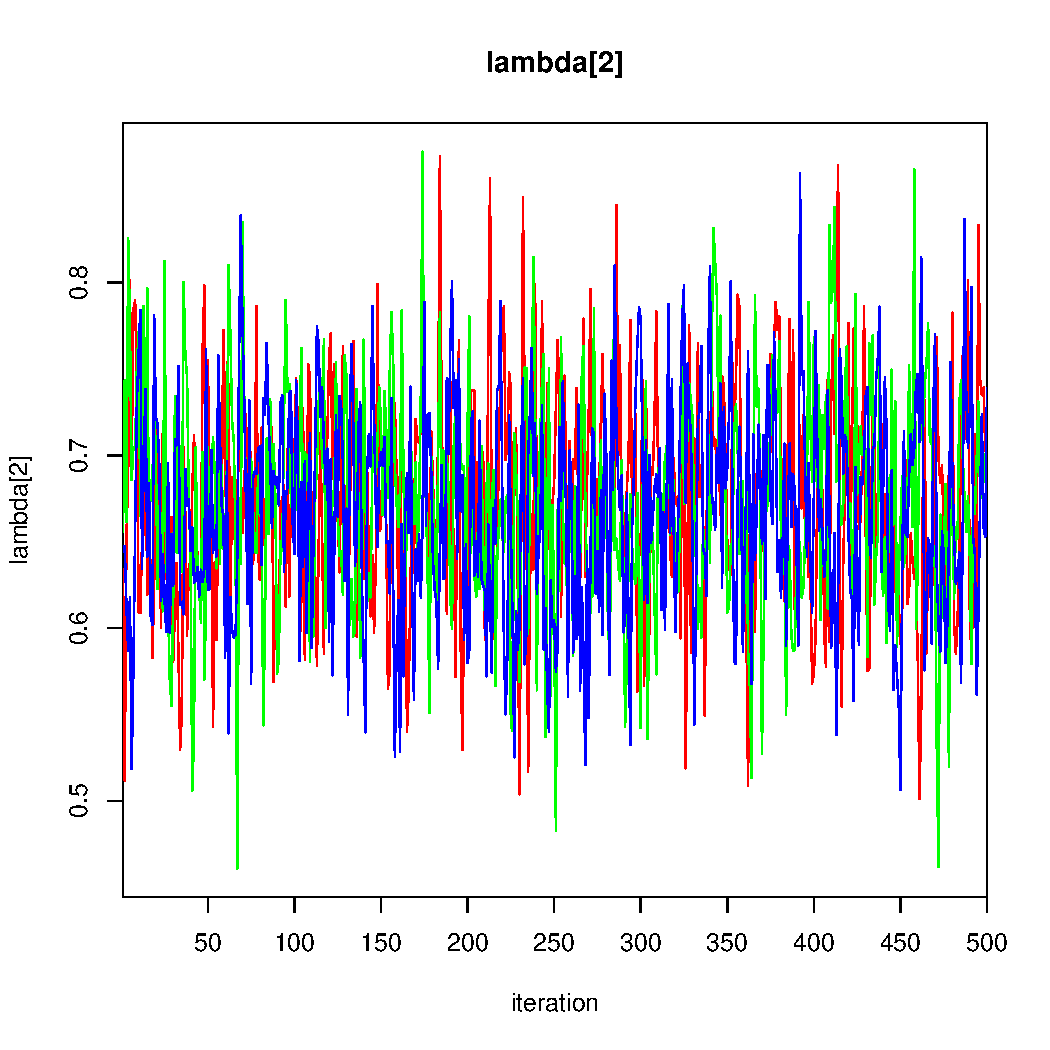
\includegraphics[width=.15\columnwidth]{../graphs/traceplots/2003d0wbar_3.pdf} \\
    $\lambda_{Green}$  & 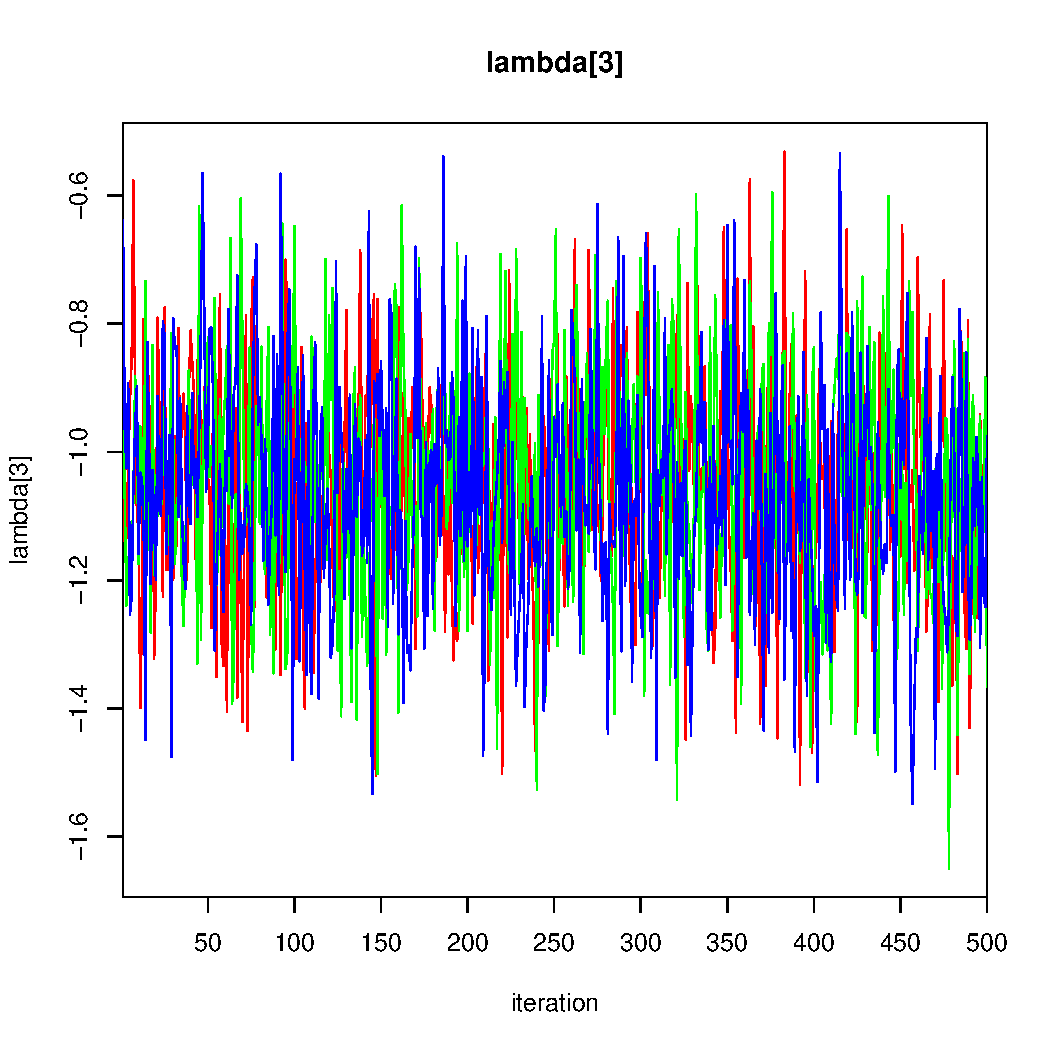
\includegraphics[width=.15\columnwidth]{../graphs/traceplots/2003d0v_4.pdf} &
                        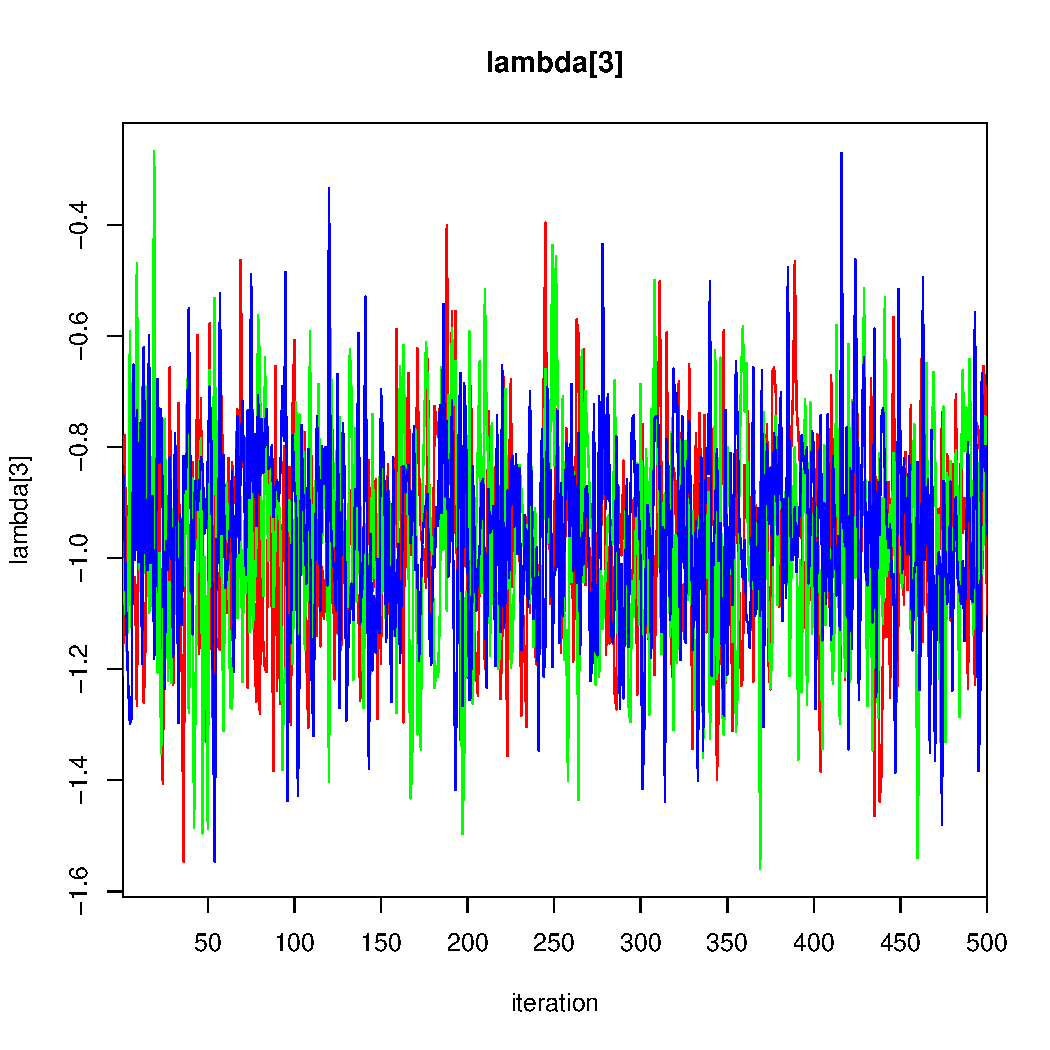
\includegraphics[width=.15\columnwidth]{../graphs/traceplots/2003d0vbar_4.pdf} &
                         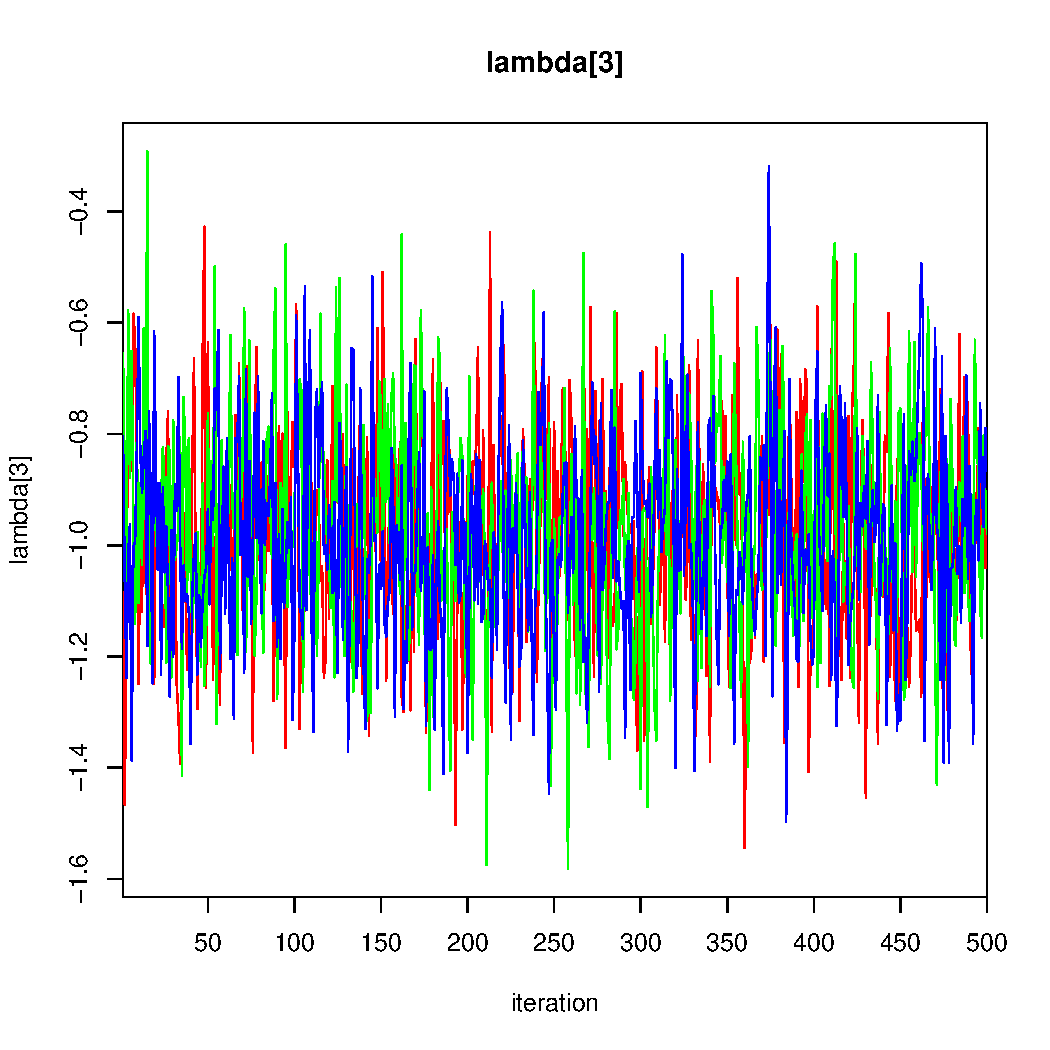
\includegraphics[width=.15\columnwidth]{../graphs/traceplots/2003d0wbar_4.pdf} \\
    $\lambda_{MC}$    & 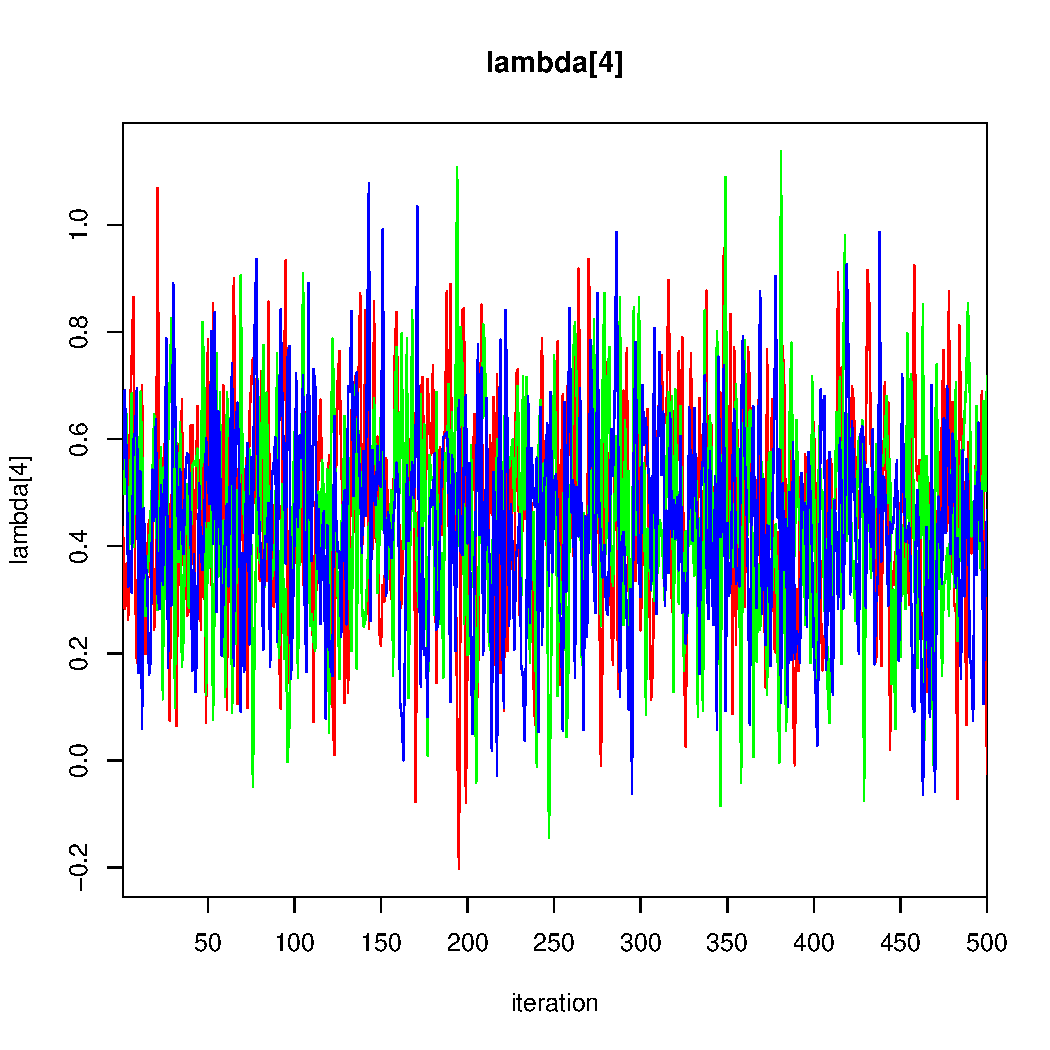
\includegraphics[width=.15\columnwidth]{../graphs/traceplots/2003d0v_5.pdf} &
                        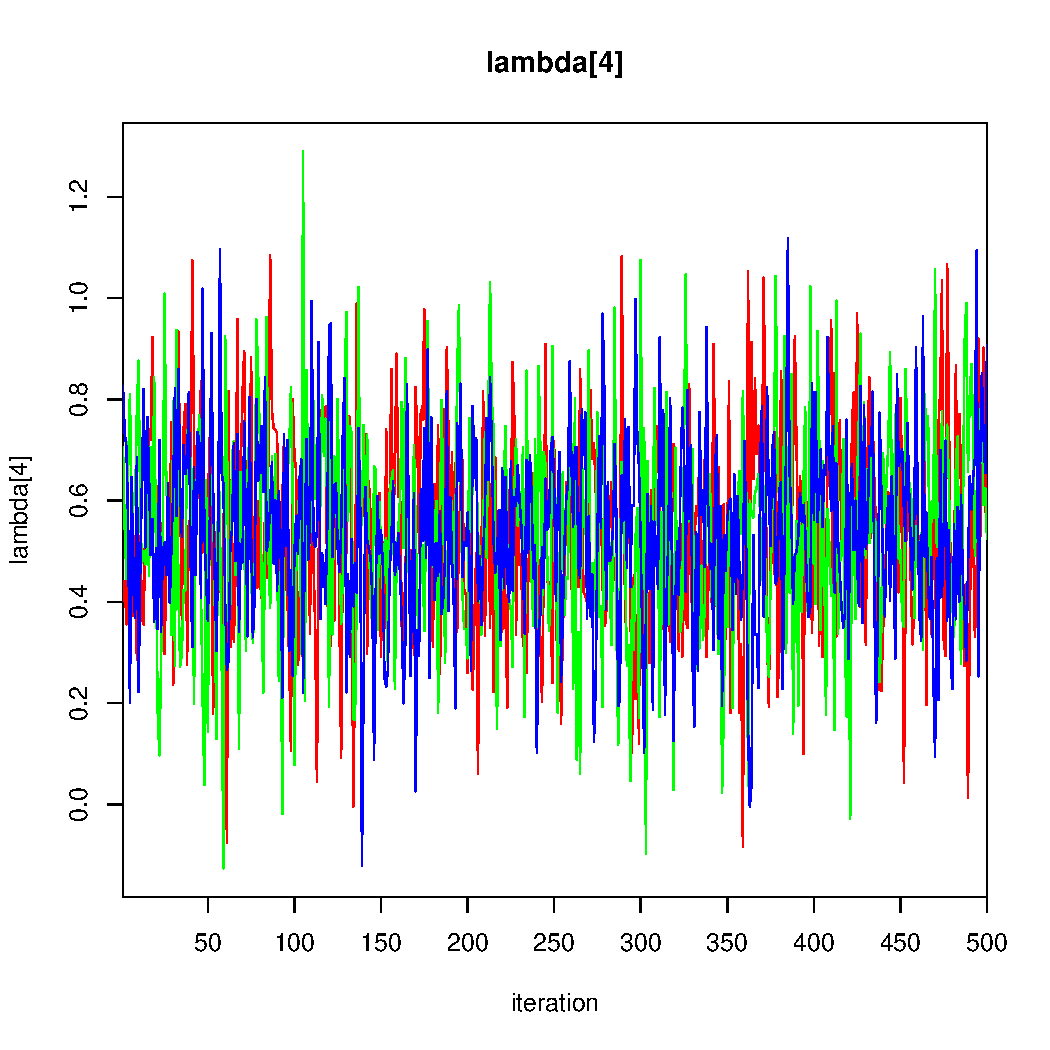
\includegraphics[width=.15\columnwidth]{../graphs/traceplots/2003d0vbar_5.pdf} &
                         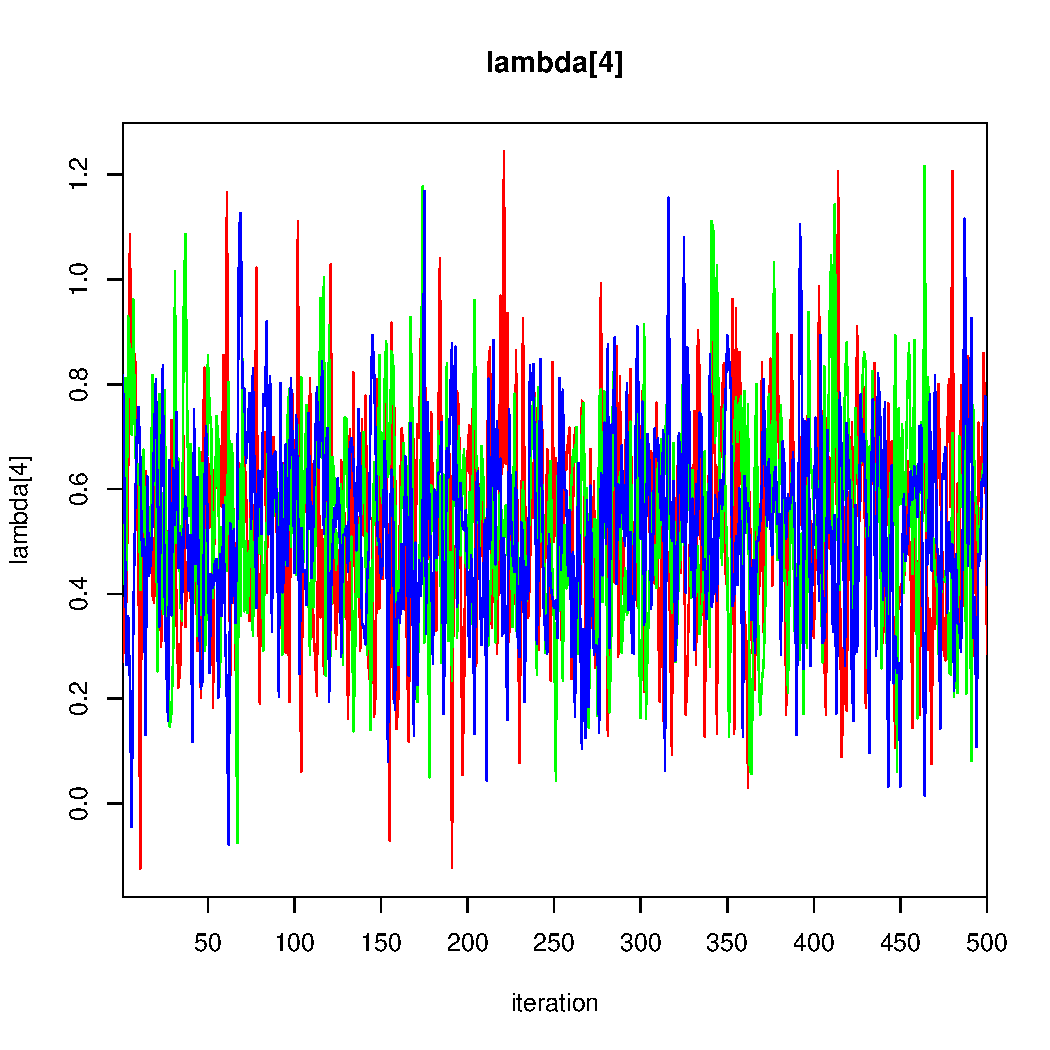
\includegraphics[width=.15\columnwidth]{../graphs/traceplots/2003d0wbar_5.pdf} \\
    % $\lambda_{morena}$ & 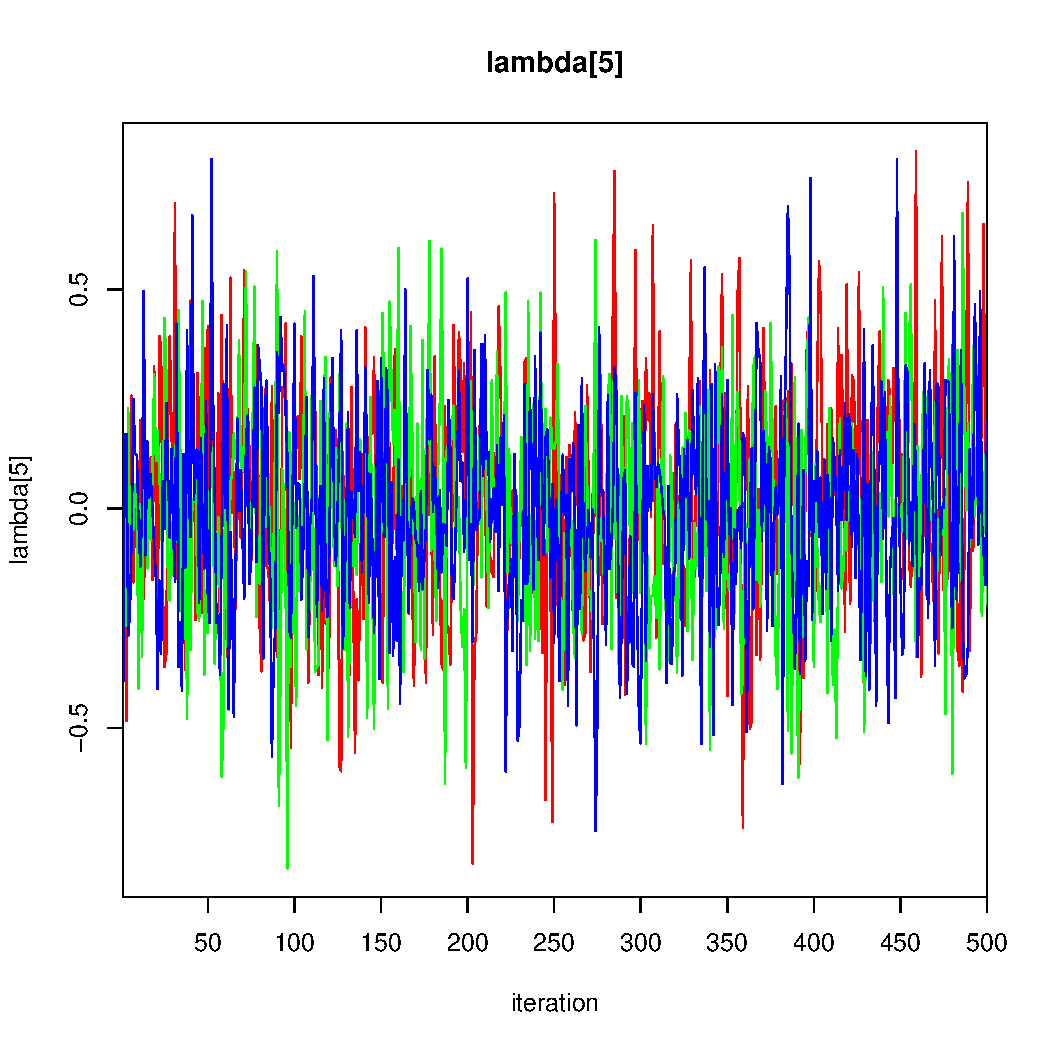
\includegraphics[width=.15\columnwidth]{../graphs/traceplots/2003d0v_6.pdf} &
    %                     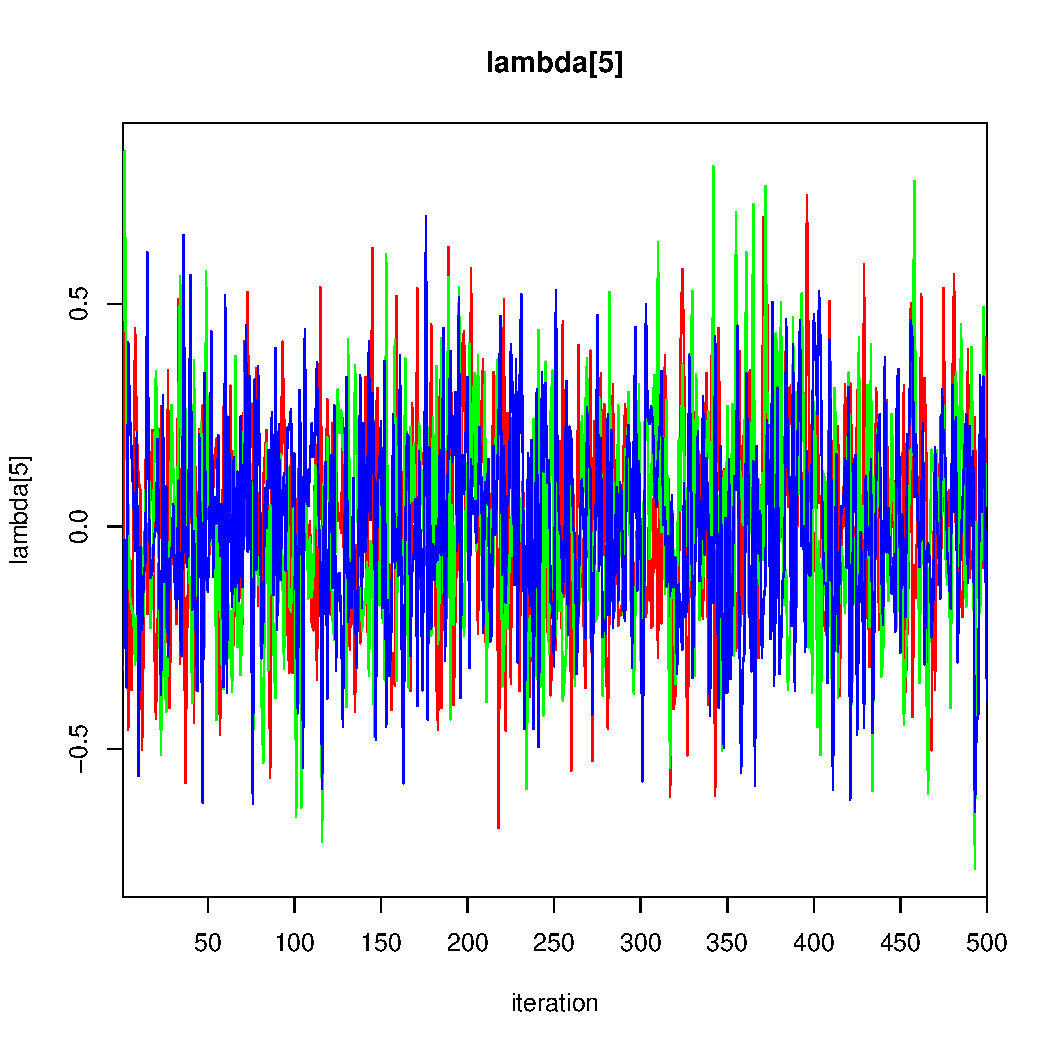
\includegraphics[width=.15\columnwidth]{../graphs/traceplots/2003d0vbar_6.pdf} &
    %                      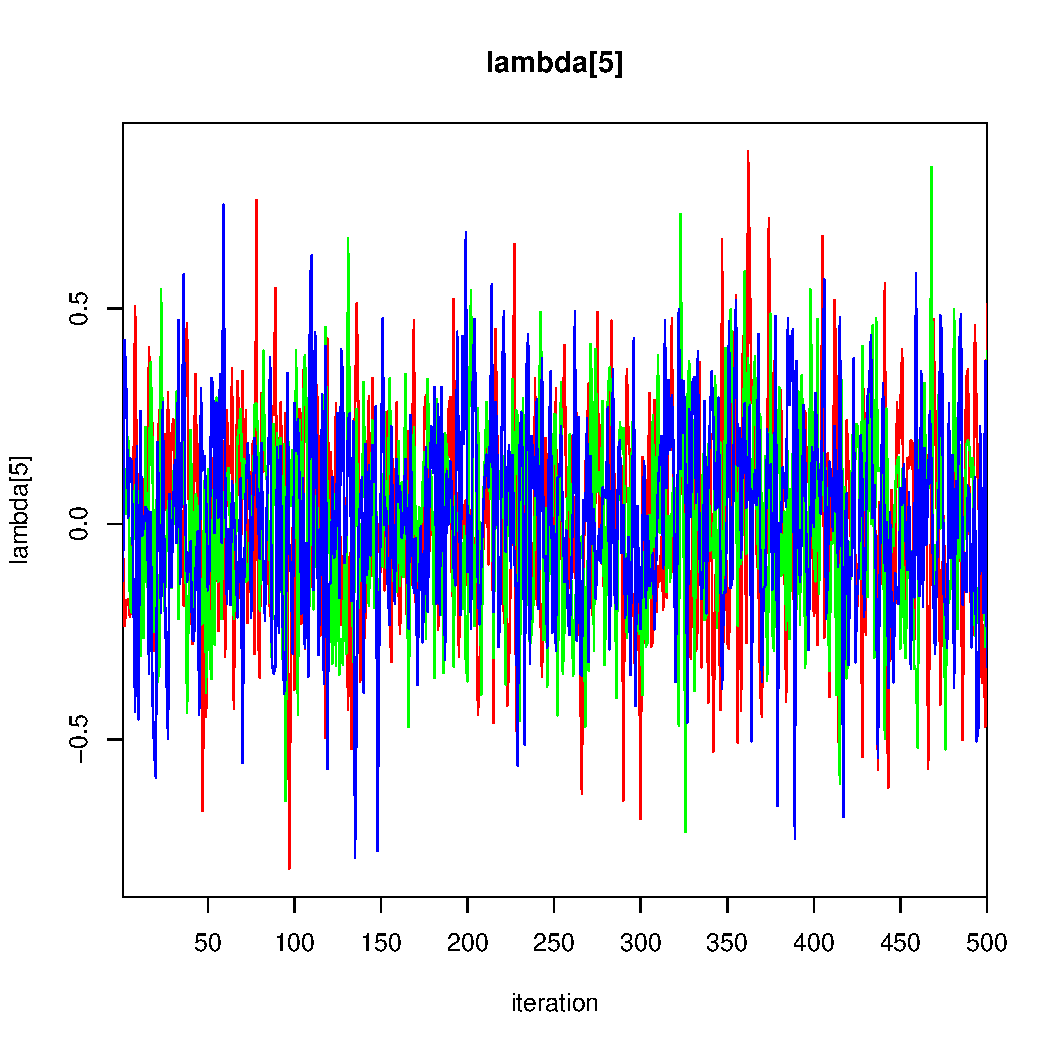
\includegraphics[width=.15\columnwidth]{../graphs/traceplots/2003d0wbar_6.pdf} \\
    $\rho$           & 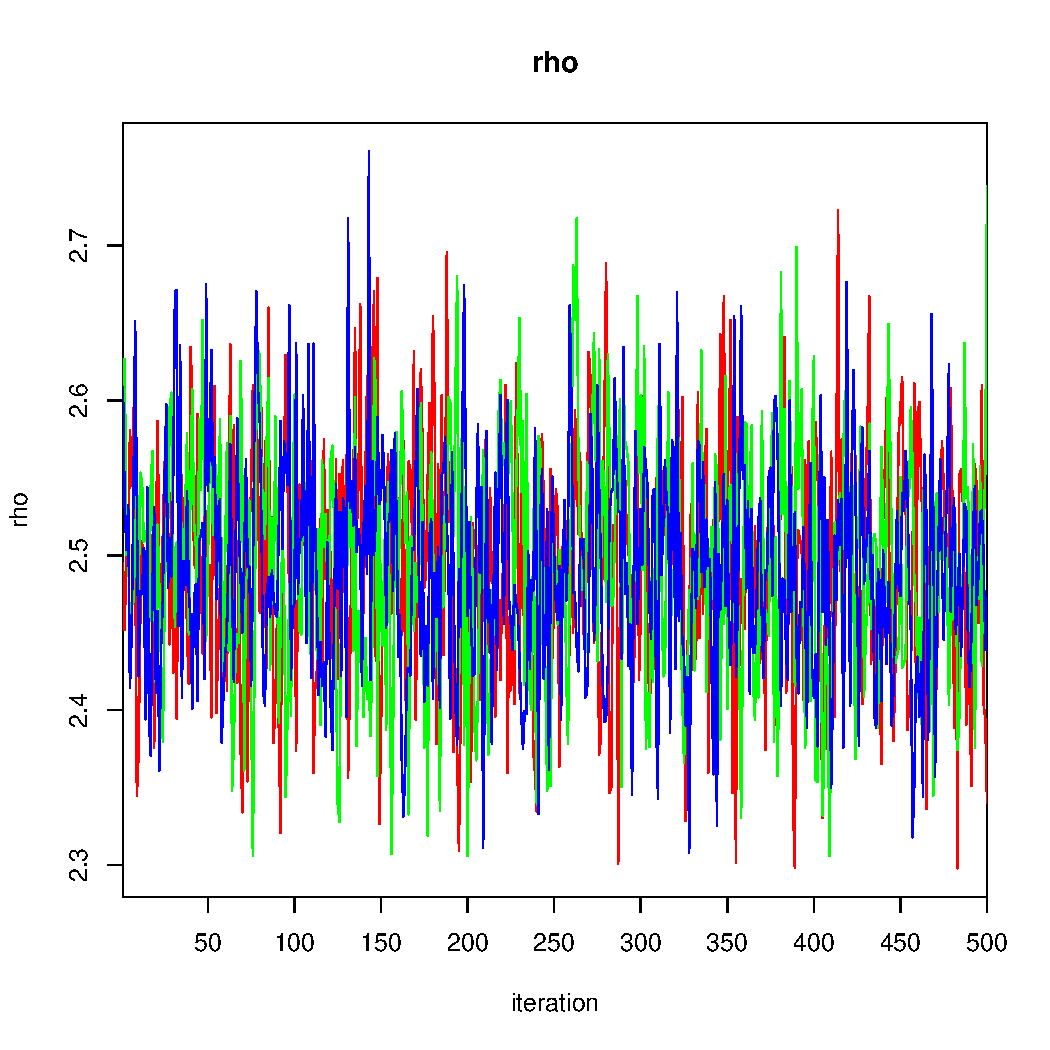
\includegraphics[width=.15\columnwidth]{../graphs/traceplots/2003d0v_7.pdf} &
                        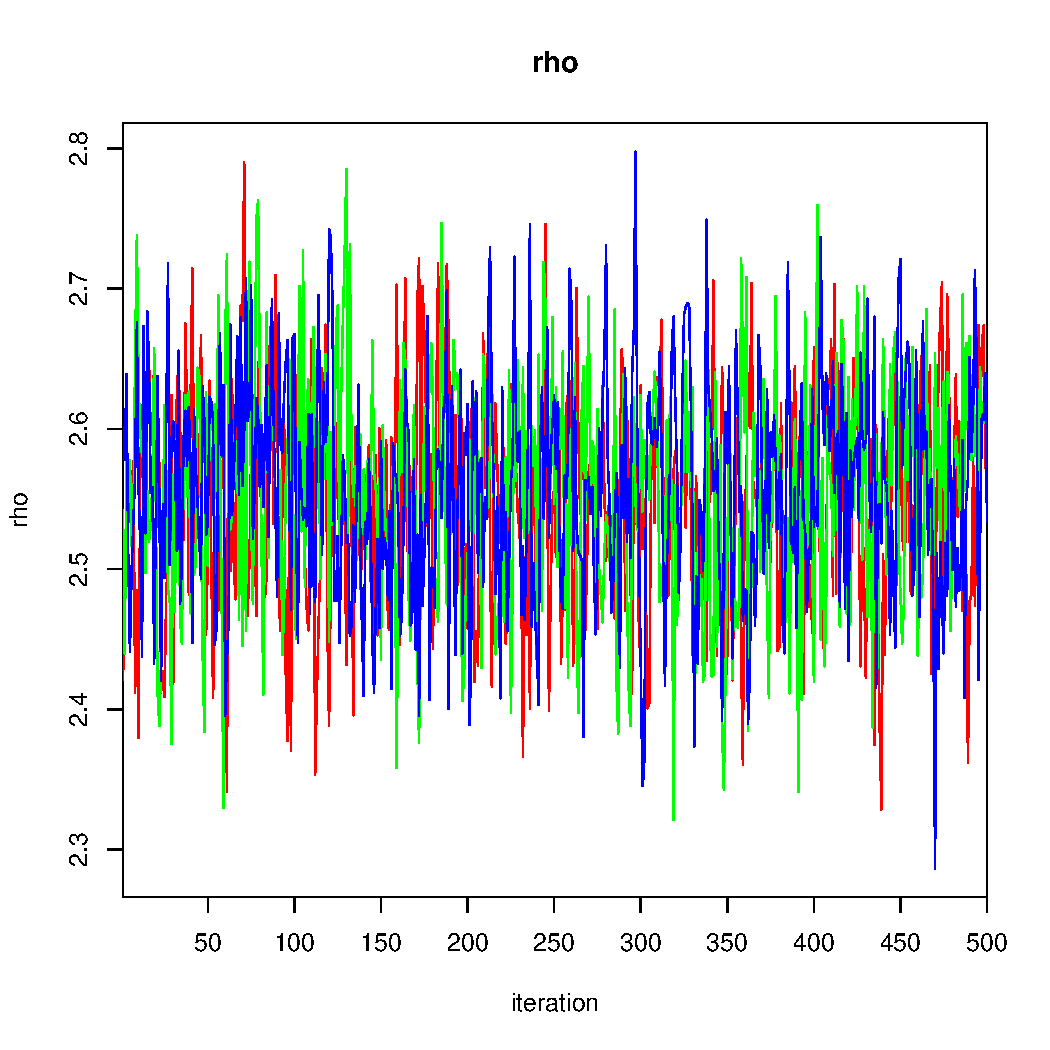
\includegraphics[width=.15\columnwidth]{../graphs/traceplots/2003d0vbar_7.pdf} &
                         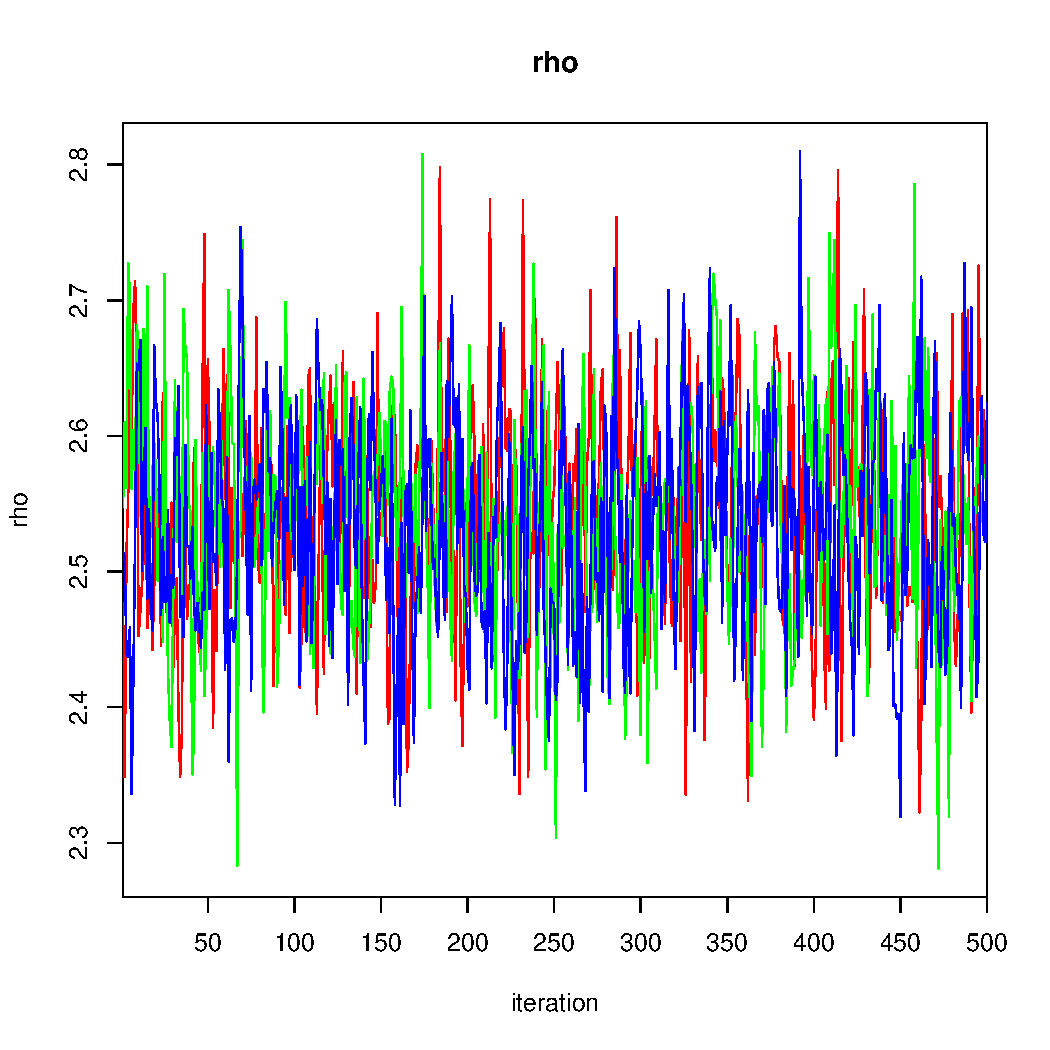
\includegraphics[width=.15\columnwidth]{../graphs/traceplots/2003d0wbar_7.pdf} \\
\end{tabular}
\caption{Three-chain traceplots for 2003 with hypothetical map}
\end{table}

\begin{table}
\centering
\begin{tabular}{cccc}
                     & $\texttt{v}$ & $\bar{\texttt{v}}$ & $\bar{\texttt{w}}$ \\ 
    Dev.             & 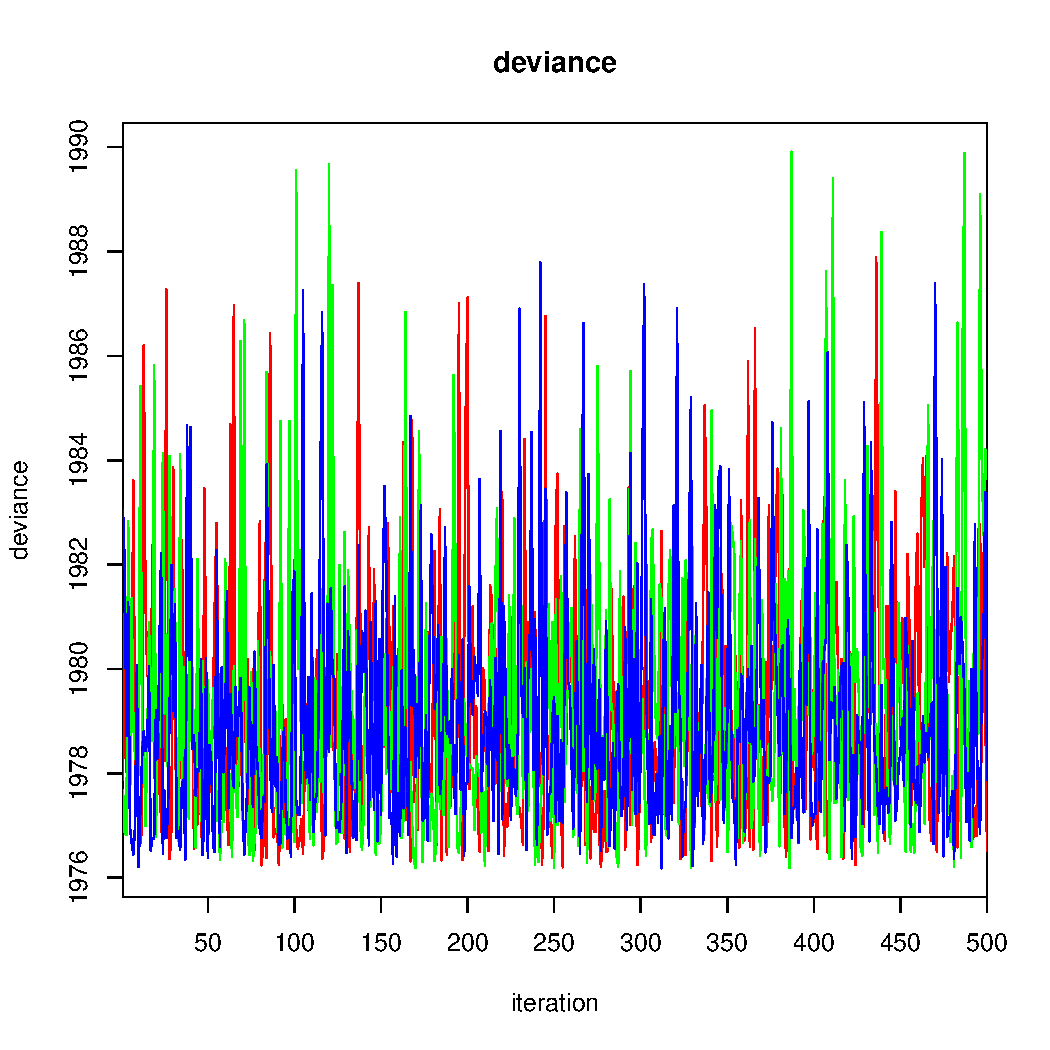
\includegraphics[width=.15\columnwidth]{../graphs/traceplots/2006d0v_1.pdf} &
                        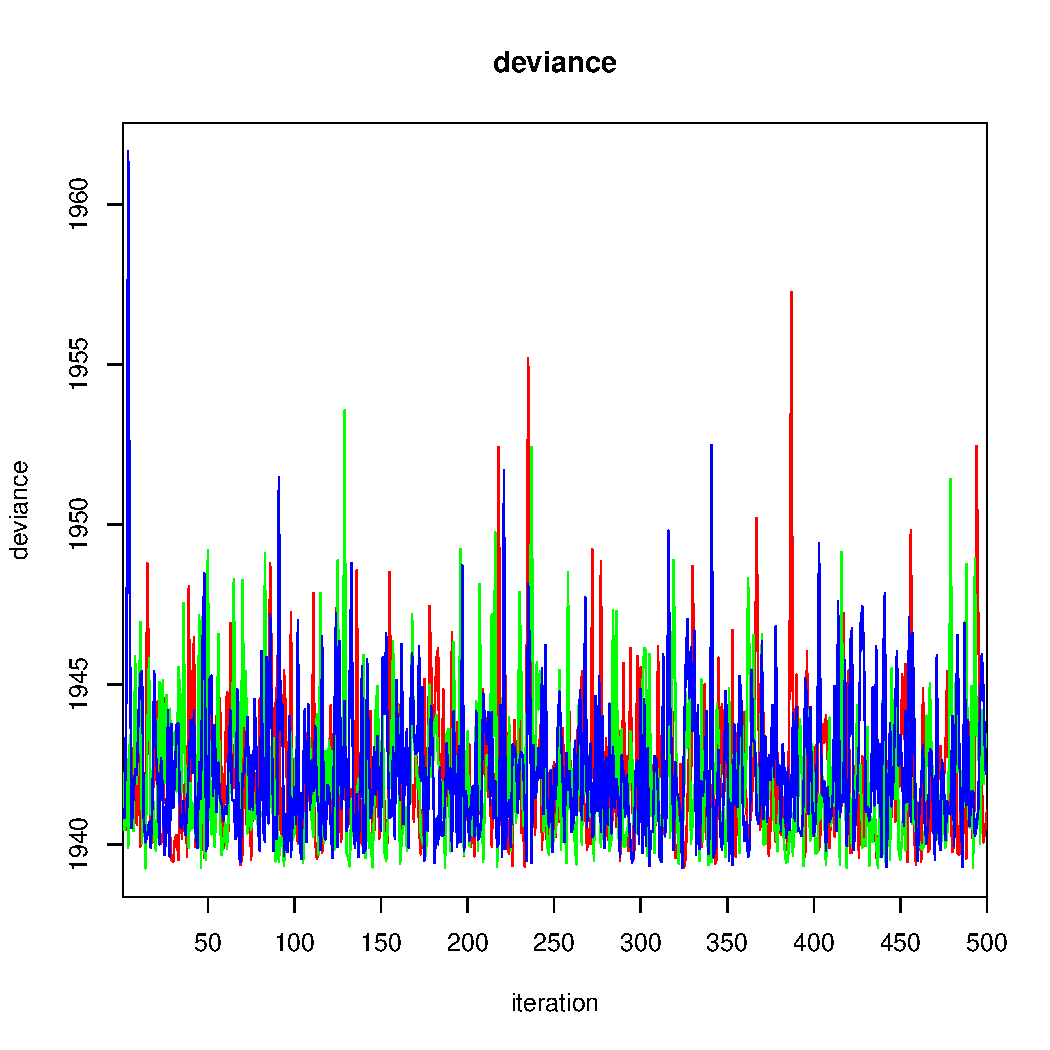
\includegraphics[width=.15\columnwidth]{../graphs/traceplots/2006d0vbar_1.pdf} &
                         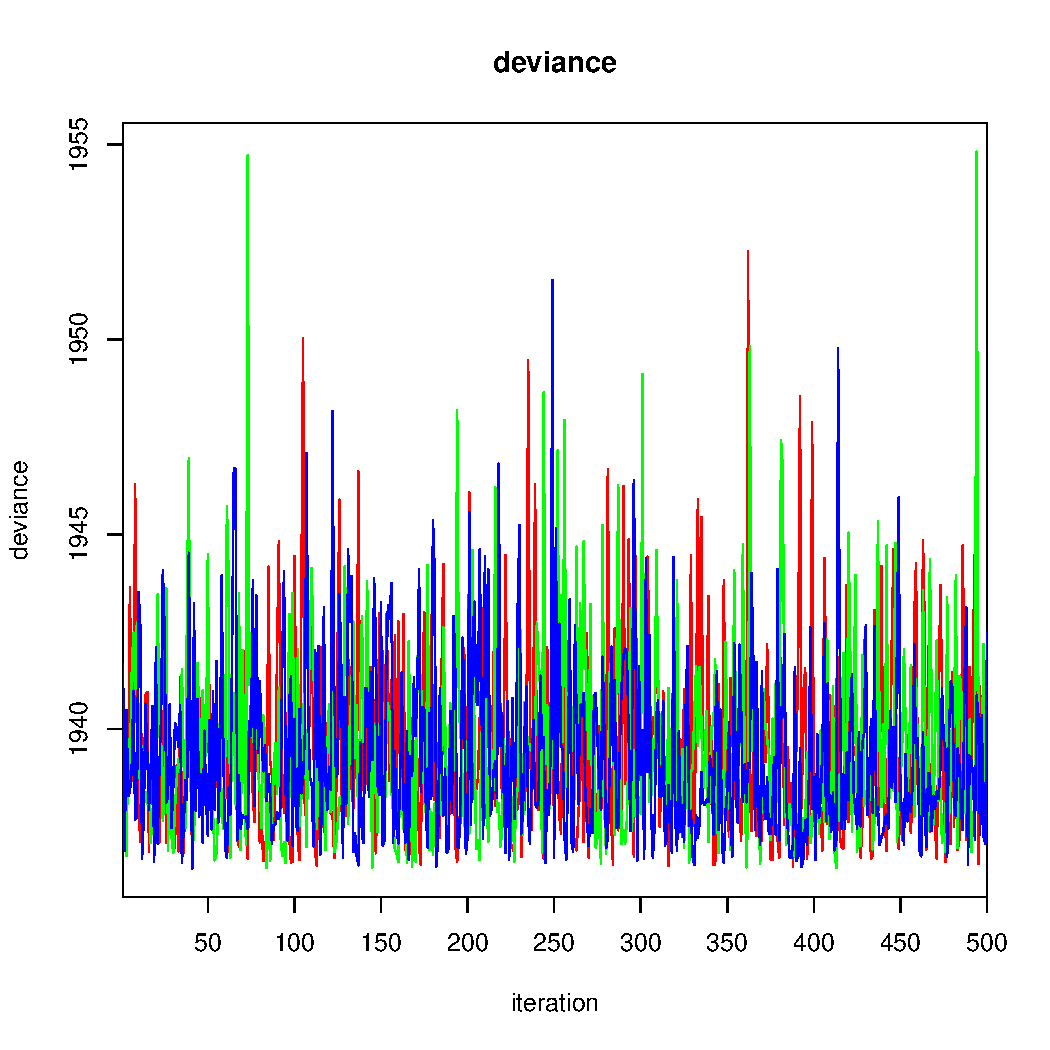
\includegraphics[width=.15\columnwidth]{../graphs/traceplots/2006d0wbar_1.pdf} \\
    $\lambda_{PAN}$   & 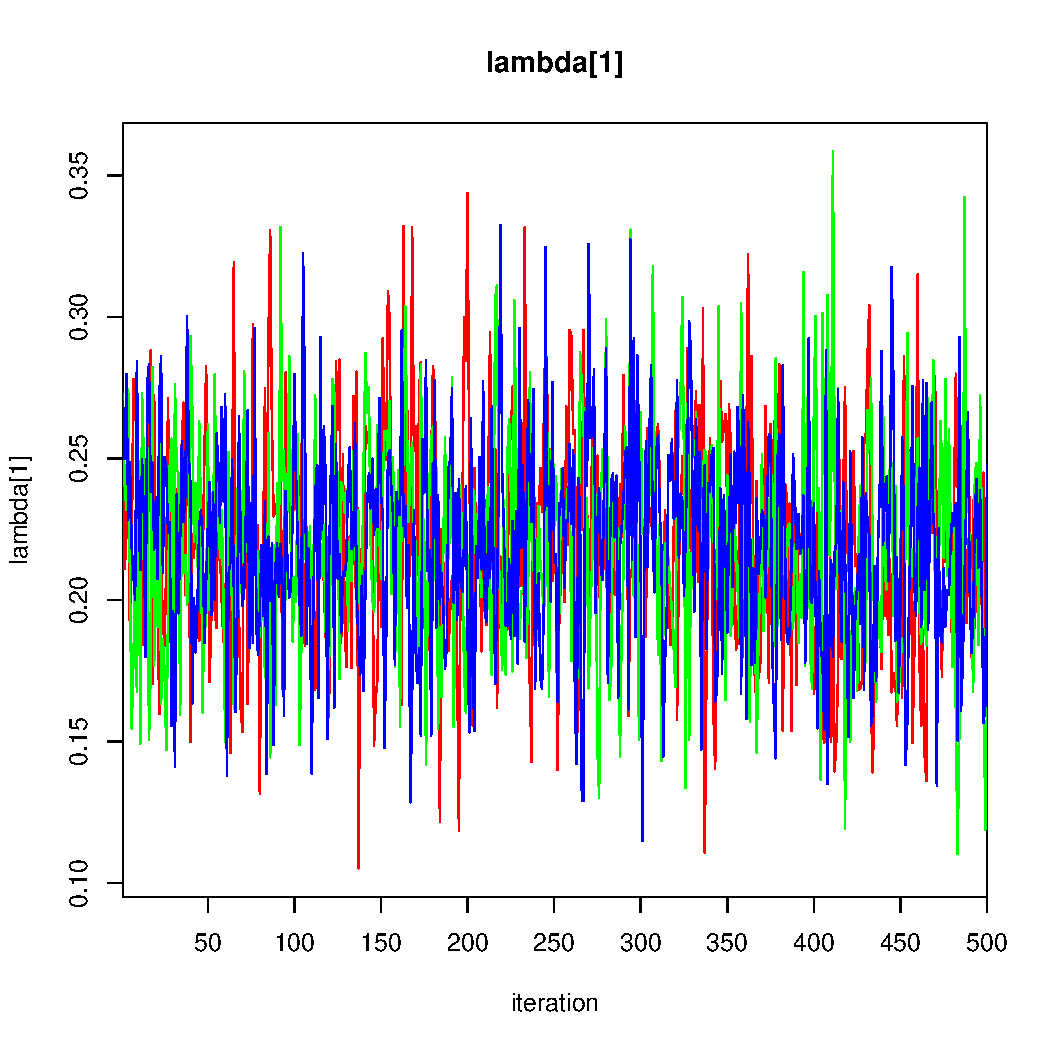
\includegraphics[width=.15\columnwidth]{../graphs/traceplots/2006d0v_2.pdf} &
                        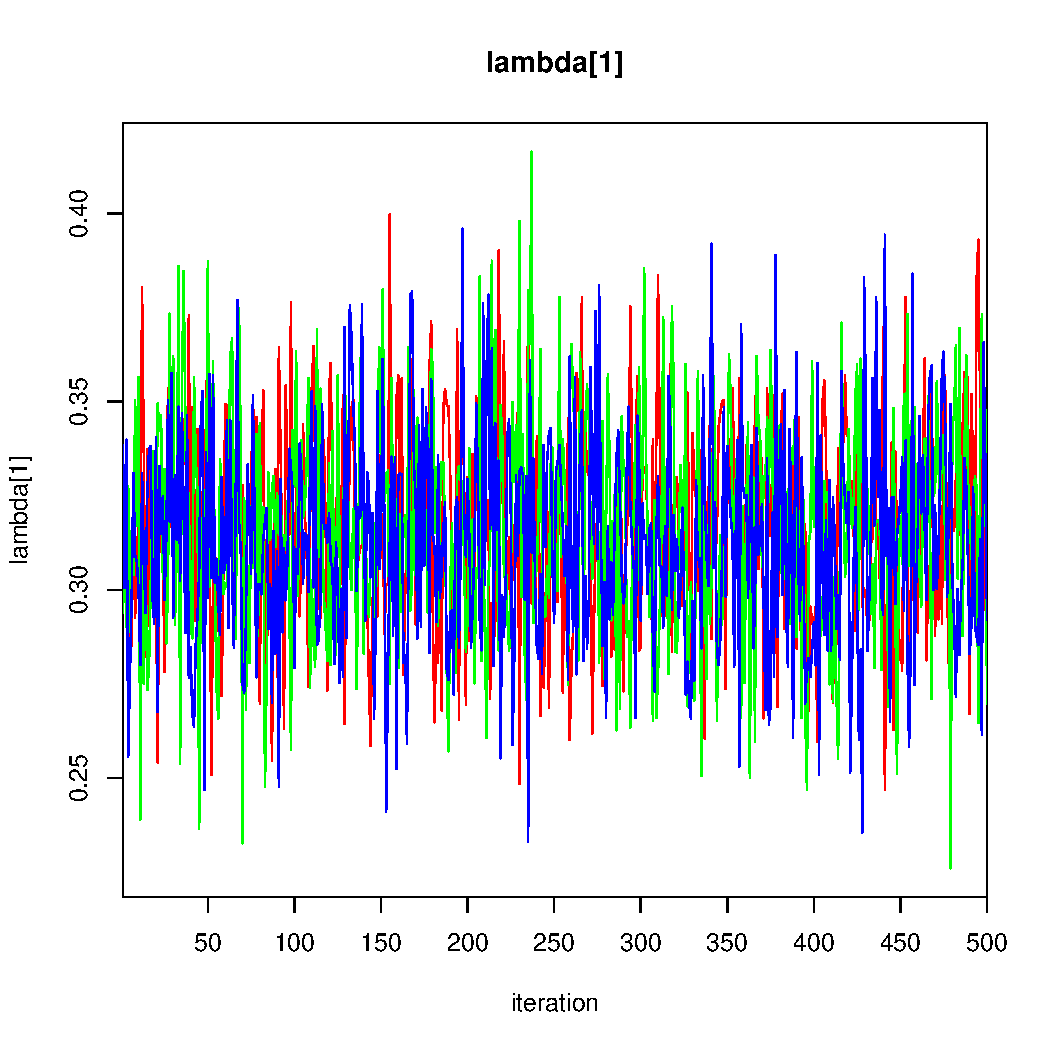
\includegraphics[width=.15\columnwidth]{../graphs/traceplots/2006d0vbar_2.pdf} &
                         \includegraphics[width=.15\columnwidth]{../graphs/traceplots/2006d0wbar_2.pdf} \\
    $\lambda_{PRD}$   & \includegraphics[width=.15\columnwidth]{../graphs/traceplots/2006d0v_3.pdf} &
                        \includegraphics[width=.15\columnwidth]{../graphs/traceplots/2006d0vbar_3.pdf} &
                         \includegraphics[width=.15\columnwidth]{../graphs/traceplots/2006d0wbar_3.pdf} \\
    % $\lambda_{Green}$  & \includegraphics[width=.15\columnwidth]{../graphs/traceplots/2006d0v_4.pdf} &
    %                     \includegraphics[width=.15\columnwidth]{../graphs/traceplots/2006d0vbar_4.pdf} &
    %                      \includegraphics[width=.15\columnwidth]{../graphs/traceplots/2006d0wbar_4.pdf} \\
    % $\lambda_{MC}$    & \includegraphics[width=.15\columnwidth]{../graphs/traceplots/2006d0v_5.pdf} &
    %                     \includegraphics[width=.15\columnwidth]{../graphs/traceplots/2006d0vbar_5.pdf} &
    %                      \includegraphics[width=.15\columnwidth]{../graphs/traceplots/2006d0wbar_5.pdf} \\
    % $\lambda_{morena}$ & \includegraphics[width=.15\columnwidth]{../graphs/traceplots/2006d0v_6.pdf} &
    %                     \includegraphics[width=.15\columnwidth]{../graphs/traceplots/2006d0vbar_6.pdf} &
    %                      \includegraphics[width=.15\columnwidth]{../graphs/traceplots/2006d0wbar_6.pdf} \\
    $\rho$           & \includegraphics[width=.15\columnwidth]{../graphs/traceplots/2006d0v_7.pdf} &
                        \includegraphics[width=.15\columnwidth]{../graphs/traceplots/2006d0vbar_7.pdf} &
                         \includegraphics[width=.15\columnwidth]{../graphs/traceplots/2006d0wbar_7.pdf} \\
\end{tabular}
\caption{Three-chain traceplots for 2006 with status quo map}
\end{table}

\begin{table}
\centering
\begin{tabular}{cccc}
                     & $\texttt{v}$ & $\bar{\texttt{v}}$ & $\bar{\texttt{w}}$ \\ 
    Dev.             & \includegraphics[width=.15\columnwidth]{../graphs/traceplots/2009d0v_1.pdf} &
                        \includegraphics[width=.15\columnwidth]{../graphs/traceplots/2009d0vbar_1.pdf} &
                         \includegraphics[width=.15\columnwidth]{../graphs/traceplots/2009d0wbar_1.pdf} \\
    $\lambda_{PAN}$   & \includegraphics[width=.15\columnwidth]{../graphs/traceplots/2009d0v_2.pdf} &
                        \includegraphics[width=.15\columnwidth]{../graphs/traceplots/2009d0vbar_2.pdf} &
                         \includegraphics[width=.15\columnwidth]{../graphs/traceplots/2009d0wbar_2.pdf} \\
    $\lambda_{PRD}$   & \includegraphics[width=.15\columnwidth]{../graphs/traceplots/2009d0v_3.pdf} &
                        \includegraphics[width=.15\columnwidth]{../graphs/traceplots/2009d0vbar_3.pdf} &
                         \includegraphics[width=.15\columnwidth]{../graphs/traceplots/2009d0wbar_3.pdf} \\
    $\lambda_{Green}$  & \includegraphics[width=.15\columnwidth]{../graphs/traceplots/2009d0v_4.pdf} &
                        \includegraphics[width=.15\columnwidth]{../graphs/traceplots/2009d0vbar_4.pdf} &
                         \includegraphics[width=.15\columnwidth]{../graphs/traceplots/2009d0wbar_4.pdf} \\
    $\lambda_{MC}$    & \includegraphics[width=.15\columnwidth]{../graphs/traceplots/2009d0v_5.pdf} &
                        \includegraphics[width=.15\columnwidth]{../graphs/traceplots/2009d0vbar_5.pdf} &
                         \includegraphics[width=.15\columnwidth]{../graphs/traceplots/2009d0wbar_5.pdf} \\
    % $\lambda_{morena}$ & \includegraphics[width=.15\columnwidth]{../graphs/traceplots/2009d0v_6.pdf} &
    %                     \includegraphics[width=.15\columnwidth]{../graphs/traceplots/2009d0vbar_6.pdf} &
    %                      \includegraphics[width=.15\columnwidth]{../graphs/traceplots/2009d0wbar_6.pdf} \\
    $\rho$           & \includegraphics[width=.15\columnwidth]{../graphs/traceplots/2009d0v_7.pdf} &
                        \includegraphics[width=.15\columnwidth]{../graphs/traceplots/2009d0vbar_7.pdf} &
                         \includegraphics[width=.15\columnwidth]{../graphs/traceplots/2009d0wbar_7.pdf} \\
\end{tabular}
\caption{Three-chain traceplots for 2009 with status quo map}
\end{table}

\begin{table}
\centering
\begin{tabular}{cccc}
                     & $\texttt{v}$ & $\bar{\texttt{v}}$ & $\bar{\texttt{w}}$ \\ 
    Dev.             & \includegraphics[width=.15\columnwidth]{../graphs/traceplots/2012d0v_1.pdf} &
                        \includegraphics[width=.15\columnwidth]{../graphs/traceplots/2012d0vbar_1.pdf} &
                         \includegraphics[width=.15\columnwidth]{../graphs/traceplots/2012d0wbar_1.pdf} \\
    $\lambda_{PAN}$   & \includegraphics[width=.15\columnwidth]{../graphs/traceplots/2012d0v_2.pdf} &
                        \includegraphics[width=.15\columnwidth]{../graphs/traceplots/2012d0vbar_2.pdf} &
                         \includegraphics[width=.15\columnwidth]{../graphs/traceplots/2012d0wbar_2.pdf} \\
    $\lambda_{PRD}$   & \includegraphics[width=.15\columnwidth]{../graphs/traceplots/2012d0v_3.pdf} &
                        \includegraphics[width=.15\columnwidth]{../graphs/traceplots/2012d0vbar_3.pdf} &
                         \includegraphics[width=.15\columnwidth]{../graphs/traceplots/2012d0wbar_3.pdf} \\
    $\lambda_{Green}$  & \includegraphics[width=.15\columnwidth]{../graphs/traceplots/2012d0v_4.pdf} &
                        \includegraphics[width=.15\columnwidth]{../graphs/traceplots/2012d0vbar_4.pdf} &
                         \includegraphics[width=.15\columnwidth]{../graphs/traceplots/2012d0wbar_4.pdf} \\
    % $\lambda_{MC}$    & \includegraphics[width=.15\columnwidth]{../graphs/traceplots/2012d0v_5.pdf} &
    %                     \includegraphics[width=.15\columnwidth]{../graphs/traceplots/2012d0vbar_5.pdf} &
    %                      \includegraphics[width=.15\columnwidth]{../graphs/traceplots/2012d0wbar_5.pdf} \\
    % $\lambda_{morena}$ & \includegraphics[width=.15\columnwidth]{../graphs/traceplots/2012d0v_6.pdf} &
    %                     \includegraphics[width=.15\columnwidth]{../graphs/traceplots/2012d0vbar_6.pdf} &
    %                      \includegraphics[width=.15\columnwidth]{../graphs/traceplots/2012d0wbar_6.pdf} \\
    $\rho$           & \includegraphics[width=.15\columnwidth]{../graphs/traceplots/2012d0v_7.pdf} &
                        \includegraphics[width=.15\columnwidth]{../graphs/traceplots/2012d0vbar_7.pdf} &
                         \includegraphics[width=.15\columnwidth]{../graphs/traceplots/2012d0wbar_7.pdf} \\
\end{tabular}
\caption{Three-chain traceplots for 2012 with status quo map}
\end{table}

\begin{table}
\centering
\begin{tabular}{cccc}
                     & $\texttt{v}$ & $\bar{\texttt{v}}$ & $\bar{\texttt{w}}$ \\ 
    Dev.             & \includegraphics[width=.15\columnwidth]{../graphs/traceplots/2015d0v_1.pdf} &
                        \includegraphics[width=.15\columnwidth]{../graphs/traceplots/2015d0vbar_1.pdf} &
                         \includegraphics[width=.15\columnwidth]{../graphs/traceplots/2015d0wbar_1.pdf} \\
    $\lambda_{PAN}$   & \includegraphics[width=.15\columnwidth]{../graphs/traceplots/2015d0v_2.pdf} &
                        \includegraphics[width=.15\columnwidth]{../graphs/traceplots/2015d0vbar_2.pdf} &
                         \includegraphics[width=.15\columnwidth]{../graphs/traceplots/2015d0wbar_2.pdf} \\
    $\lambda_{PRD}$   & \includegraphics[width=.15\columnwidth]{../graphs/traceplots/2015d0v_3.pdf} &
                        \includegraphics[width=.15\columnwidth]{../graphs/traceplots/2015d0vbar_3.pdf} &
                         \includegraphics[width=.15\columnwidth]{../graphs/traceplots/2015d0wbar_3.pdf} \\
    $\lambda_{Green}$  & \includegraphics[width=.15\columnwidth]{../graphs/traceplots/2015d0v_4.pdf} &
                        \includegraphics[width=.15\columnwidth]{../graphs/traceplots/2015d0vbar_4.pdf} &
                         \includegraphics[width=.15\columnwidth]{../graphs/traceplots/2015d0wbar_4.pdf} \\
    $\lambda_{MC}$    & \includegraphics[width=.15\columnwidth]{../graphs/traceplots/2015d0v_5.pdf} &
                        \includegraphics[width=.15\columnwidth]{../graphs/traceplots/2015d0vbar_5.pdf} &
                         \includegraphics[width=.15\columnwidth]{../graphs/traceplots/2015d0wbar_5.pdf} \\
    $\lambda_{morena}$ & \includegraphics[width=.15\columnwidth]{../graphs/traceplots/2015d0v_6.pdf} &
                        \includegraphics[width=.15\columnwidth]{../graphs/traceplots/2015d0vbar_6.pdf} &
                         \includegraphics[width=.15\columnwidth]{../graphs/traceplots/2015d0wbar_6.pdf} \\
    $\rho$           & \includegraphics[width=.15\columnwidth]{../graphs/traceplots/2015d0v_7.pdf} &
                        \includegraphics[width=.15\columnwidth]{../graphs/traceplots/2015d0vbar_7.pdf} &
                         \includegraphics[width=.15\columnwidth]{../graphs/traceplots/2015d0wbar_7.pdf} \\
\end{tabular}
\caption{Three-chain traceplots for 2015 with status quo map}
\end{table}

\begin{table}
\centering
\begin{tabular}{cccc}
                     & $\texttt{v}$ & $\bar{\texttt{v}}$ & $\bar{\texttt{w}}$ \\ 
    Dev.             & \includegraphics[width=.15\columnwidth]{../graphs/traceplots/2015d3v_1.pdf} &
                        \includegraphics[width=.15\columnwidth]{../graphs/traceplots/2015d3vbar_1.pdf} &
                         \includegraphics[width=.15\columnwidth]{../graphs/traceplots/2015d3wbar_1.pdf} \\
    $\lambda_{PAN}$   & \includegraphics[width=.15\columnwidth]{../graphs/traceplots/2015d3v_2.pdf} &
                        \includegraphics[width=.15\columnwidth]{../graphs/traceplots/2015d3vbar_2.pdf} &
                         \includegraphics[width=.15\columnwidth]{../graphs/traceplots/2015d3wbar_2.pdf} \\
    $\lambda_{PRD}$   & \includegraphics[width=.15\columnwidth]{../graphs/traceplots/2015d3v_3.pdf} &
                        \includegraphics[width=.15\columnwidth]{../graphs/traceplots/2015d3vbar_3.pdf} &
                         \includegraphics[width=.15\columnwidth]{../graphs/traceplots/2015d3wbar_3.pdf} \\
    $\lambda_{Green}$  & \includegraphics[width=.15\columnwidth]{../graphs/traceplots/2015d3v_4.pdf} &
                        \includegraphics[width=.15\columnwidth]{../graphs/traceplots/2015d3vbar_4.pdf} &
                         \includegraphics[width=.15\columnwidth]{../graphs/traceplots/2015d3wbar_4.pdf} \\
    $\lambda_{MC}$    & \includegraphics[width=.15\columnwidth]{../graphs/traceplots/2015d3v_5.pdf} &
                        \includegraphics[width=.15\columnwidth]{../graphs/traceplots/2015d3vbar_5.pdf} &
                         \includegraphics[width=.15\columnwidth]{../graphs/traceplots/2015d3wbar_5.pdf} \\
    $\lambda_{morena}$ & \includegraphics[width=.15\columnwidth]{../graphs/traceplots/2015d3v_6.pdf} &
                        \includegraphics[width=.15\columnwidth]{../graphs/traceplots/2015d3vbar_6.pdf} &
                         \includegraphics[width=.15\columnwidth]{../graphs/traceplots/2015d3wbar_6.pdf} \\
    $\rho$           & \includegraphics[width=.15\columnwidth]{../graphs/traceplots/2015d3v_7.pdf} &
                        \includegraphics[width=.15\columnwidth]{../graphs/traceplots/2015d3vbar_7.pdf} &
                         \includegraphics[width=.15\columnwidth]{../graphs/traceplots/2015d3wbar_7.pdf} \\
\end{tabular}
\caption{Three-chain traceplots for 2015 with hypothetical map}\label{T:traceplotEnd}
\end{table}

\section{Swing ratio estimates and uncertainty}

Swing ratios are a measure of how a party's seat share changes when its vote share increases or decreases by 1 percent \citep{niemi.fett1986swing,tufte1973seatsVotes}: $\frac{E(s_p|v_p+.01) - E(s_p|v_p-.01)}{.02}$. \citet[][:408]{linzerSeatVoteElasticity2012} suggests using OLS regression on simulated data as an alternative for deriving swing ratios: 
\begin{quotation}
\singlespacing
\noindent Although equation (4) requires no parametric assumptions about the functional relationship between [party $p$'s vote share and the $p$'s expected simulated seat share], the relationship between simulated seat shares ... and simulated vote shares ... around [$p$'s mean vote share] will be roughly oftentimes approximately linear. In that event, the slope of a linear regression of [$p$'s simulated seat shares] on [$p$'s simulated vote shares] will be roughly equivalent to the swing ratio estimate. 
\end{quotation}
Linzer simulations represent the plausibility of various national-level election outcomes given the observed district-level conditions of a given election. The uncertainty of the swing ratio estimate is captured by the variance in simulated outcomes (the spread of the cloud in our Figure 2). The standard errors of our regression coefficients are derived from the very same simulations, thus accounting for uncertainty. 

\begin{figure}
\centering 
  \begin{tabular}{ccc}
  \includegraphics[width=.25\columnwidth]{../graphs/appendixPlots/95ciSwR-20032.pdf} 
  \includegraphics[width=.25\columnwidth]{../graphs/appendixPlots/95ciSwR-20031.pdf} &
  \includegraphics[width=.25\columnwidth]{../graphs/appendixPlots/95ciSwR-20033.pdf} \\
  \includegraphics[width=.25\columnwidth]{../graphs/appendixPlots/95ciSwR-20062.pdf} 
  \includegraphics[width=.25\columnwidth]{../graphs/appendixPlots/95ciSwR-20061.pdf} &
  \includegraphics[width=.25\columnwidth]{../graphs/appendixPlots/95ciSwR-20063.pdf} \\
  \includegraphics[width=.25\columnwidth]{../graphs/appendixPlots/95ciSwR-20092.pdf} 
  \includegraphics[width=.25\columnwidth]{../graphs/appendixPlots/95ciSwR-20091.pdf} &
  \includegraphics[width=.25\columnwidth]{../graphs/appendixPlots/95ciSwR-20093.pdf} \\
  \includegraphics[width=.25\columnwidth]{../graphs/appendixPlots/95ciSwR-20122.pdf} 
  \includegraphics[width=.25\columnwidth]{../graphs/appendixPlots/95ciSwR-20121.pdf} &
  \includegraphics[width=.25\columnwidth]{../graphs/appendixPlots/95ciSwR-20123.pdf} \\
  \includegraphics[width=.25\columnwidth]{../graphs/appendixPlots/95ciSwR-20152.pdf} 
  \includegraphics[width=.25\columnwidth]{../graphs/appendixPlots/95ciSwR-20151.pdf} &
  \includegraphics[width=.25\columnwidth]{../graphs/appendixPlots/95ciSwR-20153.pdf} \\
  \end{tabular}
  \caption{95 percent confidence intervals in simulated elections}\label{F:95pctcis}
\end{figure}

Figure \ref{F:95pctcis} reports an alternative (but related) measure: plots of 95-percent confidence intervals around predicted seat shares. We produced these by taking a band of $\pm.001$ around the party's observed vote share for that year's election in order to get the .025 and .975 quantiles of predicted seat shares, and extended these along the swing ratio regression line. 

\section{The effect of alternative coalition specifications}

As recognized in the text, the solution to deal with partial coalitions---situations where two parties present a joint candidate in less than all districts, competing against each other in the rest---is less than perfect. We offer some perspective of how alternative approaches affect the reported bias estimates. We illustrate with the case of the PRI-Green partial coalition in the 2015 election (partners were rivals in 50 plurality districts, see Table \ref{T:votesUnprocessed}). Partial coalitions of this kind occurred every year in the period except 2006. Two cases in official vote returns need consideration. 

\begin{enumerate}
\renewcommand{\theenumi}{\Alph{enumi}}
\item In districts where the partners fielded a joint candidate, coalition supporters had three valid voting options: vote PRI, vote Green, or vote both. Official returns therefore include three raw votes figures for the coalition, which were tallied to determine whether or not the coalition candidate won the district. Seats, therefore, are all allocated to the coalition. 
\item In districts where PRI and Green were rivals, supporters could validly pick only one of them. Official returns therefore include two independent raw votes figures, and each party won seats on its own. 
\end{enumerate}

The disconnect between party votes and seats in type A districts is an obstacle when inferring national votes and seats in the Linzer simulation method. In the analysis, we removed the disconnect by giving the PRI the full coalition total votes and seats in type A districts, leaving the Green party with zero votes and seats. Type B districts required no manipulation, so both the PRI and the Green retained the votes and the seats they won. 

We consider two alternative methods to handle partial coalition results. One we call the `Green as a PRI Faction': in every district, the PRI receives all votes and seats won by the Greens solo or jointly with the PRI. The Green party is therefore dropped from the analysis. The other is the `Three Way Split': in type A districts, all votes and seats are allocated to the ``PRIcoal.'' entity, as if an offspring of the parent parties. In type B districts, the PRI and the Green keep the votes and seats each won separately. Nationwide, the partial coalition gives rise to three vote- and seat-winning parties. The Green as PRI Faction approach makes the PRI artificially stronger than it actually is. The approach in the text does the same, but to a smaller extent (by not manipulating districts with rival partners). The Three Way Split does the opposite, a weaker than true PRI. 


\begin{table}
\centering
\newcolumntype{d}{D{.}{.}{2}} % D column with space for 2 decimal spaces
\begin{tabular}{ldddd}
partisan bias    &  \mc{1}{c}{\textsc{pan}--\textsc{pri}}  &  \mc{1}{c}{\textsc{prd}--\textsc{pri}} &  \mc{1}{c}{Green--\textsc{pri}} & \mc{1}{c}{\textsc{pri}Coal--\textsc{pri}}\\  \hline
\mc{5}{l}{\textbf{~Part A: 2015 election as reported}}    \\
total          &   -.17 &  +.26 &  +.01 &   \\ [-1ex]
              &   \mc{1}{r}{\footnotesize{(0)}}  &   \mc{1}{r}{\footnotesize{(0)}} &  \mc{1}{r}{\footnotesize{(.47)}}   \\
distrib.       &   +.02 &  +.40 &  +.10 &    \\ [-1ex]
              &   \mc{1}{r}{\footnotesize{(.32)}}  &   \mc{1}{r}{\footnotesize{(0)}} &  \mc{1}{r}{\footnotesize{(.32)}} \\
turnout        &   -.19 &  -.19 &  -.04  &     \\ [-1ex]
              &   \mc{1}{r}{\footnotesize{(0)}}  &   \mc{1}{r}{\footnotesize{(0)}} &  \mc{1}{r}{\footnotesize{(.46)}}   \\
malapp.        &   +.00 &  +.05 &  -.05  &     \\ [-1ex]
              &   \mc{1}{r}{\footnotesize{(.38)}}&   \mc{1}{r}{\footnotesize{(0)}} &  \mc{1}{r}{\footnotesize{(.42)}}   \\
\mc{5}{l}{\textbf{~Part B: 2015 election, Green as a PRI Faction}}    \\
total          &   -.23 &  +.11 &  &   \\ [-1ex]
              &   \mc{1}{r}{\footnotesize{(0)}}  &   \mc{1}{r}{\footnotesize{(.11)}} &     \\
distrib.       &   -.11 &  +.20 &  &    \\ [-1ex]
              &   \mc{1}{r}{\footnotesize{(.01)}}  &   \mc{1}{r}{\footnotesize{(.02)}} &   \\
turnout        &   -.10 &  -.10 &  &      \\ [-1ex]
              &   \mc{1}{r}{\footnotesize{(.05)}}  &   \mc{1}{r}{\footnotesize{(.23)}} &     \\
malapp.        &   -.02 &  +.01 &  &      \\ [-1ex]
              &   \mc{1}{r}{\footnotesize{(.41)}}&   \mc{1}{r}{\footnotesize{(.46)}} &     \\
\mc{5}{l}{\textbf{~Part C: 2015 election, Three Way Split}}    \\
total          &   -.97 &  -.99 &  -2.36 &  -.36   \\ [-1ex]
              &   \mc{1}{r}{\footnotesize{(0)}}  &   \mc{1}{r}{\footnotesize{(0)}} &  \mc{1}{r}{\footnotesize{(0)}} &  \mc{1}{r}{\footnotesize{(.01)}}  \\
distrib.       &   -1.09 &  -1.03 &  -2.11 &  -.60    \\ [-1ex]
              &   \mc{1}{r}{\footnotesize{(0)}}  &   \mc{1}{r}{\footnotesize{(0)}} &  \mc{1}{r}{\footnotesize{(0)}} &  \mc{1}{r}{\footnotesize{(0)}} \\
turnout        &   +.06 &  -.06 &  -.22  &  +.17    \\ [-1ex]
              &   \mc{1}{r}{\footnotesize{(.35)}}  &   \mc{1}{r}{\footnotesize{(.28)}} &  \mc{1}{r}{\footnotesize{(.16)}} &  \mc{1}{r}{\footnotesize{(.18)}}  \\
malapp.        &   +.07 &  +.10 &  -.04  &  +.06    \\ [-1ex]
              &   \mc{1}{r}{\footnotesize{(.32)}}&   \mc{1}{r}{\footnotesize{(.15)}} &  \mc{1}{r}{\footnotesize{(.42)}} &  \mc{1}{r}{\footnotesize{(.36)}}  \\
\end{tabular}
\caption{Result sensitivity to how partial coalitions are handled}\label{T:coalSpec}
\end{table}

Table \ref{T:coalSpec} reports 2015 partisan bias breakdown estimates with the alternative partial coalition manipulations. Part A transcribes the estimates reported in the text, for reference. Part B reveals bias estimates that deviate from the reference in predictable ways: by swelling the PRI votes and seats, the Green as PRI Faction approach slightly magnifies total relative bias against the PAN, and cuts relative bias in favor of the left by more than half. The distributive component follows a pattern similar to total bias for both parties. But the turnout component, which operates in similar degrees against both major parties relative to the PRI, also shrinks to about half with the artificially stronger PRI. The coalition appears to not have amalgameted as succesfully in lower-turnout districts as it did in the higher-turnout districts. Changes in the malapportionenment component are mild.

The Three Way Split in part C underscores how total partisan bias relative to the PRI operates against every party reported, including the Green and the PRIcoal entity, but also the left. Estimates are also much less precise with this manipulation. 

In sum, results are robust to the the Green as PRI Faction across the board. This approach is not too different from the one in the text. But, by breaking the PRI into two entities, the results reported in the text are much harder to spot in the Three Way Split. This digression should ease understanding of the implications associated with the handling of partial coalitions in the text---a Mexico specific feature that should pose no problem for analysis elsewhere. 

\section{How the PR tier mitigates under-representation}

Table \ref{T:mixedvs} portrays how the mixed component mitigates the votes-seats distorsions of the plurality tier.

\begin{table}
\centering
\includegraphics[width=.8\columnwidth]{votes-seatsSMDandMix0612.pdf}
\caption{Representativeness of the plurality tier and the mixed system compared, 2003--2015. Plot reports votes and seats won by each party nationwide in plurality districts only (gray points) and after the PR compensation is applied (black points).}\label{T:mixedvs}
\end{table}


%\listofendnotes

%\setstretch{1.5}
\setstretch{3}

\bibliographystyle{apsrInitials}
\bibliography{../bib/redMex}
%\bibliography{../bib/magar}

%% next command, in console, extracts only relevant paper references to extracted.bib (http://tex.stackexchange.com/questions/41821)
%bibexport -o extracted.bib myarticle.aux

\end{document}
